\documentclass{article}	%<nh>
	%<*nhs>
\usepackage{graphicx}
\usepackage{array}
\usepackage{multirow}
\usepackage{amsmath}
\usepackage{hyperref}

	%<*>
\newcommand{\EEcourse}{EE447 }

%
%
%\setbeamertemplate{navigation symbols}{}
%\setbeamercolor{frametitle}{fg=black,bg=white}
%\setbeamercolor{title}{fg=black,bg=yellow!85!orange}
%\usetheme{AnnArbor}
%%\usetheme{Torino}
%\beamersetuncovermixins{\opaqueness<1>{25}}{\opaqueness<2->{15}}
%
%% \logo{\includegraphics[width=0.75in]{templates/washington_logoa.jpg}}
%\useoutertheme{infolines}
	%<*>

\title{\EEcourse: In Class Problem Sets  }
\author{Blake Hannaford}
%\institute{University of Washington}
\date{\today}


	%<*hn>
\usepackage{fancyhdr}


%%%%%%%%%%%%%%%%%%%%%%%%%%%%%%%%%%%%%%%%5
%
%  Set Up Margins

%%%%%%%%%%%%%%%%%%%%%%%%%%%%%%%%%%%%%%%%%%%%%%%%%
% include file for:
%      Critical Page setup dimensions
%            DO NOT MODIFY
%       (for help see "Latex Line by Line" p 260)
%
\setlength\oddsidemargin{0in}
\setlength\evensidemargin{0in}

\usepackage[left=0.98in, right=0.98in, top=1.0in, bottom=1.0in]{geometry}

% %Top Margin and header
% \setlength\voffset{-0.94in}
% \setlength\topmargin{0.25in}
% \setlength\headheight{0.25in}
% %\setlength\headwidth{6.5in}
% \setlength\headsep{0.25in}
% %Body
% \setlength\textwidth{6.5in}
% \setlength\textheight{9.50in}
% %Footer
% %\setlength\footheight{0.5in}
% \setlength\footskip{0.3750in}
% Line spacing for 6 lines per inch
\linespread{0.894}  % 1.0 = single    1.6 = double
%
%          END of Critical Page Setup Dimensions
%%%%%%%%%%%%%%%%%%%%%%%%%%%%%%%%%%%%%%%%%%%%%%%%%%%

%%%%%%%%%%%%%%%%%%%%%%%%%%%%%%%%%%%%%%%%%%%%%%%%%%%
%
% Useful style and math macros
%


\newcommand\Dfrac[2]{\frac{\displaystyle #1}{\displaystyle #2}}
\newcommand\beq{\begin{equation}}
    \newcommand\eeq{\end{equation}}

\newcommand\bmat{\begin{bmatrix}}
    \newcommand\emat{\end{bmatrix}}

\newenvironment{solution}
{\ttfamily \vspace{0.155in} {\bf SOLUTION:} \\ }
{ \vspace{0.25in} \par }


% Make table rows deeper
%\renewcommand\arraystretch{2.0}% Vertical Row size, 1.0 is for standard spacing)

%
%%%%%%%%%%%%%%%%%%%%%%%%%%%%%%%%%%%%%%%%%%%%%%%%%
% include file for:
%      Critical Page setup dimensions
%            DO NOT MODIFY
%       (for help see "Latex Line by Line" p 260)
%
\setlength\oddsidemargin{0in}
\setlength\evensidemargin{0in}

\usepackage[left=0.98in, right=0.98in, top=1.0in, bottom=1.0in]{geometry}

% %Top Margin and header
% \setlength\voffset{-0.94in}
% \setlength\topmargin{0.25in}
% \setlength\headheight{0.25in}
% %\setlength\headwidth{6.5in}
% \setlength\headsep{0.25in}
% %Body
% \setlength\textwidth{6.5in}
% \setlength\textheight{9.50in}
% %Footer
% %\setlength\footheight{0.5in}
% \setlength\footskip{0.3750in}
% Line spacing for 6 lines per inch
\linespread{0.894}  % 1.0 = single    1.6 = double
%
%          END of Critical Page Setup Dimensions
%%%%%%%%%%%%%%%%%%%%%%%%%%%%%%%%%%%%%%%%%%%%%%%%%%%

%%%%%%%%%%%%%%%%%%%%%%%%%%%%%%%%%%%%%%%%%%%%%%%%%%%
%
% Useful style and math macros
%


\newcommand\Dfrac[2]{\frac{\displaystyle #1}{\displaystyle #2}}
\newcommand\beq{\begin{equation}}
    \newcommand\eeq{\end{equation}}

\newcommand\bmat{\begin{bmatrix}}
    \newcommand\emat{\end{bmatrix}}

\newenvironment{solution}
{\ttfamily \vspace{0.155in} {\bf SOLUTION:} \\ }
{ \vspace{0.25in} \par }


% Make table rows deeper
%\renewcommand\arraystretch{2.0}% Vertical Row size, 1.0 is for standard spacing)


%%%%%%%%%%%%%%%%%%%%%%%%%%%%%%%%%%%%%%%
%  Correct top margin when using pdflatex
%         (uncomment for pdflatex)
%\addtolength\topmargin{-0.5in}

%%%%%%%%%%%%%%%%%%%%%%%%%%%%%%%%%%%%%%%%%%%%%%%%%
%
%         Page format Mods HERE
%
%Mod's to page size for this document
\addtolength\textwidth{0cm}
\addtolength\oddsidemargin{0cm}
\addtolength\headsep{0cm}
\addtolength\textheight{0cm}
%\linespread{0.894}   % 0.894 = 6 lines per inch, 1 = "single",  1.6 = "double"


%%%%%%%%%%%%%%%%%%%%%%%%%%%%% HEADER / FOOTER
\pagestyle{fancy}

\newcommand{\sL}{\mathcal{L}}


\linespread{1.0}

\usepackage{tikz}
\usetikzlibrary{calc,patterns,decorations.pathmorphing,decorations.markings,calc}
	%<*>
\begin{document}

\maketitle


%%%%** Section 1 
\section{EE447 In Class Problems: Laplace Transforms and Linearization}	%<hn>



\section*{SOLUTION SET}	%<n>

	%<*>
%%%%** Section 1.1
\subsection{Laplace Transform}          % 1.1
%%%%** Section 1.1.1 
 \subsubsection{}

%
%\[
% \sL\{0.01e^{-32t} \} =
%\]
%
	%<*n>
\[
 \sL\{0.01e^{-32t} \} = \frac {0.01} {(s+32)}
\]

	%<*>
%%%%** Section 1.1.2 
 \subsubsection{}

%
%\[
% \sL \{ 10^4 \sin(0.5t)\} =
%\]
	%<*n>
\[
 \sL \{ 10^4 \sin(0.5t)\} = \frac{0.5\times 10^4} {s^2+0.25}
\]
	%<*>
%%%%** Section 1.1.3 
\subsubsection{}

%
%\[
% \sL \{ J\ddot{x} + (B_1+2B_2)\dot{x}+K_3x\} =
%\]
%
	%<*n>
\[
 \sL \{ J\ddot{x} + (B_1+2B_2)\dot{x}+K_3x\} = JX(s)s^2 + (B_1+2B_2)X(s)s + K_3X(s)
\]


	%<*>
%%%%** Section 1.1.4 
\subsubsection{}

%
%\[
% \sL \{ 75e^{+5t} \} =
%\]
	%<*n>
\[
 \sL \{ 75e^{+5t} \} = \frac {75} {(s-5)}
\]

	%<*>
%%%%** Section 1.2
\subsection{Inverse Laplace Transform}
%%%%** Section 1.2.1 
 \subsubsection{}

%
% \[
% \sL^{-1} \{ \frac {1}  {(s+2)}  \} =
% \]
%
	%<*n>
 \[
 \sL^{-1} \{ \frac {1}  {(s+2)}  \} = e^{-2t}
 \]


	%<*>
%%%%** Section 1.2.2 
 \subsubsection{}

%
%\[
% \sL^{-1} \{ \frac{144}{s^2 + 144}  \} =
%\]
%
	%<*n>
\[
 \sL^{-1} \{ \frac{144}{s^2 + 144}  \} = 144 \sin(12t)
\]

	%<*>
%%%%** Section 1.2.3 
\subsubsection{}

%
%\[
%\sL^{-1} \{ A_2X(s)s^2 + A_1X(s)s + A_0 X(s)  \}  =
%\]
%
	%<*n>
\[
 \sL^{-1} \{ A_2X(s)s^2 + A_1X(s)s + A_0 X(s)  \}  =   A_2\ddot{x} + A_1\dot{x} + A_0x
\]

	%<*>
%%%%** Section 1.2.4 
\subsubsection{}

%
%\[
%\sL^{-1} \{ X(s) (s^3 + As^2+C) \} =
%\]
%
	%<*n>
\[
\sL^{-1} \{ X(s) (s^3 + As^2+C) \} =  \frac {d^3}{dt^3} x + A\ddot{x} + Cx
\]


	%<*>
%%%%** Section 1.3
\subsection{Partial Fraction Expansion}
%%%%** Section 1.3.1 
 \subsubsection{}
 Expand
 \[
 G(s)  =  \frac         {10(s+20)}                      {(s+10)(s+36)(s+100)}
 \]

	%<*n>
\begin{solution}
\[
G(s) = \frac{A_1}{(s+10)} + \frac{A_2}{(s+36)} + \frac{A_3}{(s+100)}
\]
\[
A_1 = \left . \frac {(s+10)10(s+20)}{(s+10)(s+20)(s+100)} \right |_{s=-10} = \frac {10(10)}{26 \times 90} = 0.043
\]
\[
A_2 = \left . \frac {(s+36)10(s+20)}{(s+10)(s+20)(s+100)} \right |_{s=-36} = \frac {10(-16)}{-26 \times 64} = 0.096
\]
\[
A_3 = \left . \frac {(s+100)10(s+20)}{(s+10)(s+20)(s+100)} \right |_{s=-100} = \frac {10(-80)}{-90 \times -64} = -0.14
\]
\vspace{0.15in}
\[
G(s) = \frac{0.043}{(s+10)} + \frac{0.096}{(s+36)} + \frac{-0.14}{(s+100)}
\]


\end{solution}
	%<*>


%%%%** Section 1.3.2 
 \subsubsection{}

 Expand
 \[
 G(s) =  \frac              {0.01}                      {(s+0.6)(s+1.6)}
 \]
 and compute the inverse Laplace Transform, $g(t)$.



	%<*n>
\begin{solution}
\[
A_1 = \left . \frac{0.01}{(s+1.6)} \right |_{s=-0.6} = \frac {0.01}{1} = 0.01
\]
\[
A_2 = \left . \frac{0.01}{(s+0.6)} \right |_{s=-1.6} = \frac {0.01}{-1} = -0.01
\]

\[
G(s) = \frac {0.01}{(s+0.6)}  + \frac {-0.01}{(s+1.6)}
\]
\[
g(t) = \sL^{-1}\{G(s)\} = 0.01(e^{-0.6t} - e^{-1.6t})
\]
\end{solution}
	%<*>



%%%%** Section 1.4
\subsection{Linearization}
%%%%** Section 1.4.1 
 \subsubsection{}\label{linearizePone}
Linearize the function
\[
f(x) = kx + 0.5\sin(x)
\]
about the point $x=3$ (radians).  Call the linearized function $\hat{f}(x)$.

	%<*n>
\begin{solution}
\[
f(3) = kx + 0.5\sin(x) |_{x=3} = 3k+0.071
\]
\[
\frac {df(x)}{dx}|_{x=3} = k + 0.5\cos(x)|_{x=3} = k+(-0.495) = k-0.495
\]

\[
\hat{f}(x) = f(3)+\frac{d}{dx}f(x)(x-3) = 3k+0.071+(k-0.495)(x-3)
\]

\[
\hat{f}(x) = (k-0.495)x+1.556
\]
(valid for neighborhood of $x=3$ radians).



\end{solution}
	%<*>



%%%%** Section 1.4.2 
 \subsubsection{}
Using the result of \ref{linearizePone}, graph $f(x)$ and $\hat{f}(x)$ for $k=1$ and $0 \leq x \leq 6$.  You may do the graph by hand or by computer.


	%<*n>
\begin{solution}
Substituting $k=1$
\[
\hat{f}(x) = 0.505x + 1.556 \qquad f(x) = x + 0.5\sin(x)
\]

Using Scilab:

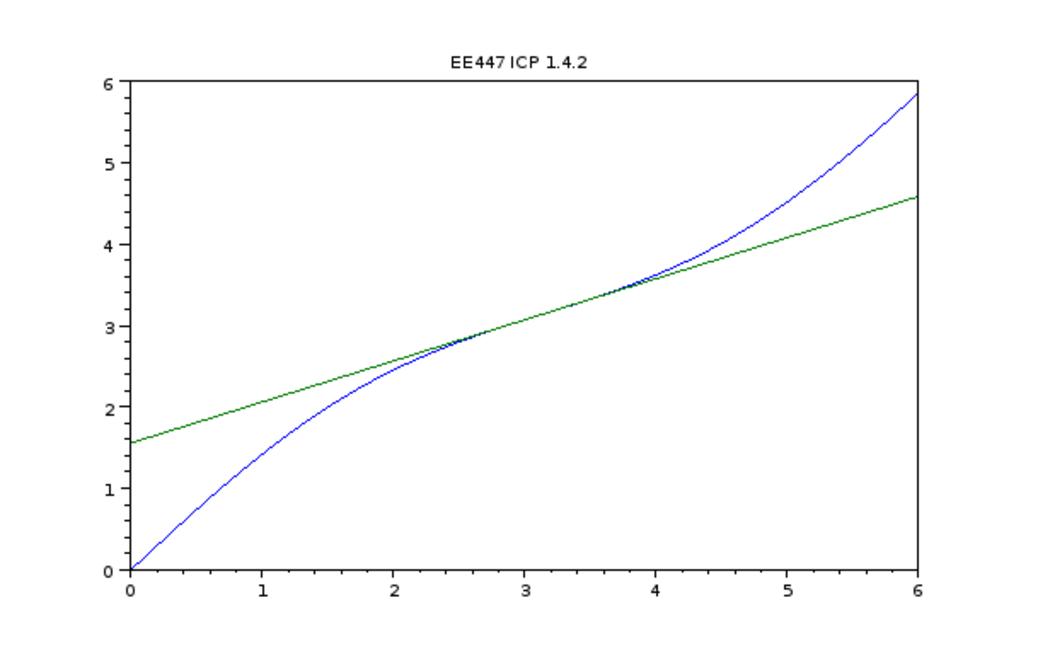
\includegraphics[width=3.5in]{icp142_plota.png}

\end{solution}
	%<*>


%%%%** Section 1.5
\subsection{Linearization}

 Linearize
\[
A_2 \ddot{x} + A_1(\dot{x}+0.2\dot{x}^3) + A_0x  = f(t)
\]
about the point $\dot{x} = 0$, so that it forms a LODE.
{\bf Hint: }  The function is actually non linear in $\dot{x}$ so the thing we need to linearize is actually

\[
A_2 \ddot{x} + A_1(\dot{x}+0.2\dot{x}^3) + A_0x  = f(\dot{x})
\]

	%<*n>
\begin{solution}
\[
f(\dot{x}) |_{\dot{x} = 0}  = A_2\ddot{x} + A_0x
\]
\[
\frac{d}{d\dot{x}}|_{\dot{x}=0} = A_1 + 0.6A_1\dot{x}^2  |_{\dot{x} = 0} = A_1
\]
\[
\hat{f}(\dot{x}) = A_2 \ddot{x} + A_0 x + A_1\dot{x}
\]
writing this in the more traditional LODE order:
\[
\hat{f}(\dot{x}) = A_2 \ddot{x}+ A_1\dot{x} + A_0 x
\]

Note that because we are linearizing around $x=0$ {\it and} because our nonlinearity is a polynomial,   $\hat{f}(x)$ is just $f(x)$ with the nonlinaer term dropped.

\end{solution}

	%<*>
%%%%** Section 1.5.1 
\subsubsection{} \label{LinearizePtwo} A spring is measured at several applied forces and the resulting data fits the function
\[
f(x) =0.02x^4  +  0.65x^2+ 16x
\]
Linearize this function about the point $x=0$.

	%<*n>
\begin{solution}
As we have seen before if the function, $f(x)$ is
\begin{enumerate}
  \item a polynomial
  \item being linearized about $x=0$
\end{enumerate}

Then we can linearize simply by taking the linear term:

\[
\hat{f}(x) = 16x
\]
\end{solution}



	%<*>
%%%%** Section 1.5.2 
\subsubsection{}
Using the result of \ref{LinearizePtwo}, for what range of $x$ is the error between $f(x)$ and the linearized function $\hat{f}(x)$ less than 10\%?
{\bf Hint:} find the result numerically.


	%<*n>
\begin{solution}
The error is
\[
e(x) = f(x) - \hat{f}(x)
\]
\[
e(x) = 0.02x^4  +  0.65x^2+ 16x - 16x  = 0.02x^4  +  0.65x^2
\]
(divide by $f(x)$ to get percent)

Using the calculator or computer:

\begin{center}
\begin{tabular}{cr}
$x$      &   $e(x)/f(x)$ \\ \hline
-2.5	& 13\% \\
-2	& 10\% \\
-1.5	& 7\% \\
-1	& 4.3\% \\
1	& 4.0\% \\
1.5	& 6.1\% \\
2.0	& 8.4\% \\
2.5	& 10.8\% \\
\end{tabular}
\end{center}

Thus, the error is less than $10\%$ for roughly
\[
-2.0 \leq x \leq 2.3
\]
\end{solution}






%%%%%%%%%%%%%%%%%%%%%%%%%%%%%%%%%%%%%%%%%%%%%%%%%%%%%%%%%%%%%%%%%%%%%%%%%%%%%%%%%%%%%%%%%%%%%%%
	%<*>
\newpage
%%%%** Section 2 
\section{Translational Dynamical Systems}

	%<*>
%%%%** Section 2.1
\subsection{}

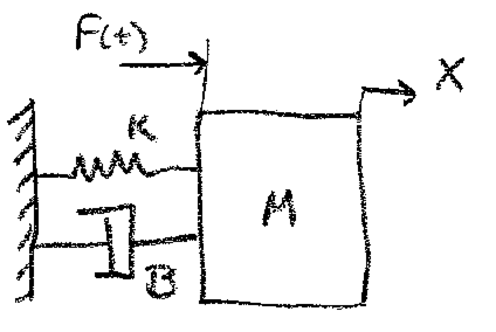
\includegraphics[width=42mm]{00449a.png}

%%%%** Section 2.1.1 
\subsubsection{} Find the equation of motion (EOM) in ODE form for $x(t)$.

	%<*n>
\begin{solution}
Eqn of motion is sum of forces on the mass:
\[
M\ddot{x} + B\dot{x} + Kx = F(t)
\]
\end{solution}

	%<*>
%%%%** Section 2.1.2 
\subsubsection{} Find $\frac{X(s)}{F(s)}$

	%<*n>
\begin{solution}
Laplace Transform:
\[
MX(s)s^2+BX(s)s+KX(s) = F(s)
\]
Factor
\[
X(s)\left( Ms^2+Bs+K \right ) = F(s)
\]
\[
\frac{X(s)}{F(s)} = \frac {1}  { Ms^2+Bs+K }
\]
Normalize

\[
\frac{X(s)}{F(s)} = \frac {1/M}  { s^2+\frac{B}{M}s+\frac{K}{M} }
\]

\end{solution}


	%<*>
%%%%** Section 2.2
\subsection{}
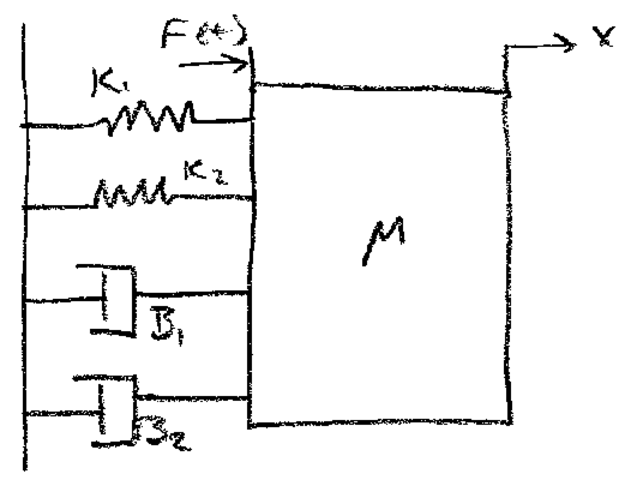
\includegraphics[width=54mm]{00450a.png}

%%%%** Section 2.2.1 
\subsubsection{} Find the differential equation.

	%<*n>
\begin{solution}
Eqn of motion is sum of forces on the mass:
\[
M\ddot{x} + B_1\dot{x} + B_2\dot{x} + K_1x + K_2x = F(t)
\]
\end{solution}

	%<*>
%%%%** Section 2.2.2 
\subsubsection{}  Find the transfer function $\frac{X(s)}{F(s)}$

	%<*n>
\begin{solution}
Taking LT and factoring:
\[
X(s) \left ( Ms^2 + (B_1+B_2)s+(K_1+K_2) \right ) = F(s)
\]

Normalize

\[
\frac{X(s)}{F(s)} = \frac {1/M}  { s^2+\frac{B_1+B_2}{M}s+\frac{K_1+K_2}{M} }
\]

\end{solution}




	%<*>
%%%%** Section 2.3
\subsection{}\label{2masstranslation}

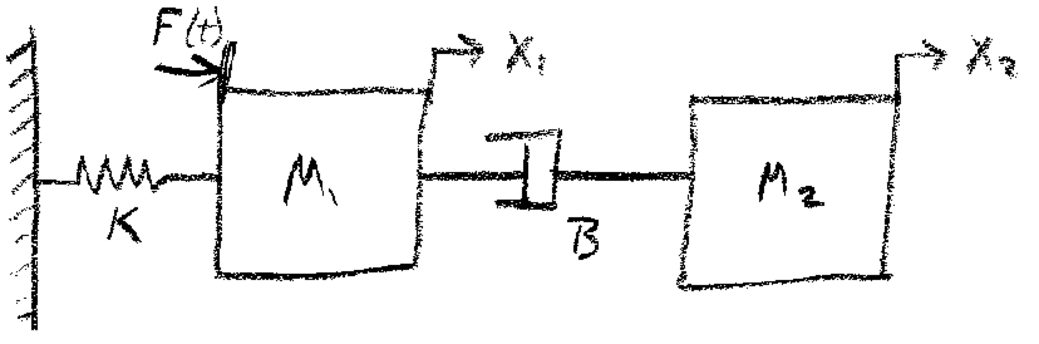
\includegraphics[width=88mm]{00451a.png}

%%%%** Section 2.3.1 
\subsubsection{} Find the equation of motion (EOM) in ODE form for $M_1$ and $M_2$.

	%<*n>
\begin{solution}
EOMS:

\[
M_1\ddot{x}_1 + Kx_1+ B(\dot{x}_1-\dot{x}_2) = F(t)
\]
\[
M_2\ddot{x}_2 +  B(\dot{x}_2-\dot{x}_1) = 0
\]

\end{solution}
	%<*>

%%%%** Section 2.3.2 
\subsubsection{} Find $\frac{X_2(s)}{F(s)}$

	%<*n>
\begin{solution}

\[
\frac{X_2(s)}{F(z)} = \frac  {B/(M_1M_2)}     {s^3 + \frac{B(M_1+M_2)}{M_1M_2}s^2 + \frac{K}{M_1}s + \frac{BK}{M_1M_2}}
\]

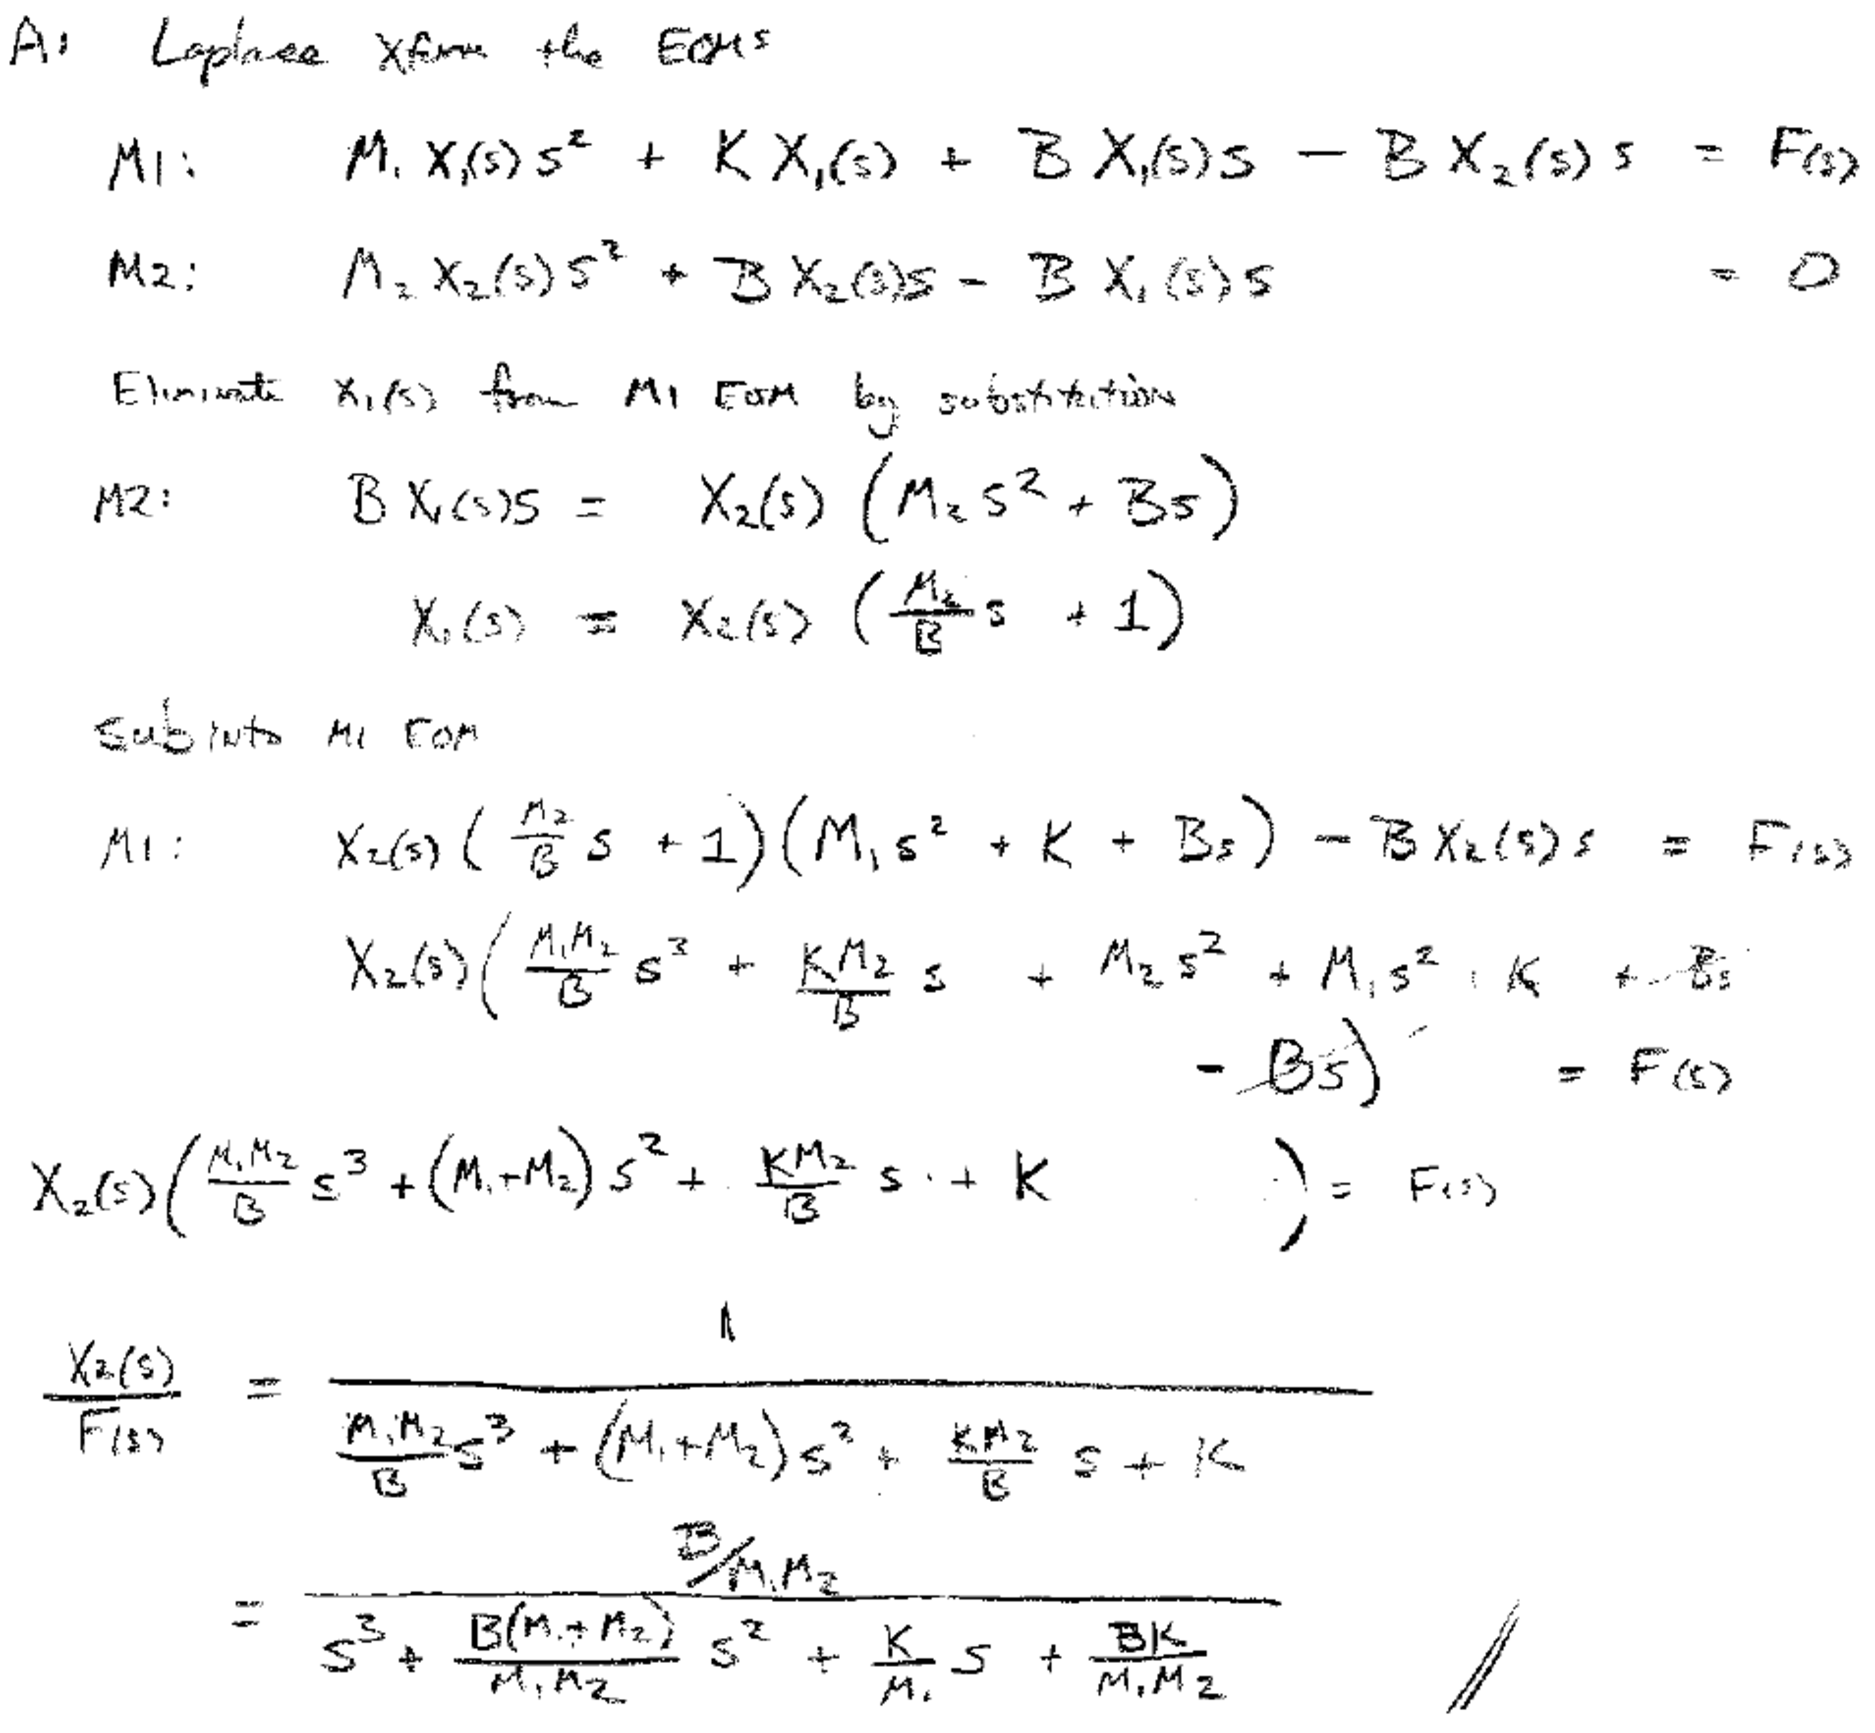
\includegraphics[width=6.25in]{00942a.png}
\end{solution}
	%<*>


%%%%** Section 2.4
\subsection{}


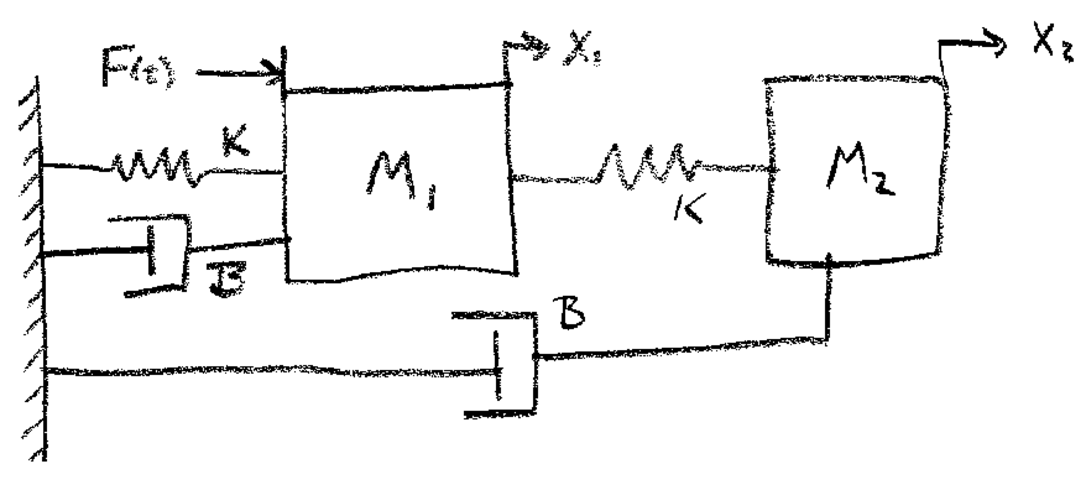
\includegraphics[width=92mm]{00452a.png}

Find the equations of motion (EOMs)  and the transfer function  $\frac{X_1(s)}{F(s)}$


	%<*n>
\begin{solution}
EOMS:
\[
M_1\ddot{x}_1+Kx_1+B\dot{x}_1+K(x_1-x_2) = F(t)
\]
\[
M_2\ddot{x}_2+B\dot{x}_2+K(x_2-x_1) = 0
\]
LT:
\[
X_1(s)\left( M_1s^2+B_s+2K) + X_2(s)(-K)  \right ) = F(s)
\]
\[
X_2(s)\left( M_2s^2+B_s+K) + X_1(s)(-K)  \right ) = 0
\]
Transfer Function:

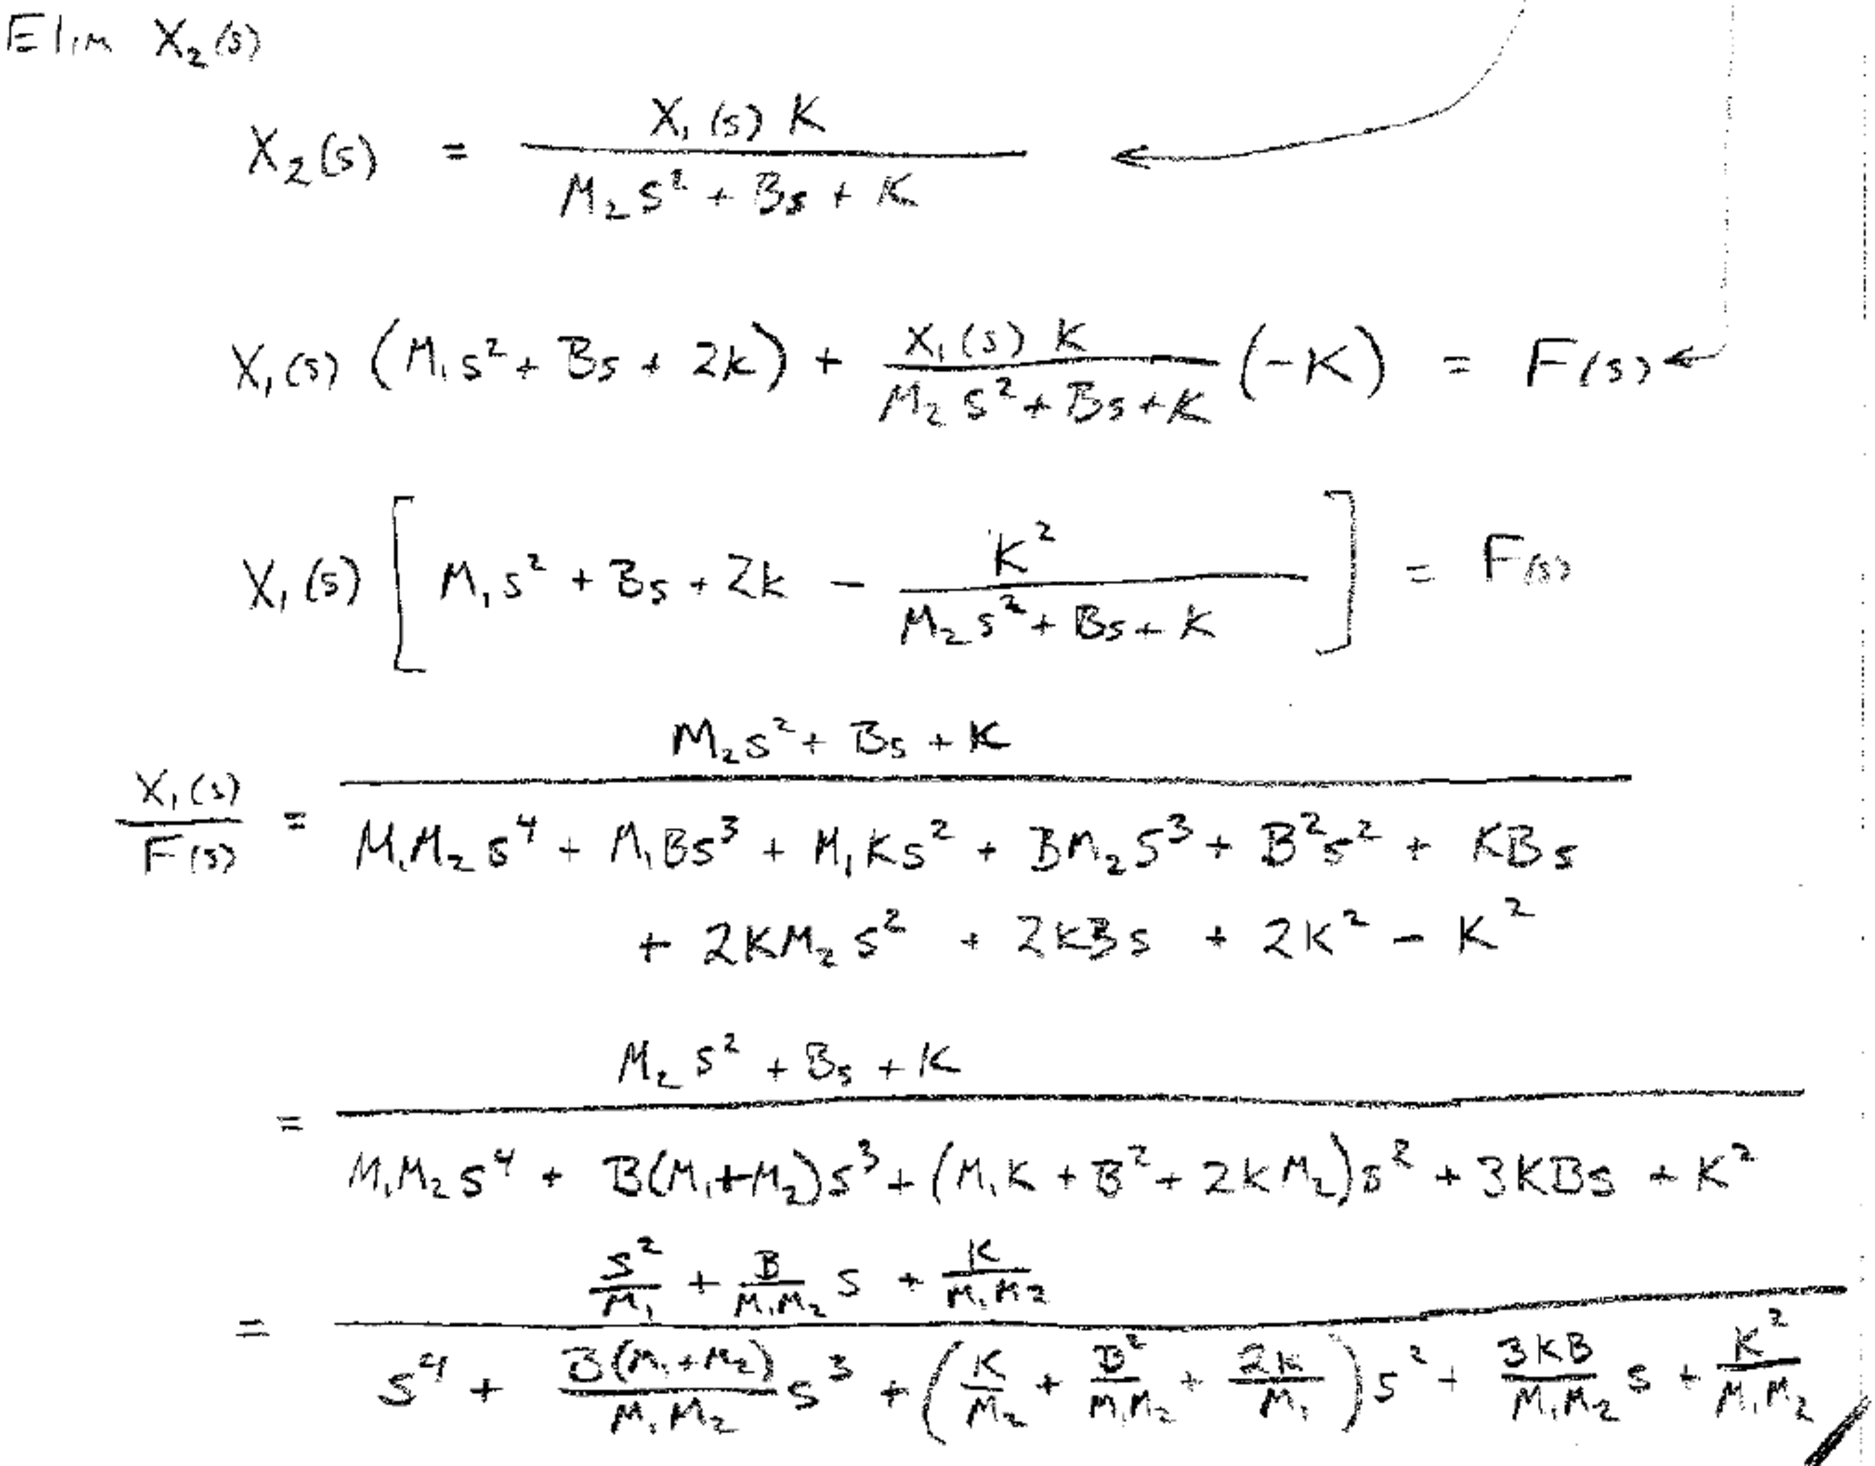
\includegraphics[width=6.25in]{00943a.png}

\end{solution}
	%<*>


	%<*>
%%%%** Section 2.5
\subsection{}
 A system has the transfer function
\[
G(s) =  \frac{X(s)}{F(s)} = \frac{1}{M_1s^2+(B_1+B_2)S + K/M_1}
\]

%%%%** Section 2.5.1 
\subsubsection{}
Normalize the transfer function $G(s)$.

	%<*n>
\begin{solution}
\[
\frac{X(s)}{F(s)} = \frac{1/M_1} {s^2+\frac{B_1+B_2}{M_1}s + K/M_1}
\]
\end{solution}

%%%%** Section 2.5.2 
\subsubsection{}
 Analyzing $G(s)$ for the values $B_1=5$, $B_2 = 7$, $M_1 = 10$, $K=200$,
 find the characteristic polynomial and the poles.


	%<*n>
\begin{solution}
\[
\frac {X(s)}  {F(s)} = \frac { 0.1 }  { s^2 + 1.2s + 20}
\]
Poles:
\[
p = \frac {-1.2\pm\sqrt{1.2^2 - 4\times20}}   {2} = -0.6 \pm j 4.43
\]
\end{solution}
	%<*>

%%%%** Section 2.6
\subsection{} For the following transfer function, plot the poles and zero(s) in the complex plane.

\[
H(s) = \frac   {s+20}  {s^2 + 25s + 256.25}
\]

	%<*n>
\begin{solution}

Zeros:  $s=-20$

Poles: $s = -12.5\pm10j$

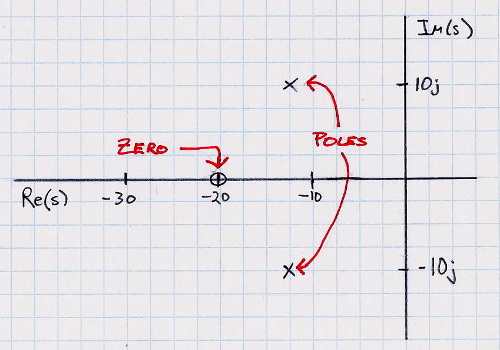
\includegraphics[width=110mm]{01076.png}

\end{solution}
	%<*>


%\end{frame}  %%%%%%%%%%%%%%%%%%%%%%%%%%%%%%%%%%%%%%%%%%%%%%%%%%%%%%%%%%%%




%%%%%%%%%%%%%%%%%%%%%%%%%%%%%%%%%%%%%%%%%%%%%%%%%%%%%%%%%%%%%%%%%%%%%%%%%%%%%%%%%%%%%%%%%%%%%%%
	%<*>
\newpage
%%%%** Section 3 
\section{Rotational Dynamical Systems and State Space}

	%<*>
%%%%** Section 3.1
\subsection{}

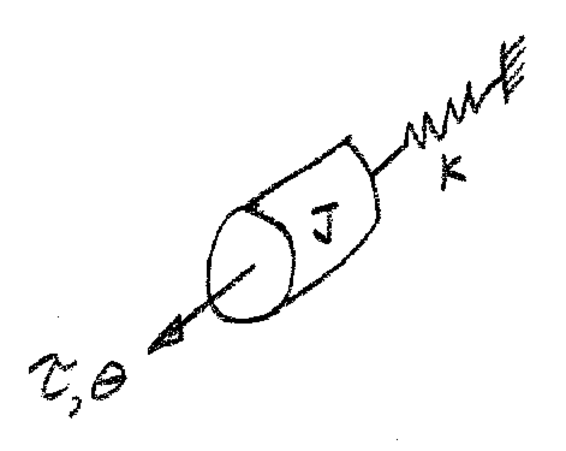
\includegraphics[width=48mm]{00460a.png}

a) Find the equation of motion (EOM)

	%<*n>
\begin{solution}
EOM:
\[
J\ddot{\theta} + K\theta = \tau
\]
\end{solution}
	%<*>

b) Find $\frac{\theta(s)}{\tau(s)}$\label{simplerotary}

	%<*n>
\begin{solution}
\[
\theta(s) \left ( Js^2+K \right ) = \tau(s)
\]
\[
\frac{\theta(s)} {\tau(s)}   =  \frac {1/J}    {s^2 + K/J}
\]
\end{solution}
	%<*>


	%<*>
%%%%** Section 3.2
\subsection{}

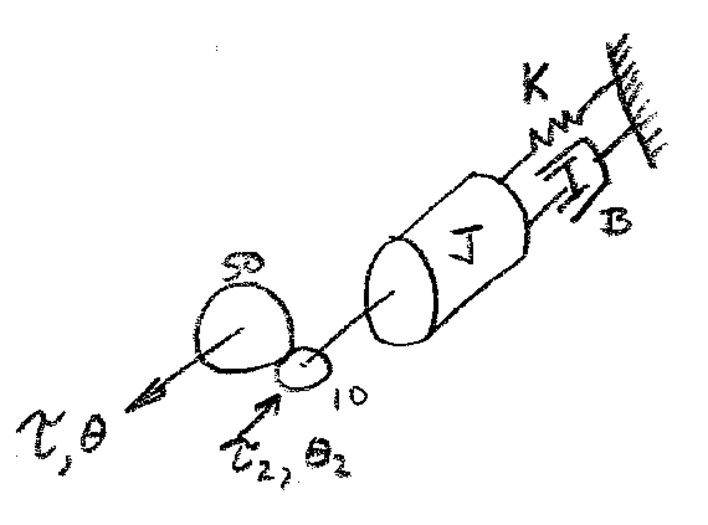
\includegraphics[width=60mm]{00461a.png}

Write the EOM and get $\frac{\theta(s)}{\tau(s)}$.

	%<*n>
\begin{solution}
\[
\tau_2 = \frac{10}{50}\tau \qquad \theta_2 = \frac{50}{10}\theta
\]
Using \ref{simplerotary}b but adding in a damper:
\[
\frac{\theta_2(s)} {\tau_2(s)}   =  \frac {1/J}    {s^2 + B/Js+ K/J}
\]
Substituting:
\[
\frac{\theta(s)} {\tau(s)}   =
\frac{10/50\theta_2(s)} {50/10\tau_2(s)}   = \frac{1}{25} \frac{\theta_2(s)} {\tau_2(s)}  =  \frac {1/(25J)}    {s^2  + (B/J)s+ K/J}
\]

\vspace{0.2in}
{\bf Alternate Method:}

Use the "$n^2$" rule to scale J, B, K and eliminate the gears:
\[
n^2 = 25, \quad \hat{J} = 25J, \quad \hat{B} = 25B, \quad \hat{K} = 25K
\]
\[
\frac{\theta(s)} {\tau(s)}   =
  \frac {1/\hat{J}}    {s^2 + (\hat{B}/\hat{J})s+ \hat{K}/\hat{J}}
\]
Expanding the "hats" and canceling gives:

\[
\frac{\theta(s)} {\tau(s)}   =
\frac {1/25{J}}    {s^2 + (25{B}/25{J})s+ 25{K}/25{J}} =  \frac {1/(25J)}    {s^2  +(B/J)s+ K/J}
\]
\end{solution}
	%<*>


%\end{frame}  %%%%%%%%%%%%%%%%%%%%%%%%%%%%%%%%%%%%%%%%%%%%%%%%%%%%%%%%%%%%


	%<*>
%%%%** Section 3.3
\subsection{}\label{2mass10to60}

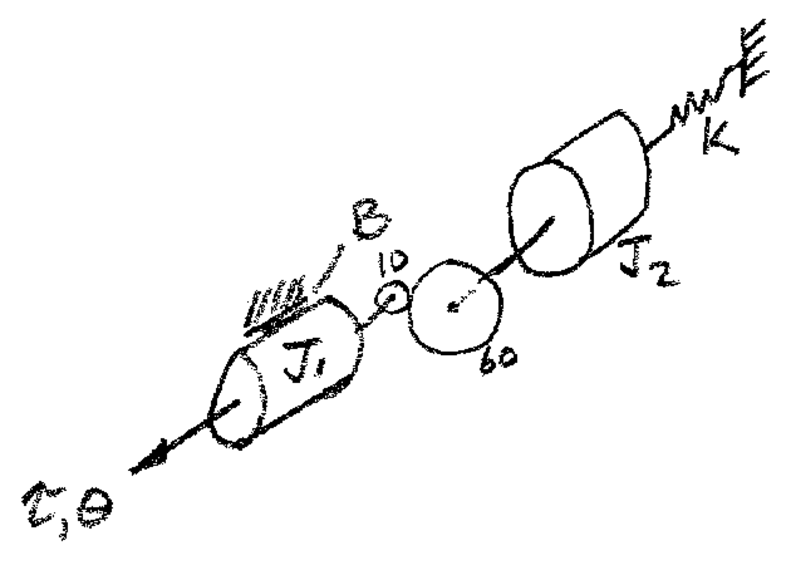
\includegraphics[width=67mm]{00462a.png}

Find the equation of motion (EOM) and the transfer function $\frac{\theta(s)}{\tau(s)}$


	%<*n>
\begin{solution}
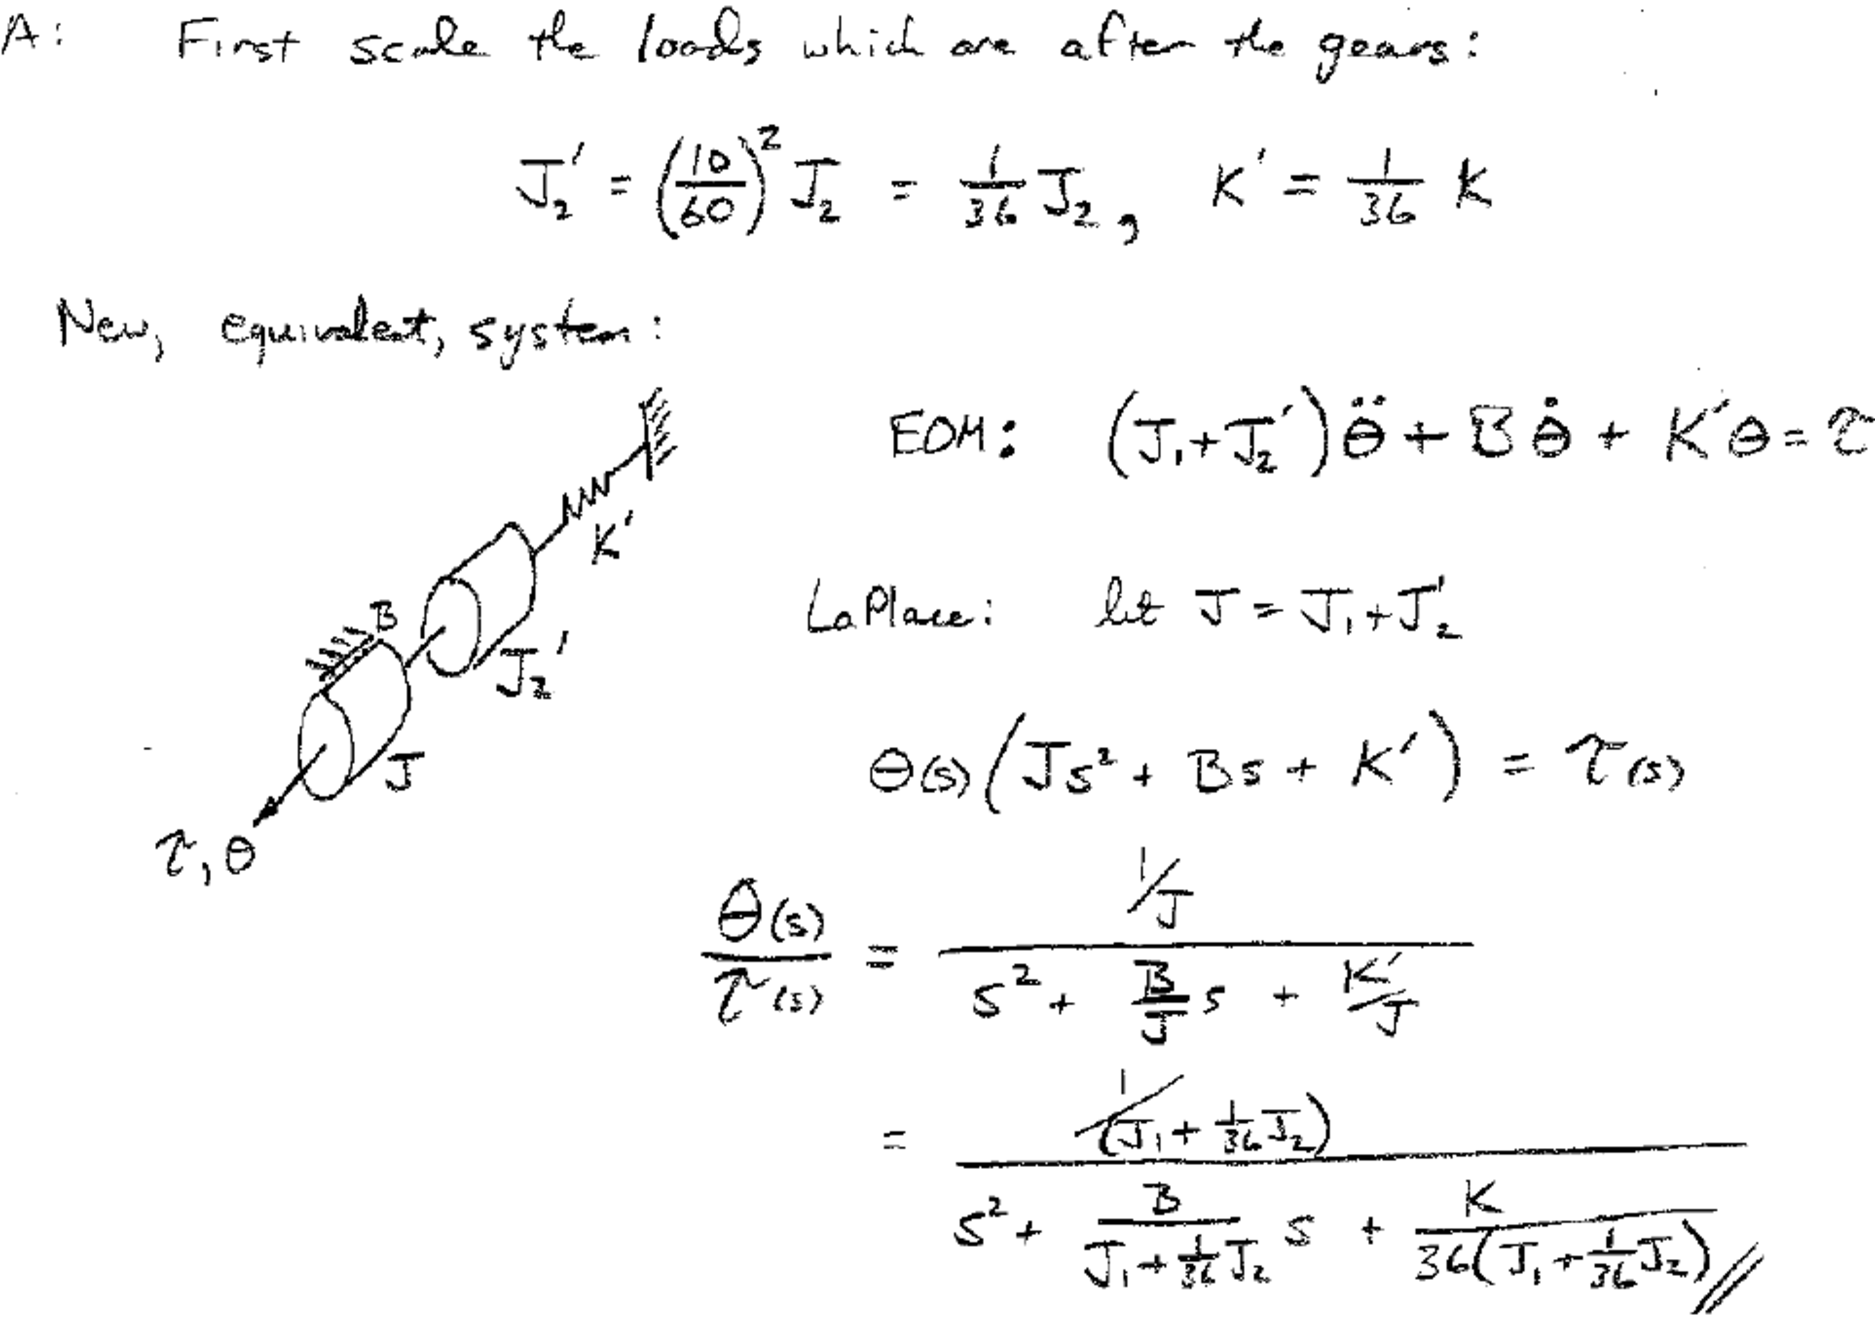
\includegraphics[width=6.25in]{00945a.png}
\end{solution}
	%<*>

%\end{frame}  %%%%%%%%%%%%%%%%%%%%%%%%%%%%%%%%%%%%%%%%%%%%%%%%%%%%%%%%%%%%


	%<*>
%%%%** Section 3.4
\subsection{}
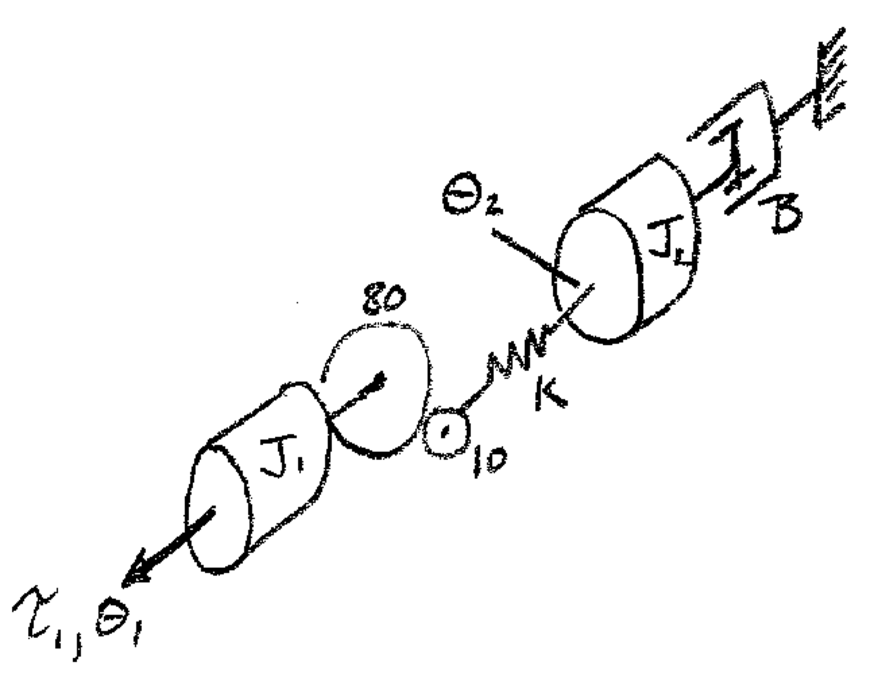
\includegraphics[width=74mm]{00463a.png}

Find the equations of motion (EOMs)  and the transfer function  $\frac{\theta_1(s)}{\tau_1(s)}$


	%<*n>
\begin{solution}
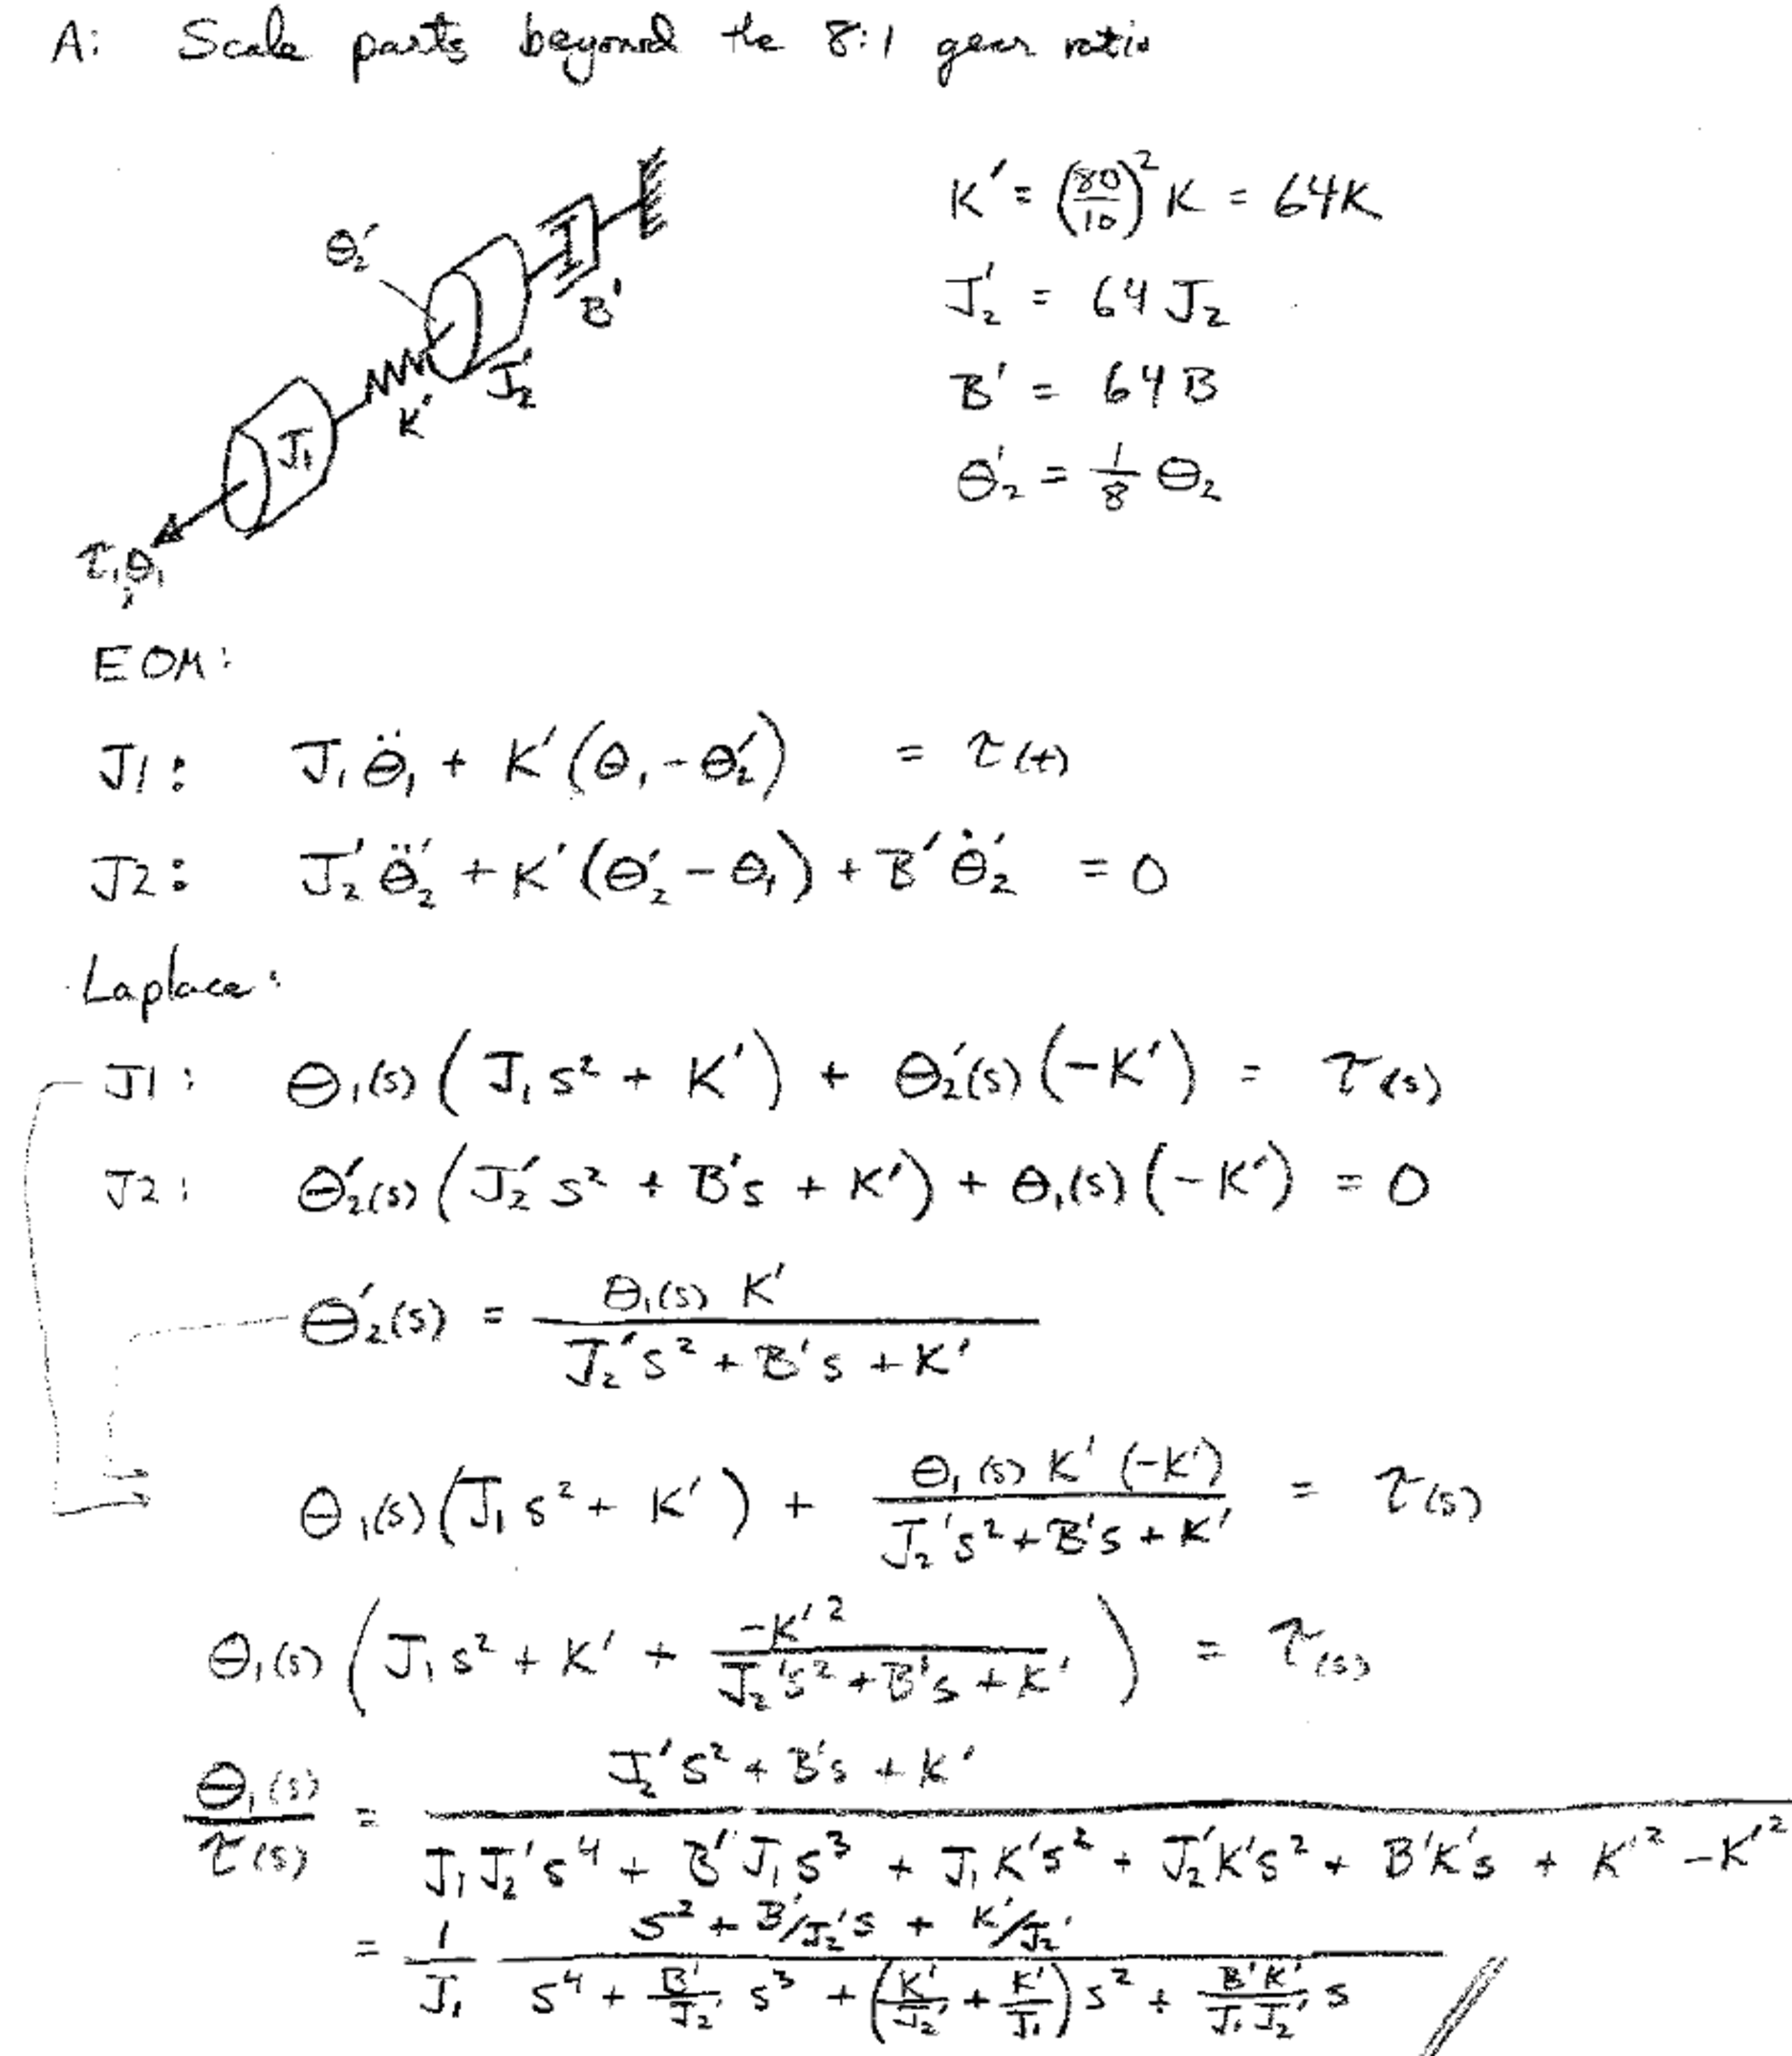
\includegraphics[width=6.25in]{00946a.png}
\end{solution}
	%<*>

%\end{frame}  %%%%%%%%%%%%%%%%%%%%%%%%%%%%%%%%%%%%%%%%%%%%%%%%%%%%%%%%%%%%


	%<*>
%%%%** Section 3.5
\subsection{}

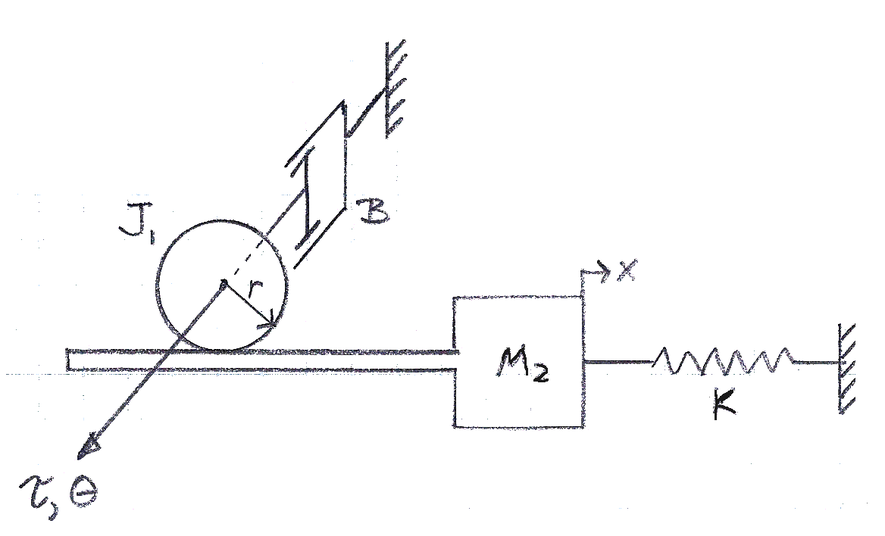
\includegraphics[width=75mm]{00960aa.png}

Find the equations of motion (EOMs)  and the transfer function  $\frac{\theta(s)}{\tau(s)}$. (Note, unlike many problems, we will consider the inertia of the gear ($J_1$) in this problem.)

	%<*n>
\begin{solution}
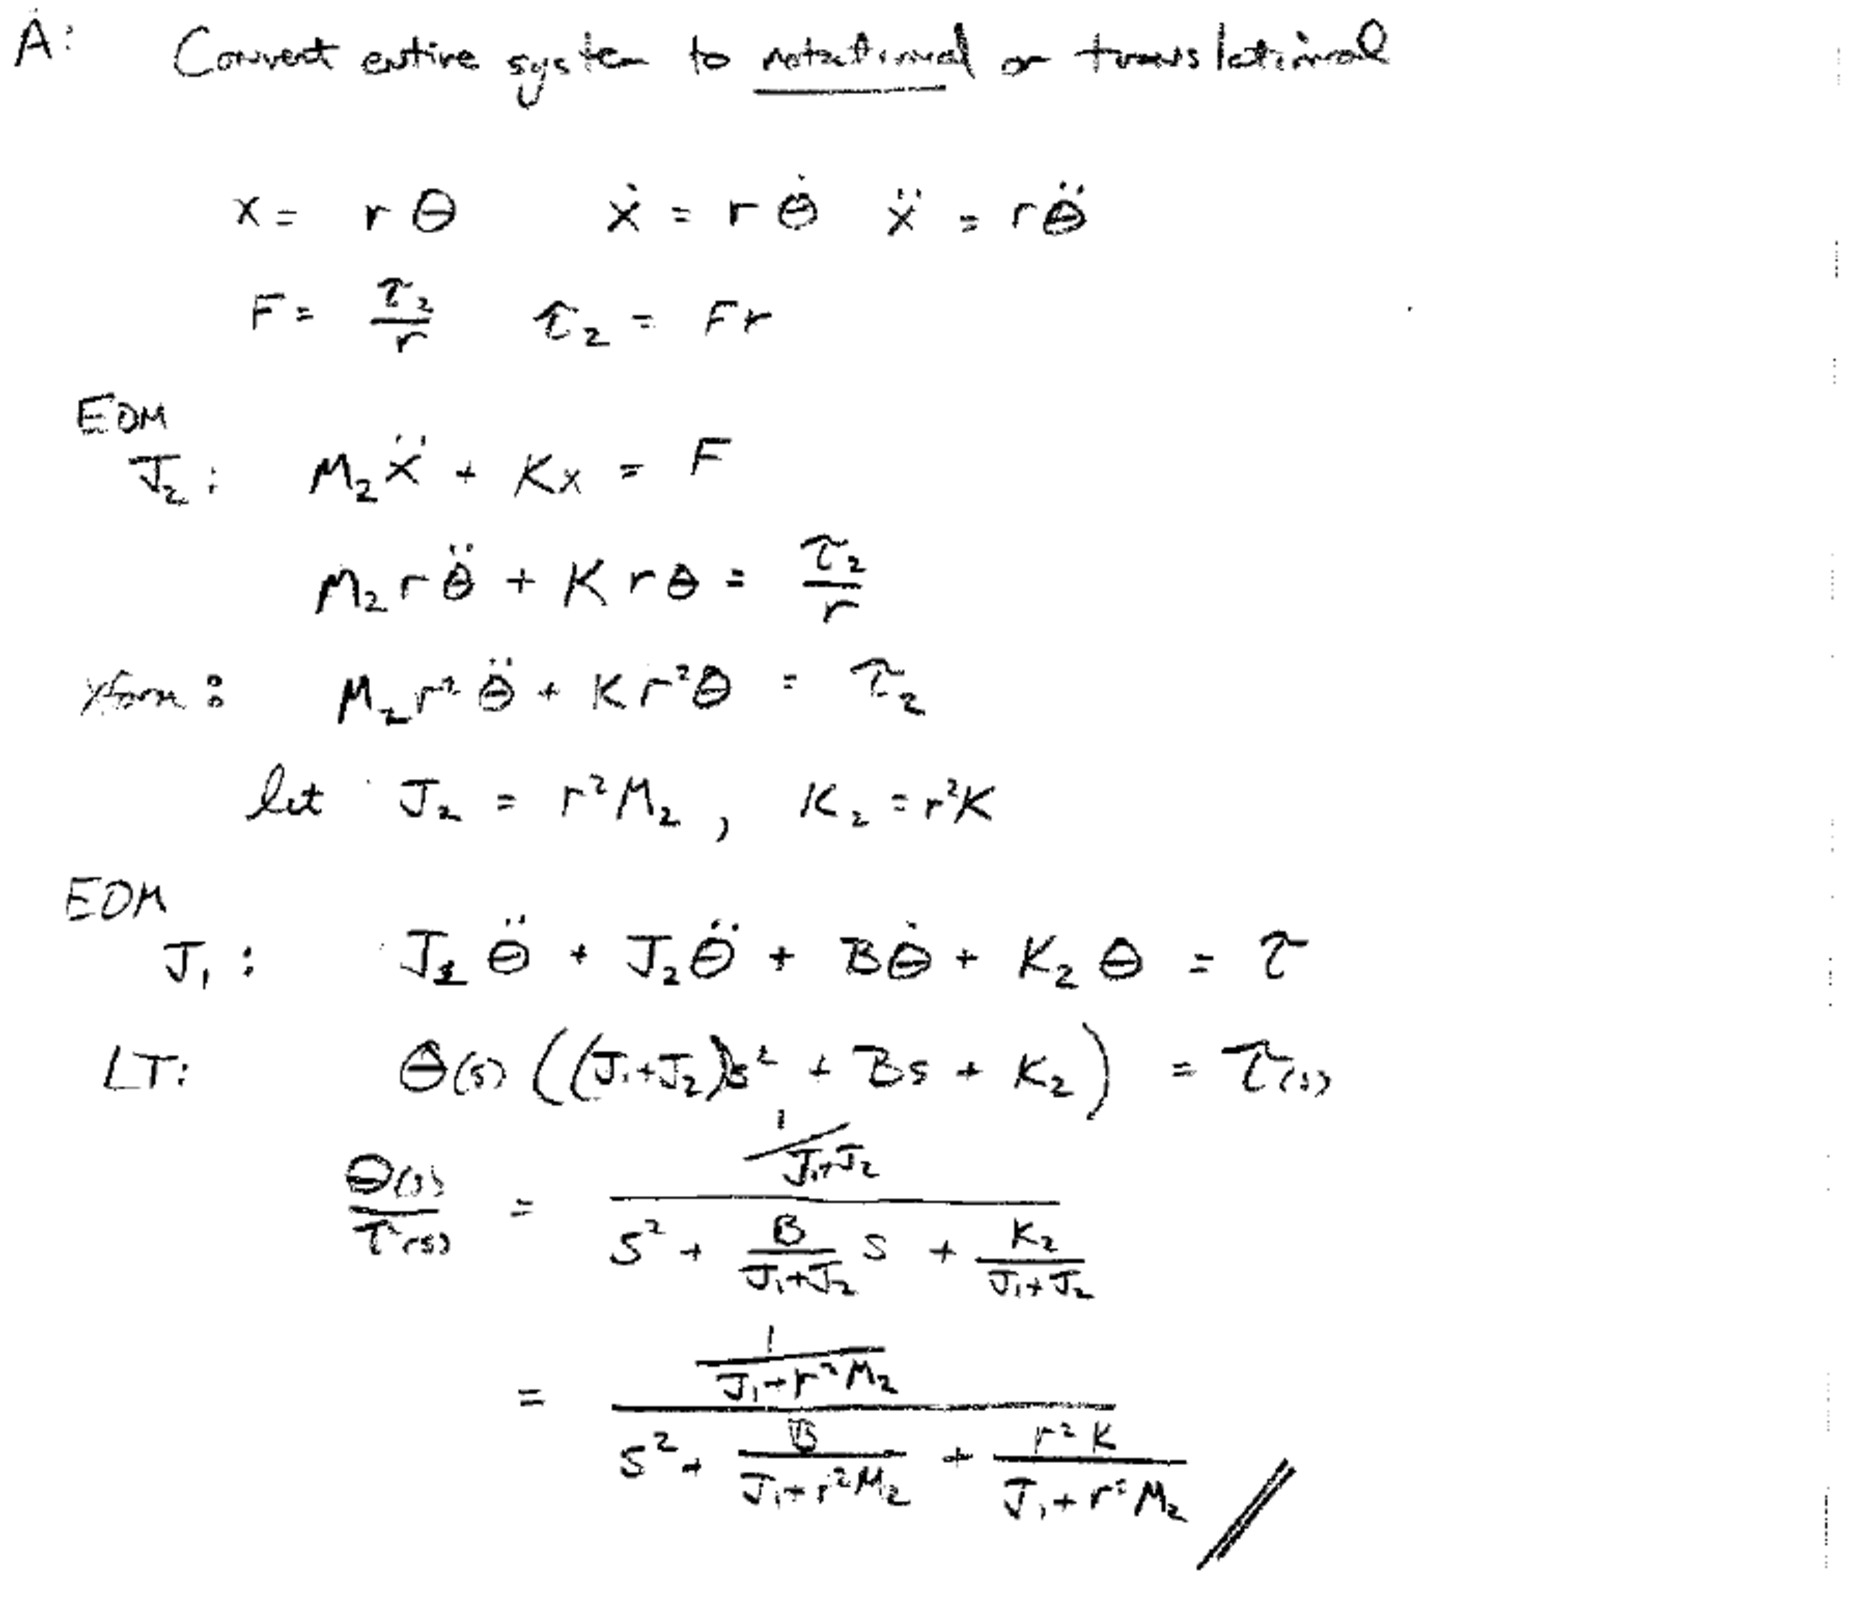
\includegraphics[width=6.25in]{00947a.png}
\end{solution}
	%<*>


%\end{frame}  %%%%%%%%%%%%%%%%%%%%%%%%%%%%%%%%%%%%%%%%%%%%%%%%%%%%%%%%%%%%


%%%%%%%%%%%%%%%%%%%%%%%%%%%%%%%%%%%%%%%%%%%%%%%%%%%%%%%%   State Space

\section*{State Space}

%%%%** Section 3.6
\subsection{}\label{ICPss_1mass}
%%%%** Section 3.6.1 
\subsubsection{}
Represent the system of Problem \ref{2mass10to60} in state space. Do not worry about the second
equation (the ``output equation", $Y = CX+DU$).


	%<*n>
\begin{solution}
Rearranging the EOM and noting that $n^2 = 36$,
\[
\ddot{\theta} = -\frac{B}{(J_1+J_2/36)}\dot{\theta} - \frac{K}{(36J_1+J_2)}\theta + \frac{\tau}{(J_1+J_2/36)}
\]
Let
\[
X = \begin{bmatrix} \theta \\ \dot{\theta} \end{bmatrix}
\qquad
\dot{X} = \begin{bmatrix} \dot{\theta}\\ \ddot{\theta} \end{bmatrix}
\]
then converting to a matrix equation:
\[
\dot{X}  = AX  + BU
\]
\[
\dot{X} = \begin{bmatrix}0&1\\
\frac{-K}{(36J_1+J_2)} & \frac{-B}{(J_1+J_2/36)} \end{bmatrix} X +
\begin{bmatrix}0 \\ \frac{1}{(J_1+J_2/36)}\end{bmatrix} \tau
\]
\end{solution}
	%<*>


%%%%** Section 3.6.2 
\subsubsection{}
For
\[
J_1 = 10 \quad J_2 = 100 \quad K=20 \quad B=5
\]
Find $A$,$B$, in numerical form

	%<*n>
\begin{solution}
Plugging in to previous result:
\[
A = \begin{bmatrix} 0 & 1 \\ -43.5\times10^{-3} & -391\times10^{-3}
\end{bmatrix}
\qquad
B = \begin{bmatrix} 0 \\ -78.3\times10^{-3} \end{bmatrix}
\]
\end{solution}
	%<*>


%%%%** Section 3.7
\subsection{}\label{ICPss_2mass}
Find the State Space representation for the translational system of Problem \ref{2masstranslation}
(also ignore the output equation).

Hint: the EOMs of that problem were:

\begin{align*}
&M_1\ddot{x}_1+Kx_1+B(\dot{x}_1-\dot{x}_2) = F(t)  \\
&M_2\ddot{x}_2+B(\dot{x}_2-\dot{x}_1) = 0
\end{align*}
The state variables are all the motion variables from which we can get a kinetic (mass) or potential
(spring) energy:  $x_1, \dot{x}_1,x_2, \dot{x}_2$.


	%<*n>
\begin{solution}
Rewriting the EOMs:

\begin{align*}
\ddot{x}_1 &= -\frac{B}{M_1}\dot{x}_1 +\frac{B}{M_1}\dot{x}_2 -\frac{K}{M_1}{x}_1 + \frac{1}{M_1}f(t)  \\
\ddot{x}_2 &= -\frac{B}{M_2}\dot{x}_2 +\frac{B}{M_2}\dot{x}_1
\end{align*}
Let
\[
X       = \begin{bmatrix}x_1\\\dot{x}_1\\x_2\\\dot{x}_2\end{bmatrix} \qquad
\dot{X} = \begin{bmatrix}\dot{x}_1\\\ddot{x}_1\\\dot{x}_2\\\ddot{x}_2\end{bmatrix} \qquad
\]
Then plugging in:
\[
A = \begin{bmatrix}0&1&0&0\\
-\frac{K}{M_1} &-\frac{B}{M_1} & 0  &\frac{B}{M_1} \\
0&0&0&1\\
0 &\frac{B}{M_2} & 0 &-\frac{B}{M_2}
\end{bmatrix}
\qquad  B =
\begin{bmatrix}0 \\ \frac{1}{M_1}\\ 0 \\ 0\end{bmatrix}
\]

\end{solution}
	%<*>


%%%%** Section 3.8
\subsection{}
Find the output equation matrices $C$ and $D$ for the two previous ICPs.  Assume the output variable
for the first problem is $\theta$ and for the second problem there is a two-vector output:
\[
Y = \begin{bmatrix}x_1\\\dot{x}_1\end{bmatrix}
\]

	%<*n>
\begin{solution}
Problem \ref{ICPss_1mass}:
\[
Y = \theta = \begin{bmatrix}1&0\end{bmatrix}X + 0 U
\]
so
\[
C = \begin{bmatrix}1&0\end{bmatrix}  \qquad D = 0
\]

\noindent
Problem \ref{ICPss_2mass}

\[
Y = \begin{bmatrix}x_1\\\dot{x}_1\end{bmatrix} = \begin{bmatrix}1&0&0&0 \\ 0&1&0&0\end{bmatrix}X + 0 U
\]
so
\[
C = \begin{bmatrix}1&1&0&0 \\ 0&1&0&0\end{bmatrix}  \qquad D = 0
\]
\end{solution}
Note that $X$ vector is different between problems  \ref{ICPss_1mass} and \ref{ICPss_2mass}.
	%<*>




%%%%%%%%%%%%%%%%%%%%%%%%%%%%%%%%%%%%%%%%%%%%%%%%%%%%%%%%%%%%%%%%%%%%%%%%%%%%%%%%%%%%%%%%%%%%%%%
	%<*>
\newpage
%%%%** Section 4 
\section{\EEcourse In Class Problems: Plotting Frequency Response}
%%%%** Section 4.1
\subsection{Decibels}


%
%Express the following in dB:
%\begin{enumerate}
%	\item 1000 = \_\_\_\_\_\_ dB
%	\item $\sqrt{10}\times10^5 = $ \_\_\_\_\_\_ dB
%	\item 0.01   = \_\_\_\_\_\_ dB
%	\item 0.5 = \_\_\_\_\_\_ dB
%	\item $\frac{1}{\sqrt{2}}$ = \_\_\_\_\_\_ dB
%\end{enumerate}
%
	%<*n>
\begin{solution}
Express the following in dB:
\begin{enumerate}
	\item 1000 = \_\_60\_\_ dB
	\item $\sqrt{10}\times10^5 = 20 \left ( \log(10)/2 \right) + 20\times 5 = $ \_\_110\_\_ dB
	\item $0.01 =20\log(10^{-2}) = 20\times(-2) = $\_\_-40\_\_ dB
	\item 0.5 = \_\_-6\_\_ dB
	\item $\frac{1}{\sqrt{2}} = \frac{-6dB}{2}$ = \_\_-3\_\_ dB
\end{enumerate}

\end{solution}
	%<*>

%\end{frame}  %%%%%%%%%%%%%%%%%%%%%%%%%%%%%%%%%%%%%%%%%%%%%%%%%%%%%%%%%%%%



	%<*>
%%%%** Section 4.2
\subsection{}
Plot the poles of the following 2nd order transfer function:
\[
G(s) = \frac{10}{s^2 + 6.32\zeta s + 10}
\]
for $\zeta = \{ 1, 0.5, 0.1 \}$

	%<*n>
\begin{solution}
\[
\zeta = 1.0 \qquad CP = s^2+6.32s+10 \qquad \omega_n = \sqrt{10} = 3.16
\]
\[
p = -3.16\pm 0.12j
\]
\[
\zeta = 0.5 \qquad CP = s^2+3.16s+10 \qquad \omega_n = \mathrm{same}  = 3.16
\]
\[
p = -1.58\pm 2.7j
\]
\[
\zeta = 0.1 \qquad CP = s^2+0.632s+10 \qquad \omega_n = \mathrm{same}  = 3.16
\]
\[
p = -0.316\pm 3.15j
\]

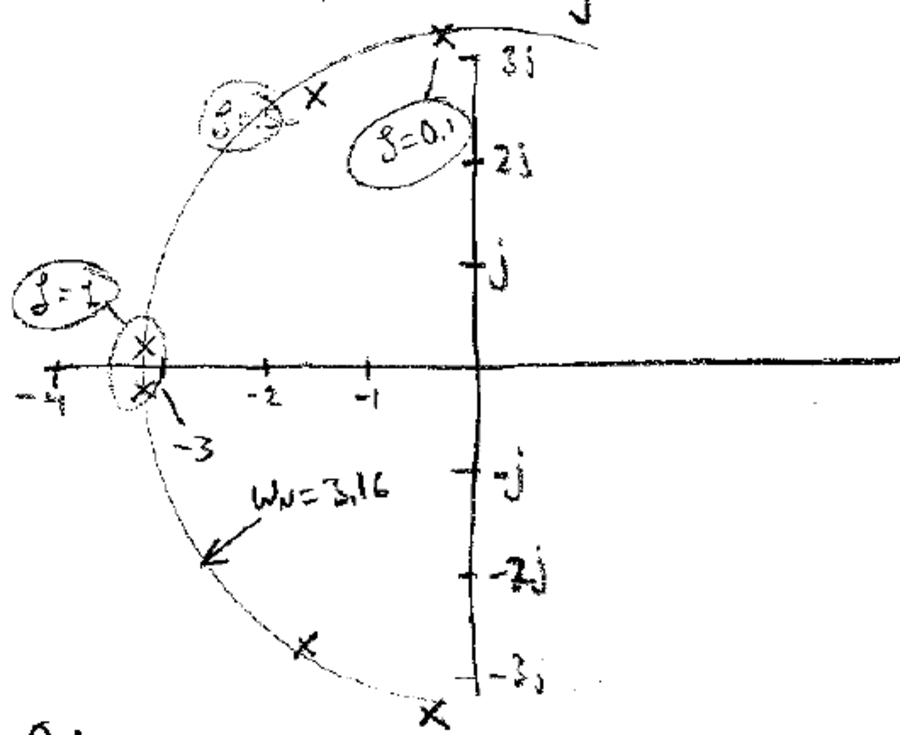
\includegraphics[width=3.0in]{00948a.png}

\end{solution}
	%<*>

%\end{frame}  %%%%%%%%%%%%%%%%%%%%%%%%%%%%%%%%%%%%%%%%%%%%%%%%%%%%%%%%%%%%


	%<*>
%%%%** Section 4.3
\subsection{}
Let
\[
G(s) = \frac{1000}{s+1000}
\]

Draw $|G(j\omega)|$ and $\angle G(j\omega)$.

	%<*n>
\begin{solution}

Note: this solution illustrates a rather slow method to achieve full understanding of the fully valid, but much faster procedure of drawing asymptotes directly.

\paragraph{Magnitude:} substitute $s=j\omega$ (sinusoidal steady-state response at frequency $\omega$)

Approximate for three frequency ranges to get asymptotes (slow beginner method)
\[
\omega<<1000 \qquad |G(j\omega)| \approx |\frac{1000}{1000} = 1 = 0dB
\]
\[
\omega>>1000 \qquad |G(j\omega)| \approx |\frac{1000}{j\omega}| = 1000 \omega^{-1} = 60db - 20\log(\omega) db \quad (-20dB/\mathrm(dec))
\]
\[
\omega=1000 \qquad |G(j\omega)|    =     |\frac{1000}{1000+j1000}| = |\frac{1}{1+j}| = \frac{1}{\sqrt{2}} = 0.707 = -3dB
\]

Plotting asymptotes:

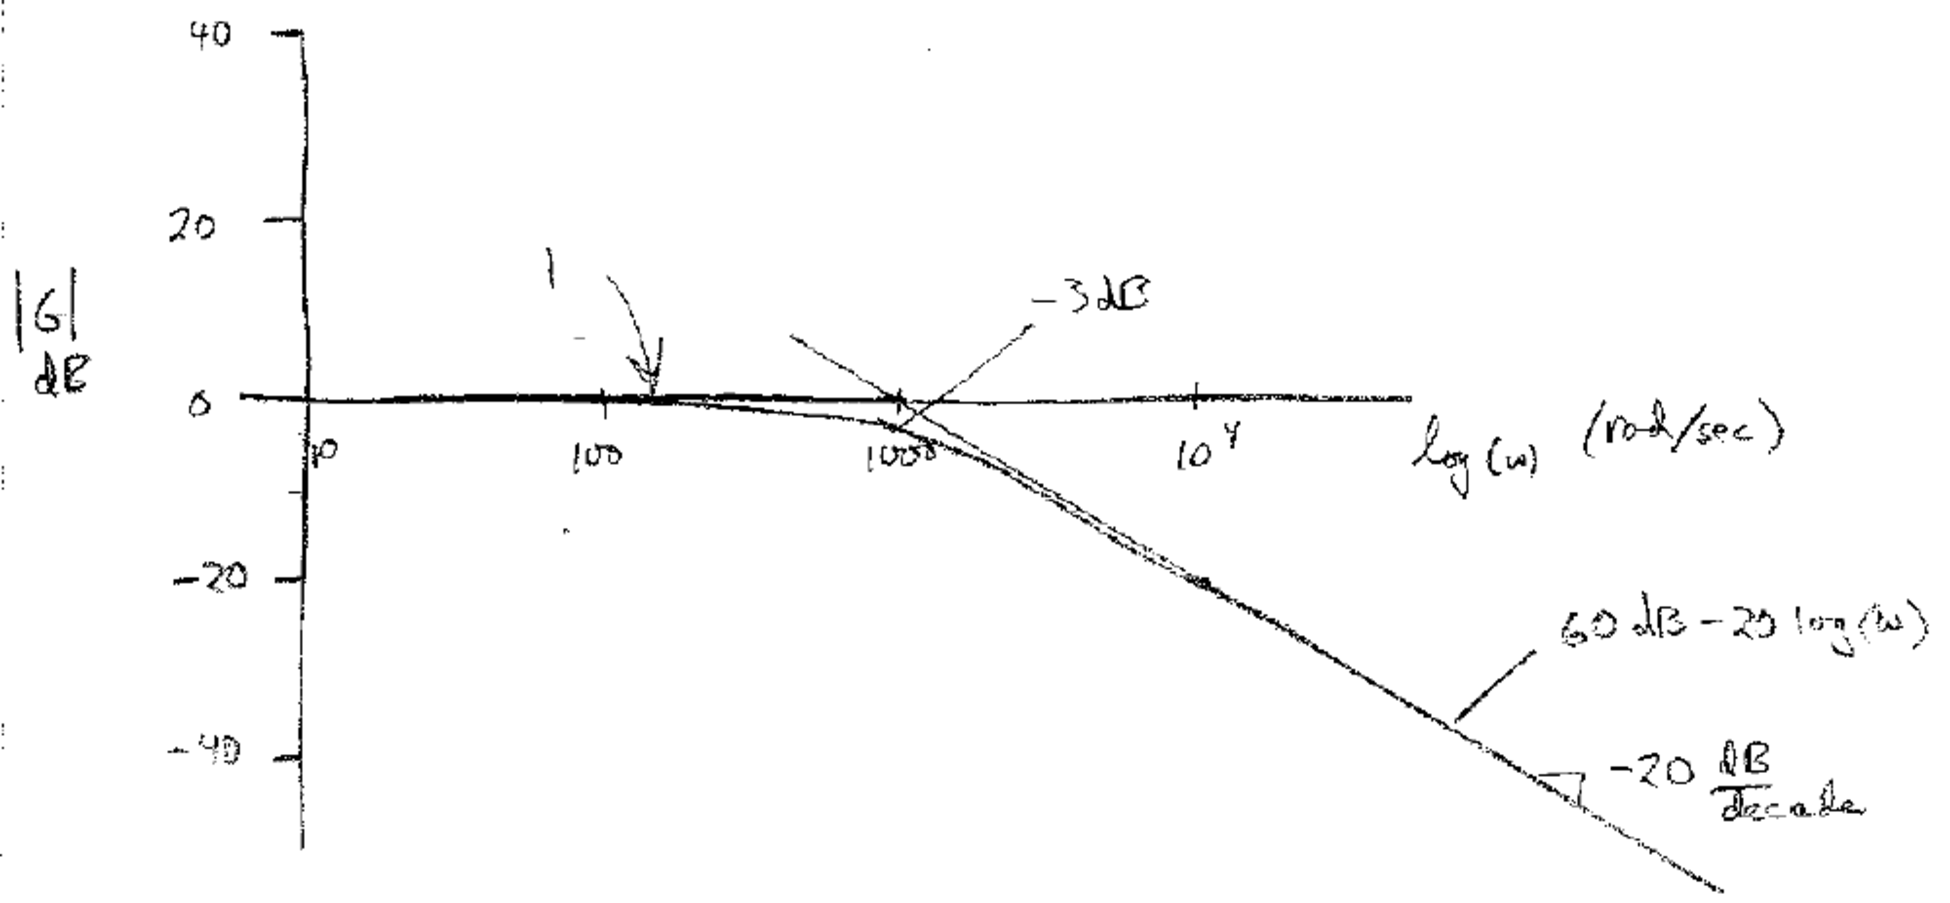
\includegraphics[width=6.5in]{00949a.png}

\paragraph{Angle/Phase:} (slow beginner method)

\[
\omega<<1000 \qquad \angle{G(j\omega)} \approx \angle{\frac{1000}{1000}} = 0^\circ
\]
\[
\omega>>1000 \qquad \angle{G(j\omega)} \approx \angle{\frac{1000}{j\omega}} = -90^\circ
\]
\[
\omega=1000 \qquad \angle{G(j\omega)}    =   \angle{\frac {1} {1+j}}= -45^\circ
\]

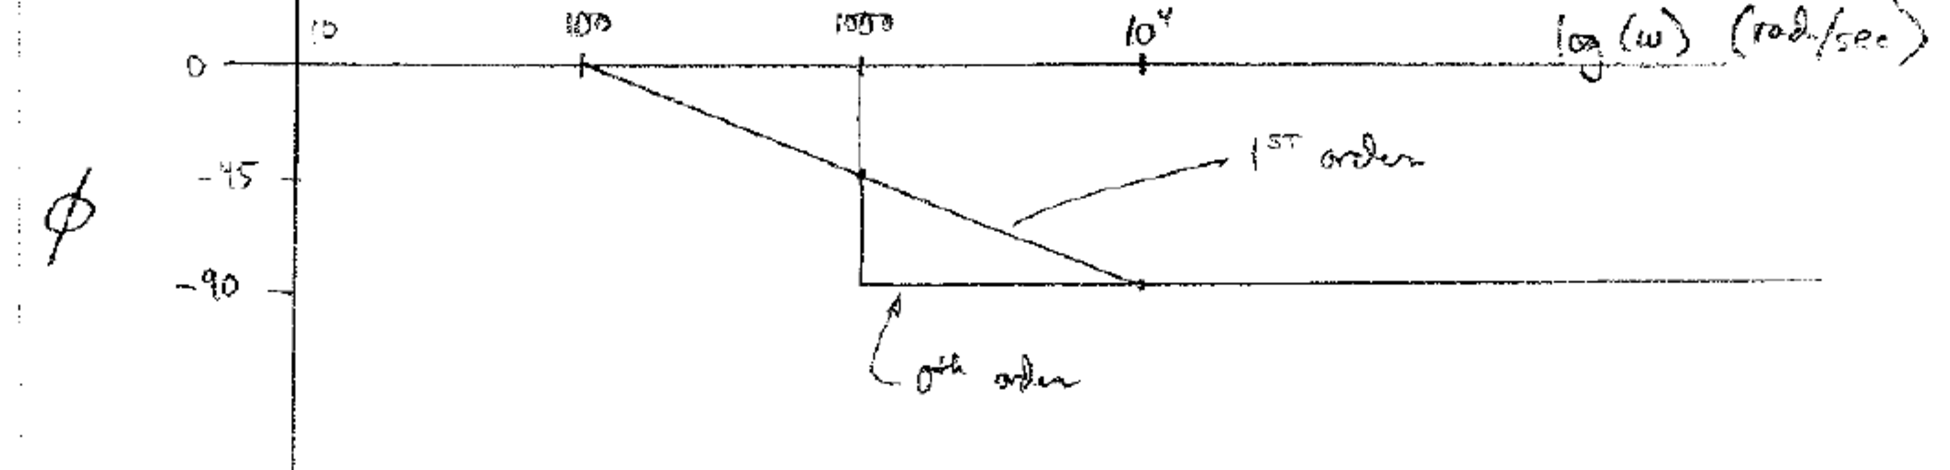
\includegraphics[width=6.5in]{00950a.png}

\end{solution}
	%<*>

%\end{frame}  %%%%%%%%%%%%%%%%%%%%%%%%%%%%%%%%%%%%%%%%%%%%%%%%%%%%%%%%%%%%


	%<*>
%%%%** Section 4.4
\subsection{}

Draw the Bode magnitude and phase plots of
\[
G(s) = \frac{(s+316)}{316}
\]


	%<*n>
\begin{solution}
Fast method:   Recognize that this system consists of a zero.  Remember a zero has an asymptote which ``breaks upward" at the frequency of the zero:

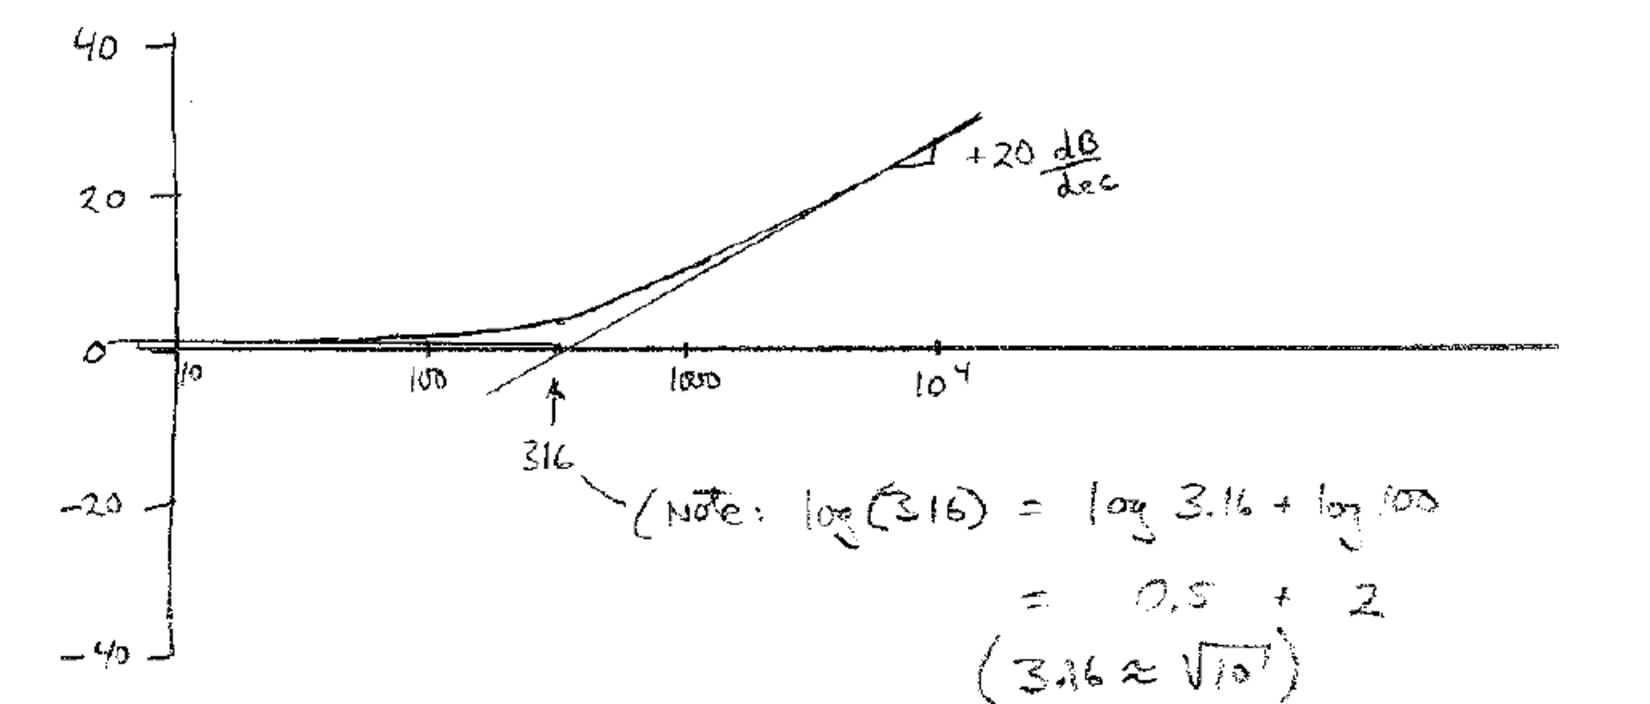
\includegraphics[width=5.5in]{00951a.png}

For phase, the ``0th order" asymptote is a step function from 0 to $+90^\circ$ at the zero frequency, and the 1st order asymptote goes through $+45^\circ$ with a slope of $45^\circ/dec$:

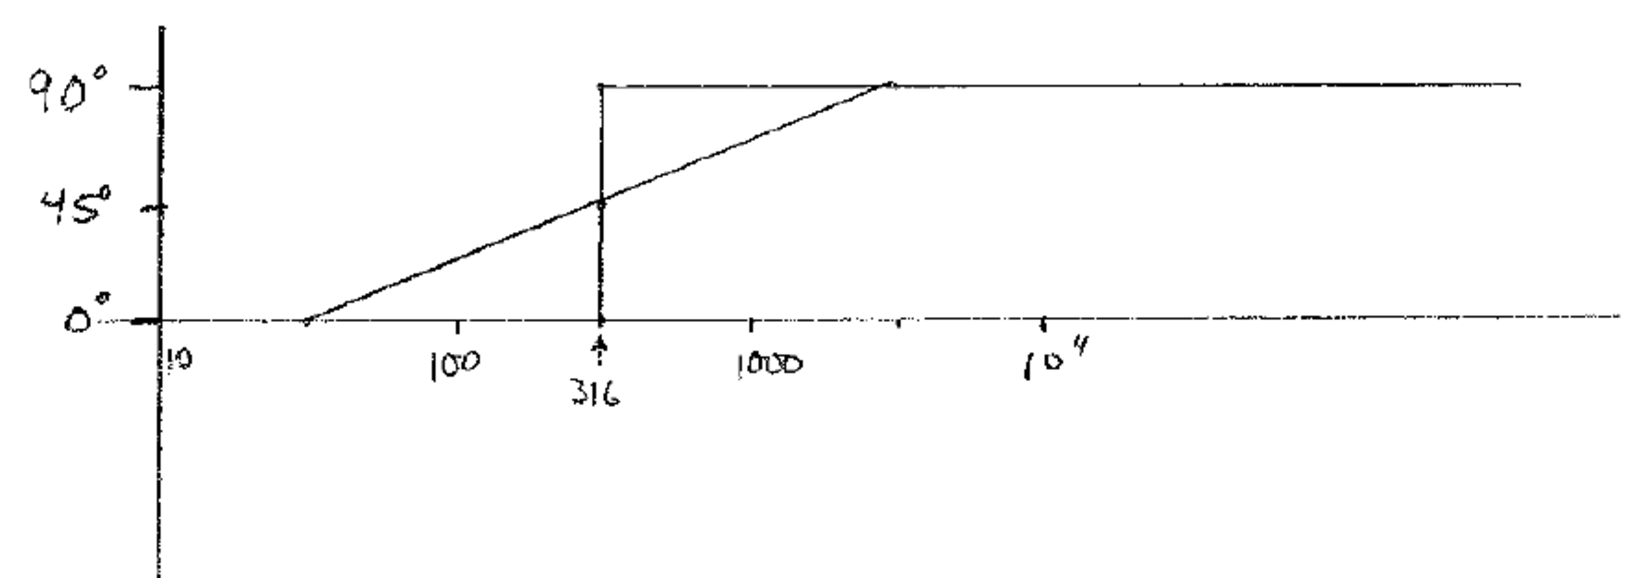
\includegraphics[width=5.5in]{00952a.png}

These results can also be archieved by carefully computing magnitude and phase for the three frequency ranges:
\[
\omega << 316, \qquad \omega = 316, \qquad \omega >> 316
\]

\end{solution}
	%<*>

%\end{frame}  %%%%%%%%%%%%%%%%%%%%%%%%%%%%%%%%%%%%%%%%%%%%%%%%%%%%%%%%%%%%


	%<*>
%%%%** Section 4.5
\subsection{}
Draw the Bode magnitude and phase plots of
\[
G(s) = \frac{3.16\times10^4(s+1)}{(s+31.6)(s+1000)}
\]

	%<*n>
\begin{solution}
Tohelp with the plotting ranges: lowest pole/zero = 1, highest pole/zero = 1000 therefore plot forces
\[
0.1 < \omega < 10^4
\]
For magnitude, evaluate magnitude when $s << 1$(the lowest pole/zero).   In this case evaluate for $s=0$:
\[
|G(j0)| = \frac {1\times 3.16\times 10^4} {31.6\times1000} = 1 = 0dB
\]


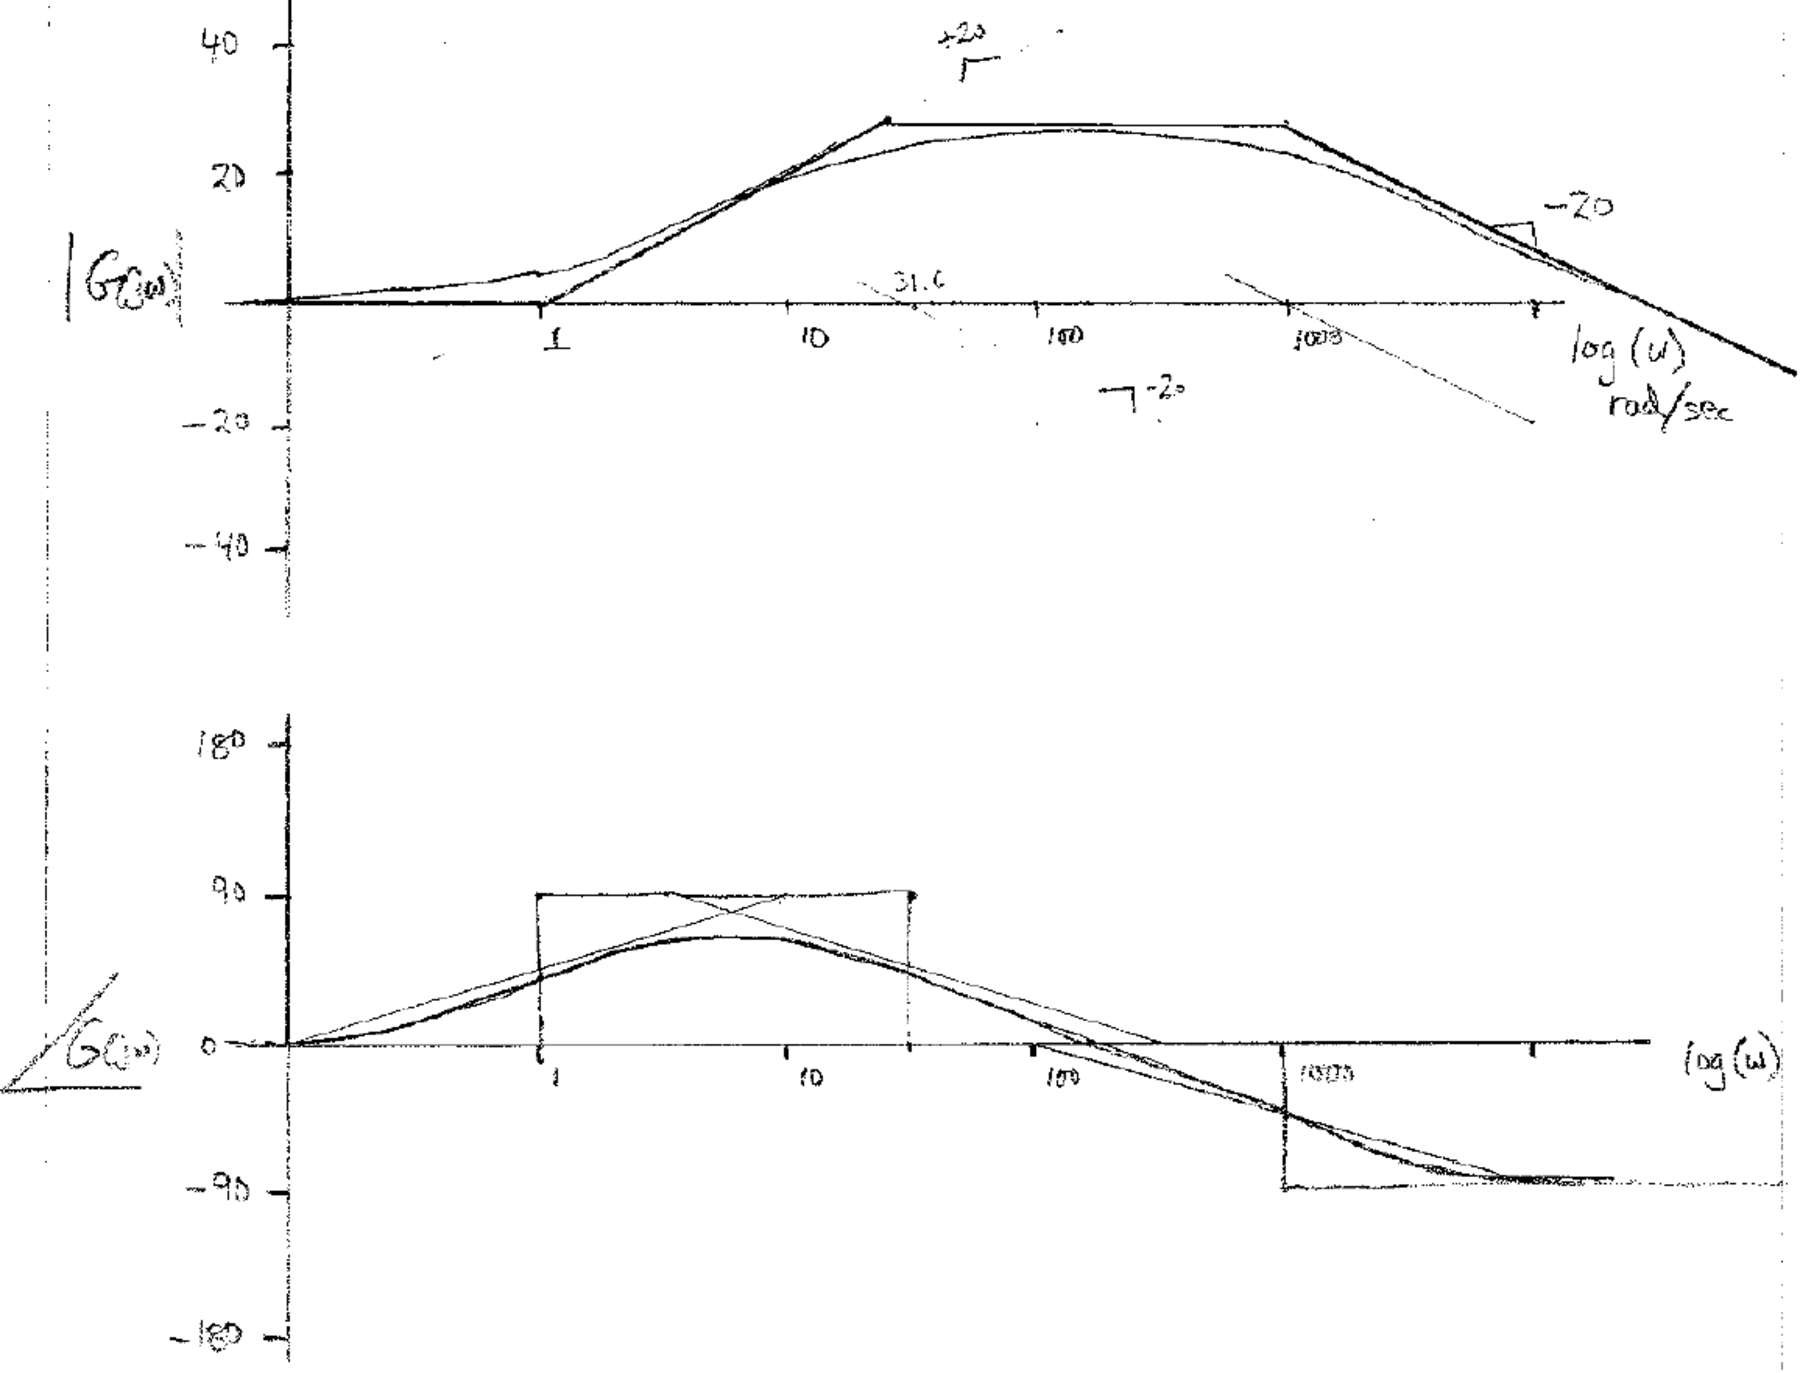
\includegraphics[width=6.0in]{00953a.png}

\end{solution}
	%<*>


%\end{frame}  %%%%%%%%%%%%%%%%%%%%%%%%%%%%%%%%%%%%%%%%%%%%%%%%%%%%%%%%%%%%




	%<*>
%%%%** Section 4.6
\subsection{}
Draw the Bode magnitude and phase plots of
\[
G(s) = \frac{1000}{s^2 + 63.2\zeta s + 1000}
\]
for
\[
\zeta = \{1.0, 0.5, 0.1\}
\]


	%<*n>
\begin{solution}
$\omega_n = \sqrt{1000} = 31.6$

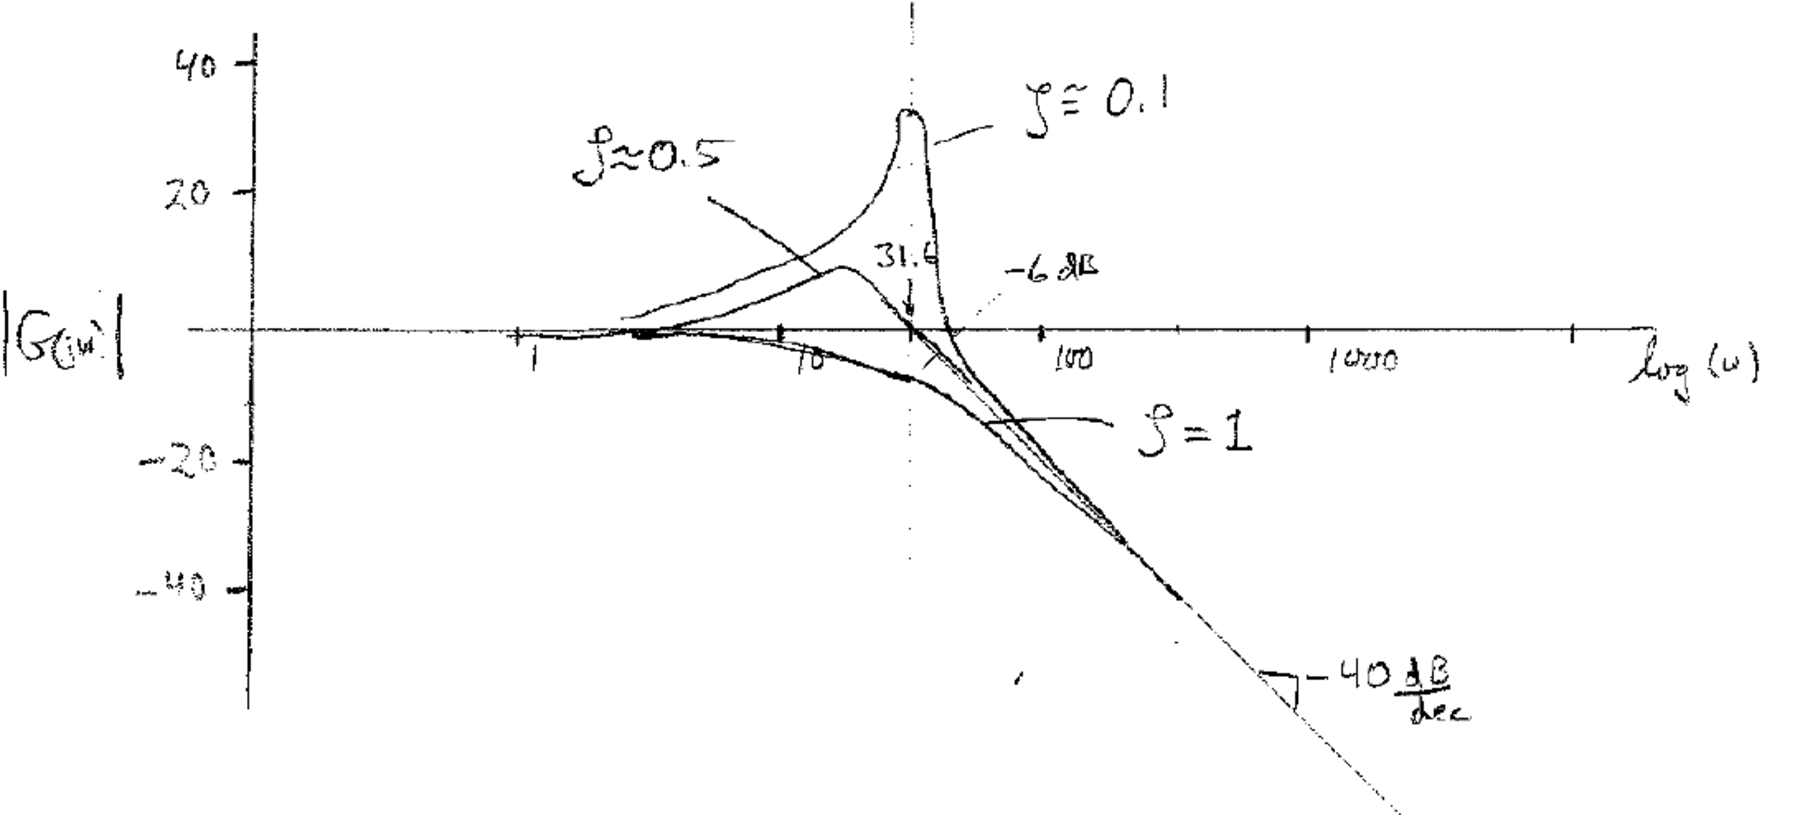
\includegraphics[width=6.0in]{00954a.png}

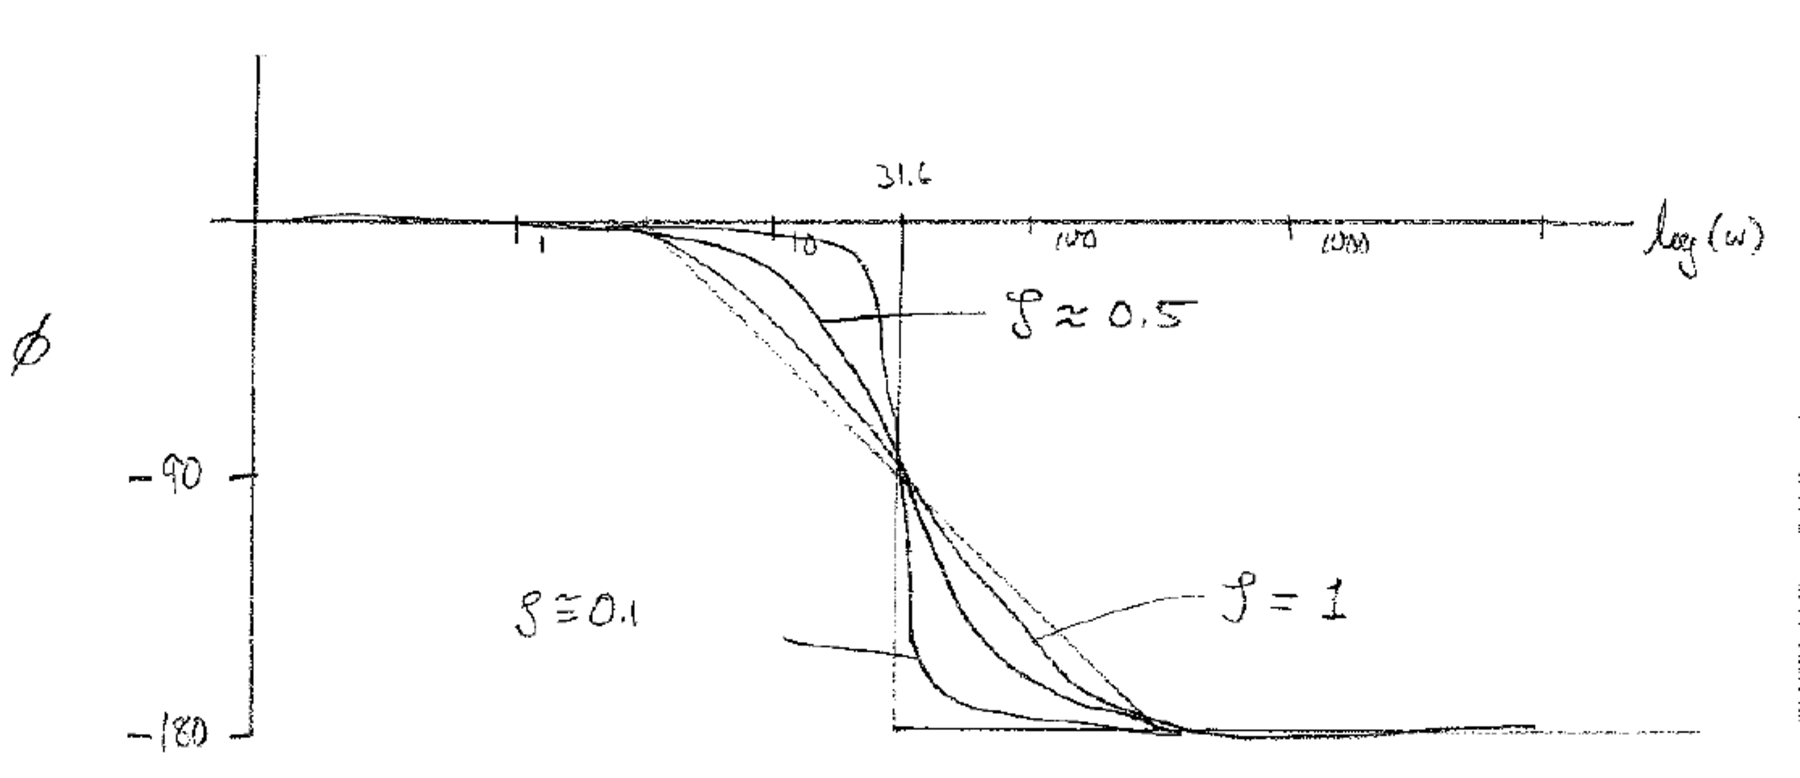
\includegraphics[width=6.0in]{00955a.png}


\end{solution}
	%<*>

%\end{frame}  %%%%%%%%%%%%%%%%%%%%%%%%%%%%%%%%%%%%%%%%%%%%%%%%%%%%%%%%%%%%



	%<*>
%%%%%%%%%%%%%%%%%%%%%%%%%%%%%%%%%%%%%%%%%%%%%%%%%%%%%%%%%%%%%%%%%%%%%%%%%%%%%%%%%%%%%%%%%%%%%%%%%%%%%%%%%%
\newpage
%%%%** Section 5 
\section{EE447 In Class Problems: Closed Loop Feedback}

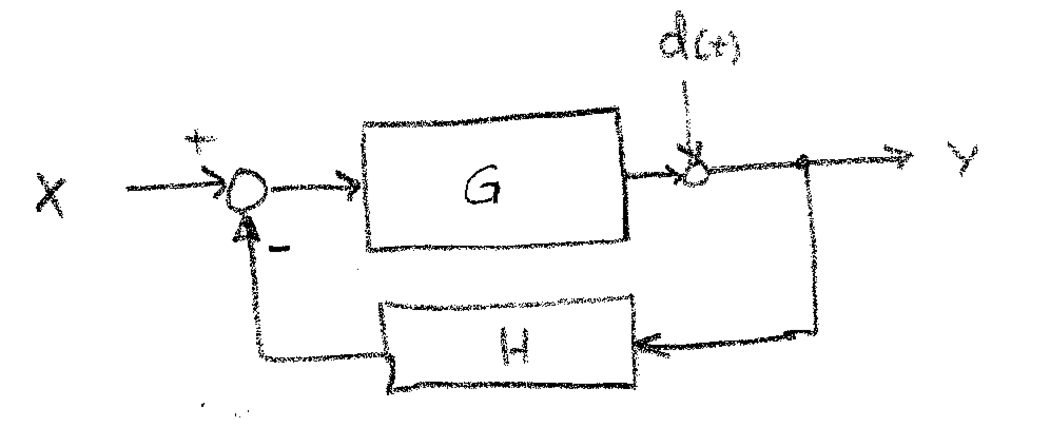
\includegraphics[width=3.5in]{00388a.png}

(ICPs 5.1 --- 5.4 refer to this diagram:)

%%%%** Section 5.1
\subsection{}\label{disturbancerej1}

Find $\frac{Y(s)}{d(s)}$ for $G=100, H=2, X = 0$. \\[0.15in]

	%<*n>
\begin{solution}
\[
\frac{Y}{d} = \frac{1}{1+GH} = \frac{1}{201} = 0.004975
\]
\end{solution}
	%<*>


%%%%** Section 5.2
\subsection{}
For the system in \ref{disturbancerej1}, find
$\frac{Y}{X}$ for d(t) = 0 (D(s) = 0), and find
$\frac{Y}{d}$ for $X(s) = 0$.

Compute both for $G = 90, 100, 110$ and $H=2$.\\[0.15in]

	%<*n>

\begin{solution}
\begin{tabular}{c|c|c|c}
$|G|$   		&  $\frac{G}{1+GH}$      &  $Y/X$   	&  $Y/d$\\ \hline
90		&  $\frac{90}{1+180}$    &  0.4972      &  0.005524  \\
100             &  $\frac{100}{201}$	 &  0.4975	&  0.004975 \\
110             &  $\frac{110}{220}$	 &  0.4977      &  0.004525
\end{tabular}
\end{solution}







	%<*>
%%%%** Section 5.3
\subsection{}
 From the results of \ref{disturbancerej1}, find the sensitivity coefficients for the performance measures $P_1=|\frac{Y}{X}|$ and $P_2=|\frac{Y}{d}|$with respect to the parameter $p_1 = G$?\\[0.15in]

	%<*n>
\begin{solution}


Taking the last two rows of the table, $\Delta p_1 = 110-100 = 10$.
\[
S_{11} = \frac{\Delta P_1/P_1}{\Delta p_1/p_1} = \frac{(0.4977-0.4975)/0.4975}{10/100} = 0.00402 = 0.4\%
\]
\[
S_{21} = \frac{\Delta P_2/P_2}{\Delta p_1/p_1} = \frac{(0.004525-0.004975)/0.004975}{10/100} = -90.5\%
\]
Notice that the disturbance rejection is much more sensitive to $|G|$ than the closed loop gain!

\end{solution}
	%<*>



	%<*>
%%%%** Section 5.4
\subsection{} For $G = \frac{500}{s+270}, H=1$, find disturbance gain $\frac{Y(s)}{d(s)}$ for $X(s)=0$.  Sketch Bode Magnitude Plot of $GH(s)$ and $\frac{Y(s)}{d(s)}$ on the same axes.

	%<*n>
\begin{solution}
\[
R(s) = \frac{Y(s)}{d(s)} = \frac{1}{1+500/(s+270)} = \frac{(s+270)}{(s+770)}
\]
Because we assume $X(s)=0$.
Note that system looses its ability to reject disturbance completely when $|GH| = 1 = 0dB$.

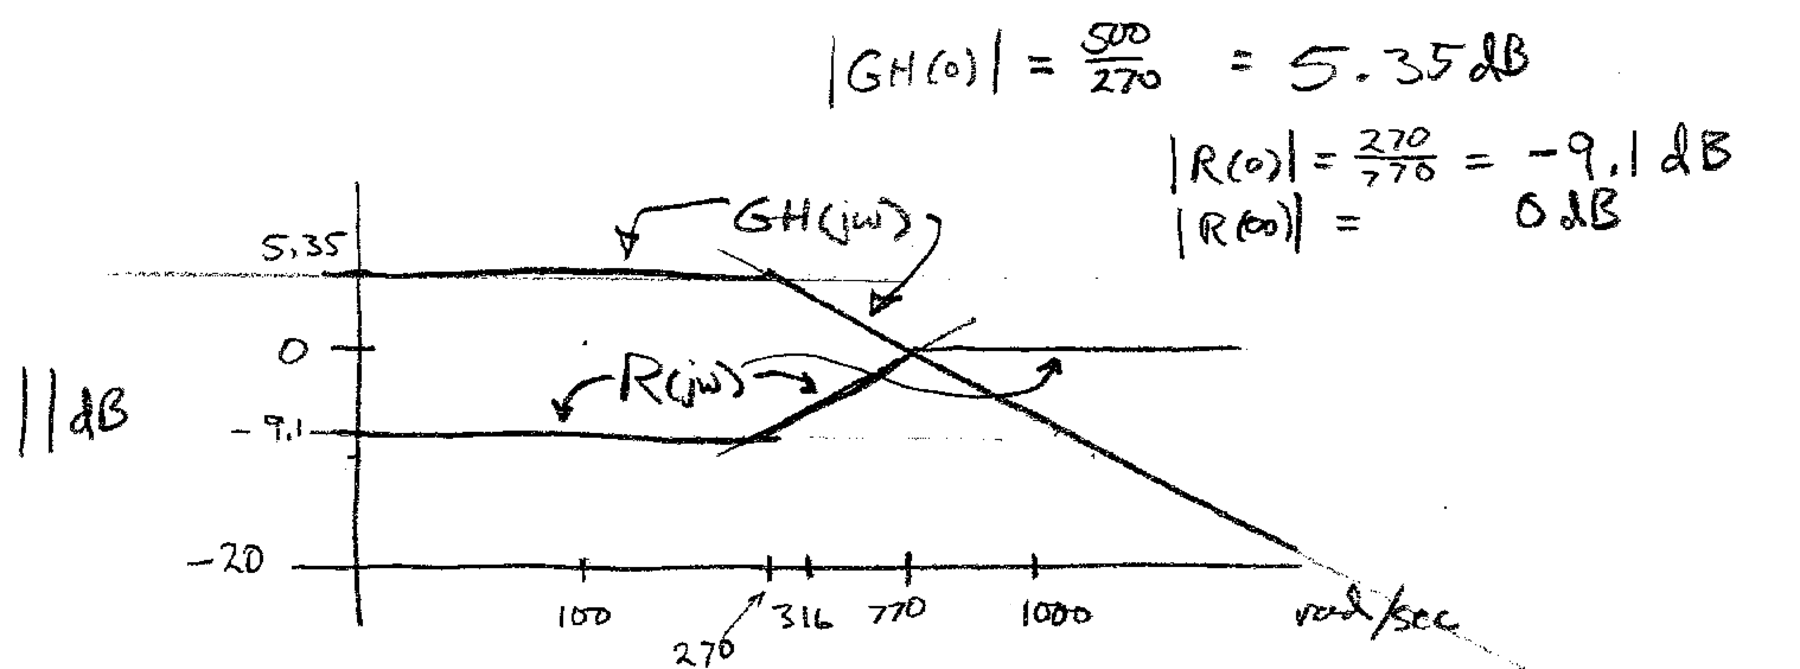
\includegraphics[width=6.0in]{00564a.png}
\end{solution}


	%<*>

	%<*>
%%%%** Section 5.5
\subsection{}
 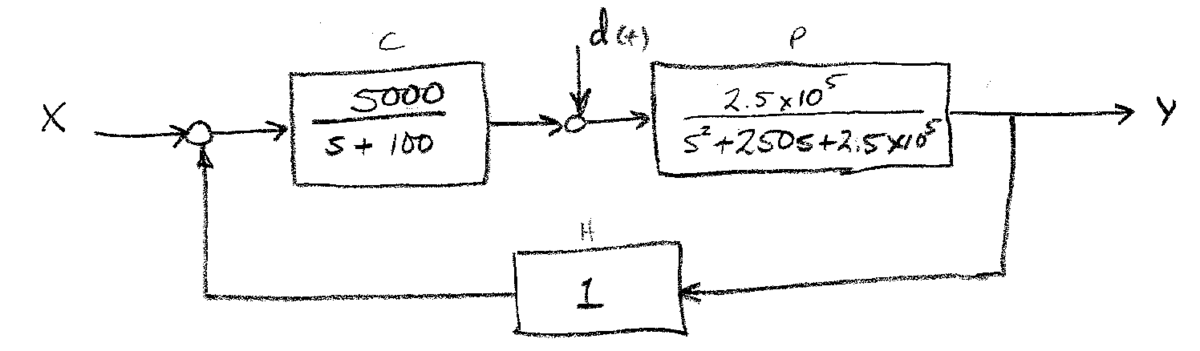
\includegraphics[width=4.0in]{00470a.png}

A) Find $\frac{Y(s)}{d(s)}$ assuming $CPH>>1$. Make a Bode magnitude plot of $|Y(s)/d(s)|$.
On the same axes, make a Bode Magnitude plot of $CPH(s)$.

B) For what range of frequencies is the loop gain magnitude $>1$?

C) What do you notice about the relationship between $CPH(s)$ and $\frac{Y(s)}{d(s)}$?

	%<*n>
\begin{solution}
\[
Y(s) = \frac{CP}{1+CPH}X(s) + \frac{P}{(1+CPH)}d(s) = \frac{P}{(1+CPH)}d(s)
\]
for $|CPH|>>1$,
\[
Y(s)/d(s) = \frac{(s+100)}{(5000)}
\]
For
\[
\omega << 100, \qquad \left | \frac {Y(j\omega)} {d(j\omega)} \right | \approx 0.020
\]
For
\[
\omega = 100, \qquad \left | \frac {Y(j\omega)} {d(j\omega)} \right | \approx 0.028
\]
For
\[
\omega >> 100, \qquad \left | \frac {Y(j\omega)} {d(j\omega)} \right | \approx \frac{\omega}{500}
\]

But, we need to check our assumption that $|CPH(j\omega)|>>1 $.  We'll make the Bode Mag. plot to see where it crosses $0dB$. In fact,
\[
|CPH| = |\frac{5000\times2.5\times10^5}{(s+100)(s^2+250s+2.5\times10^5)}|
\]
We get, $\omega_n = \sqrt{2.5\times10^5} = 500$.

For
\[
\omega << 100 \qquad |CPH| = 50 = 34dB
\]
Making the Bode Magnitude plot of $|CPH(j\omega)|$,  There is a pole at 100, and a second order pole with light damping ($\zeta=0.25$) at $\omega = 500$.

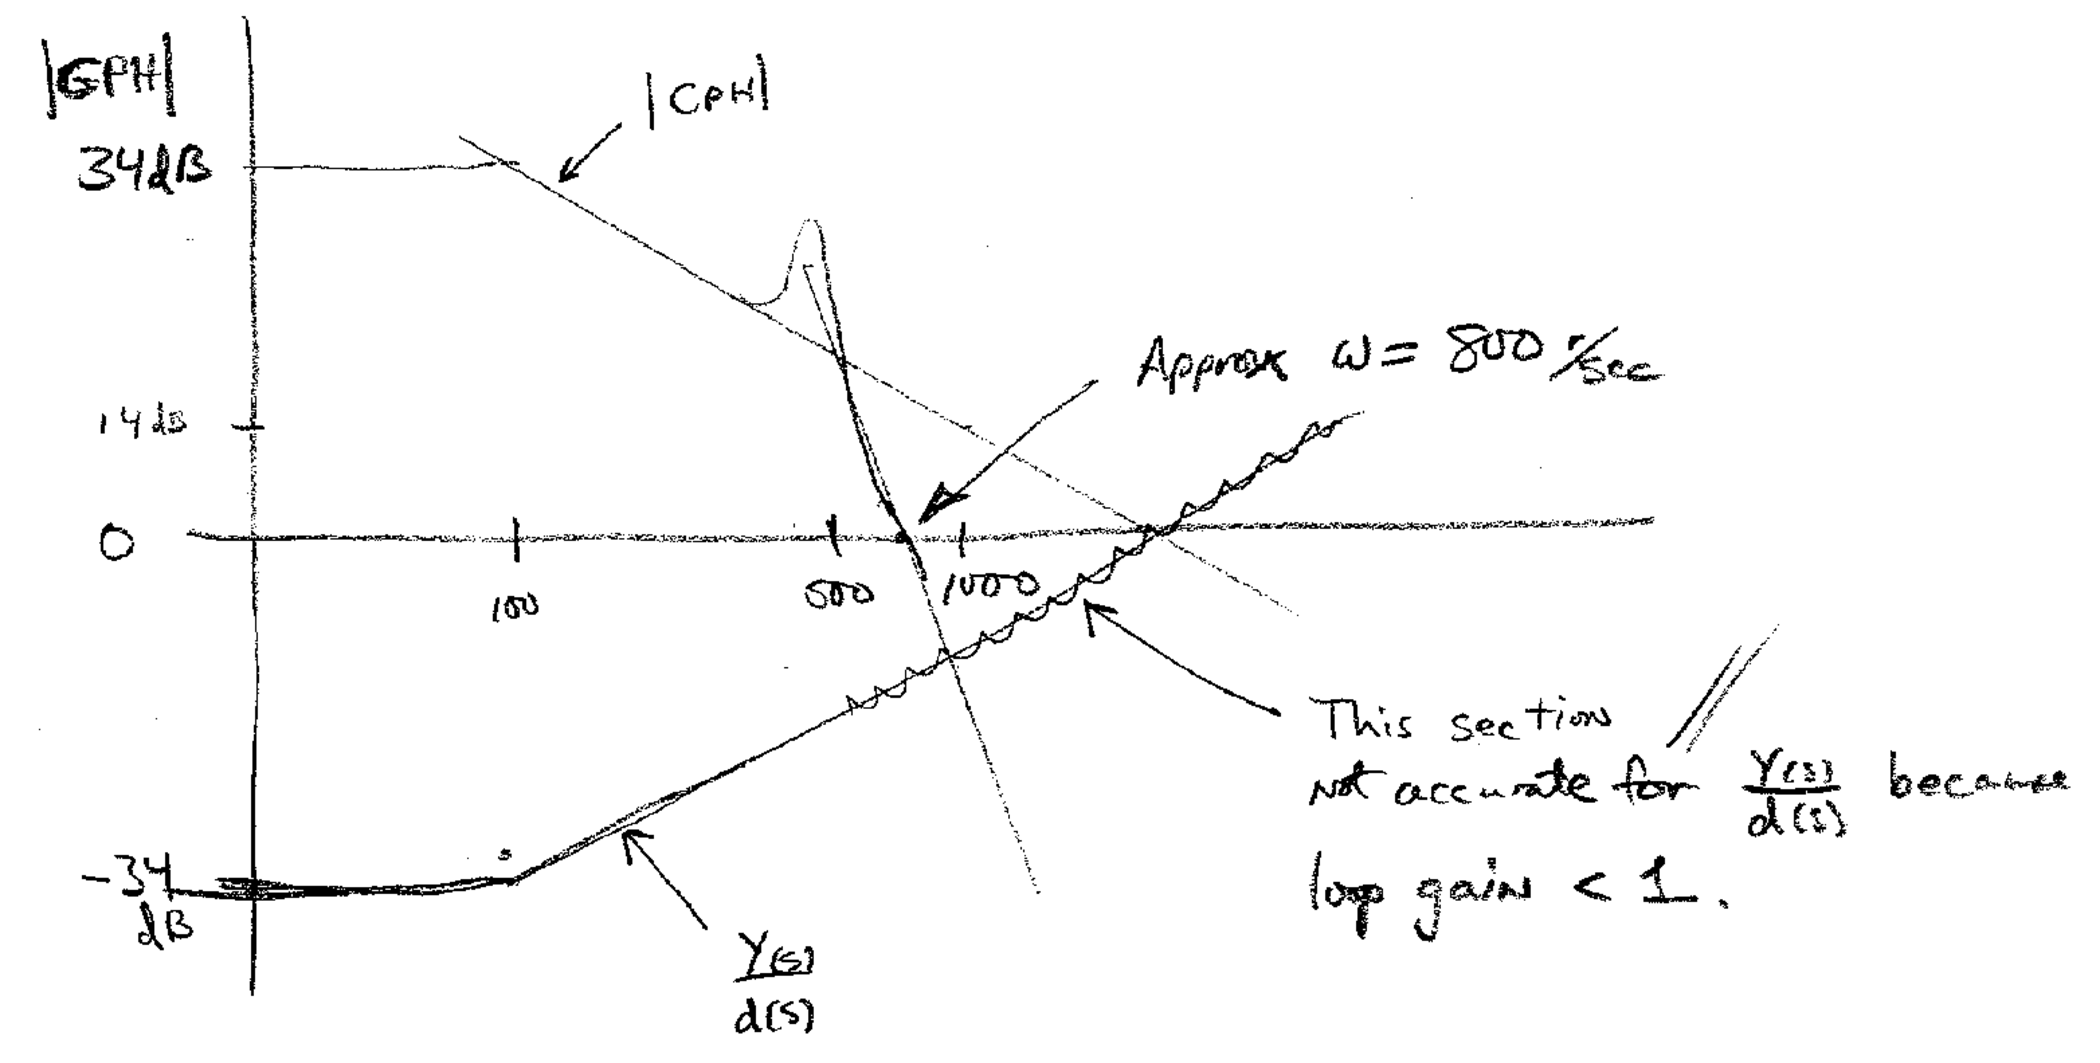
\includegraphics[width=7.0in]{00565a.png}


As with 5.4, note that the system looses its ability to reject disturbance completely when $|GH| = 1 = 0dB$.


Let's check our Bode plots with Scilab (pls see {\tt icp5\_5.sce}).

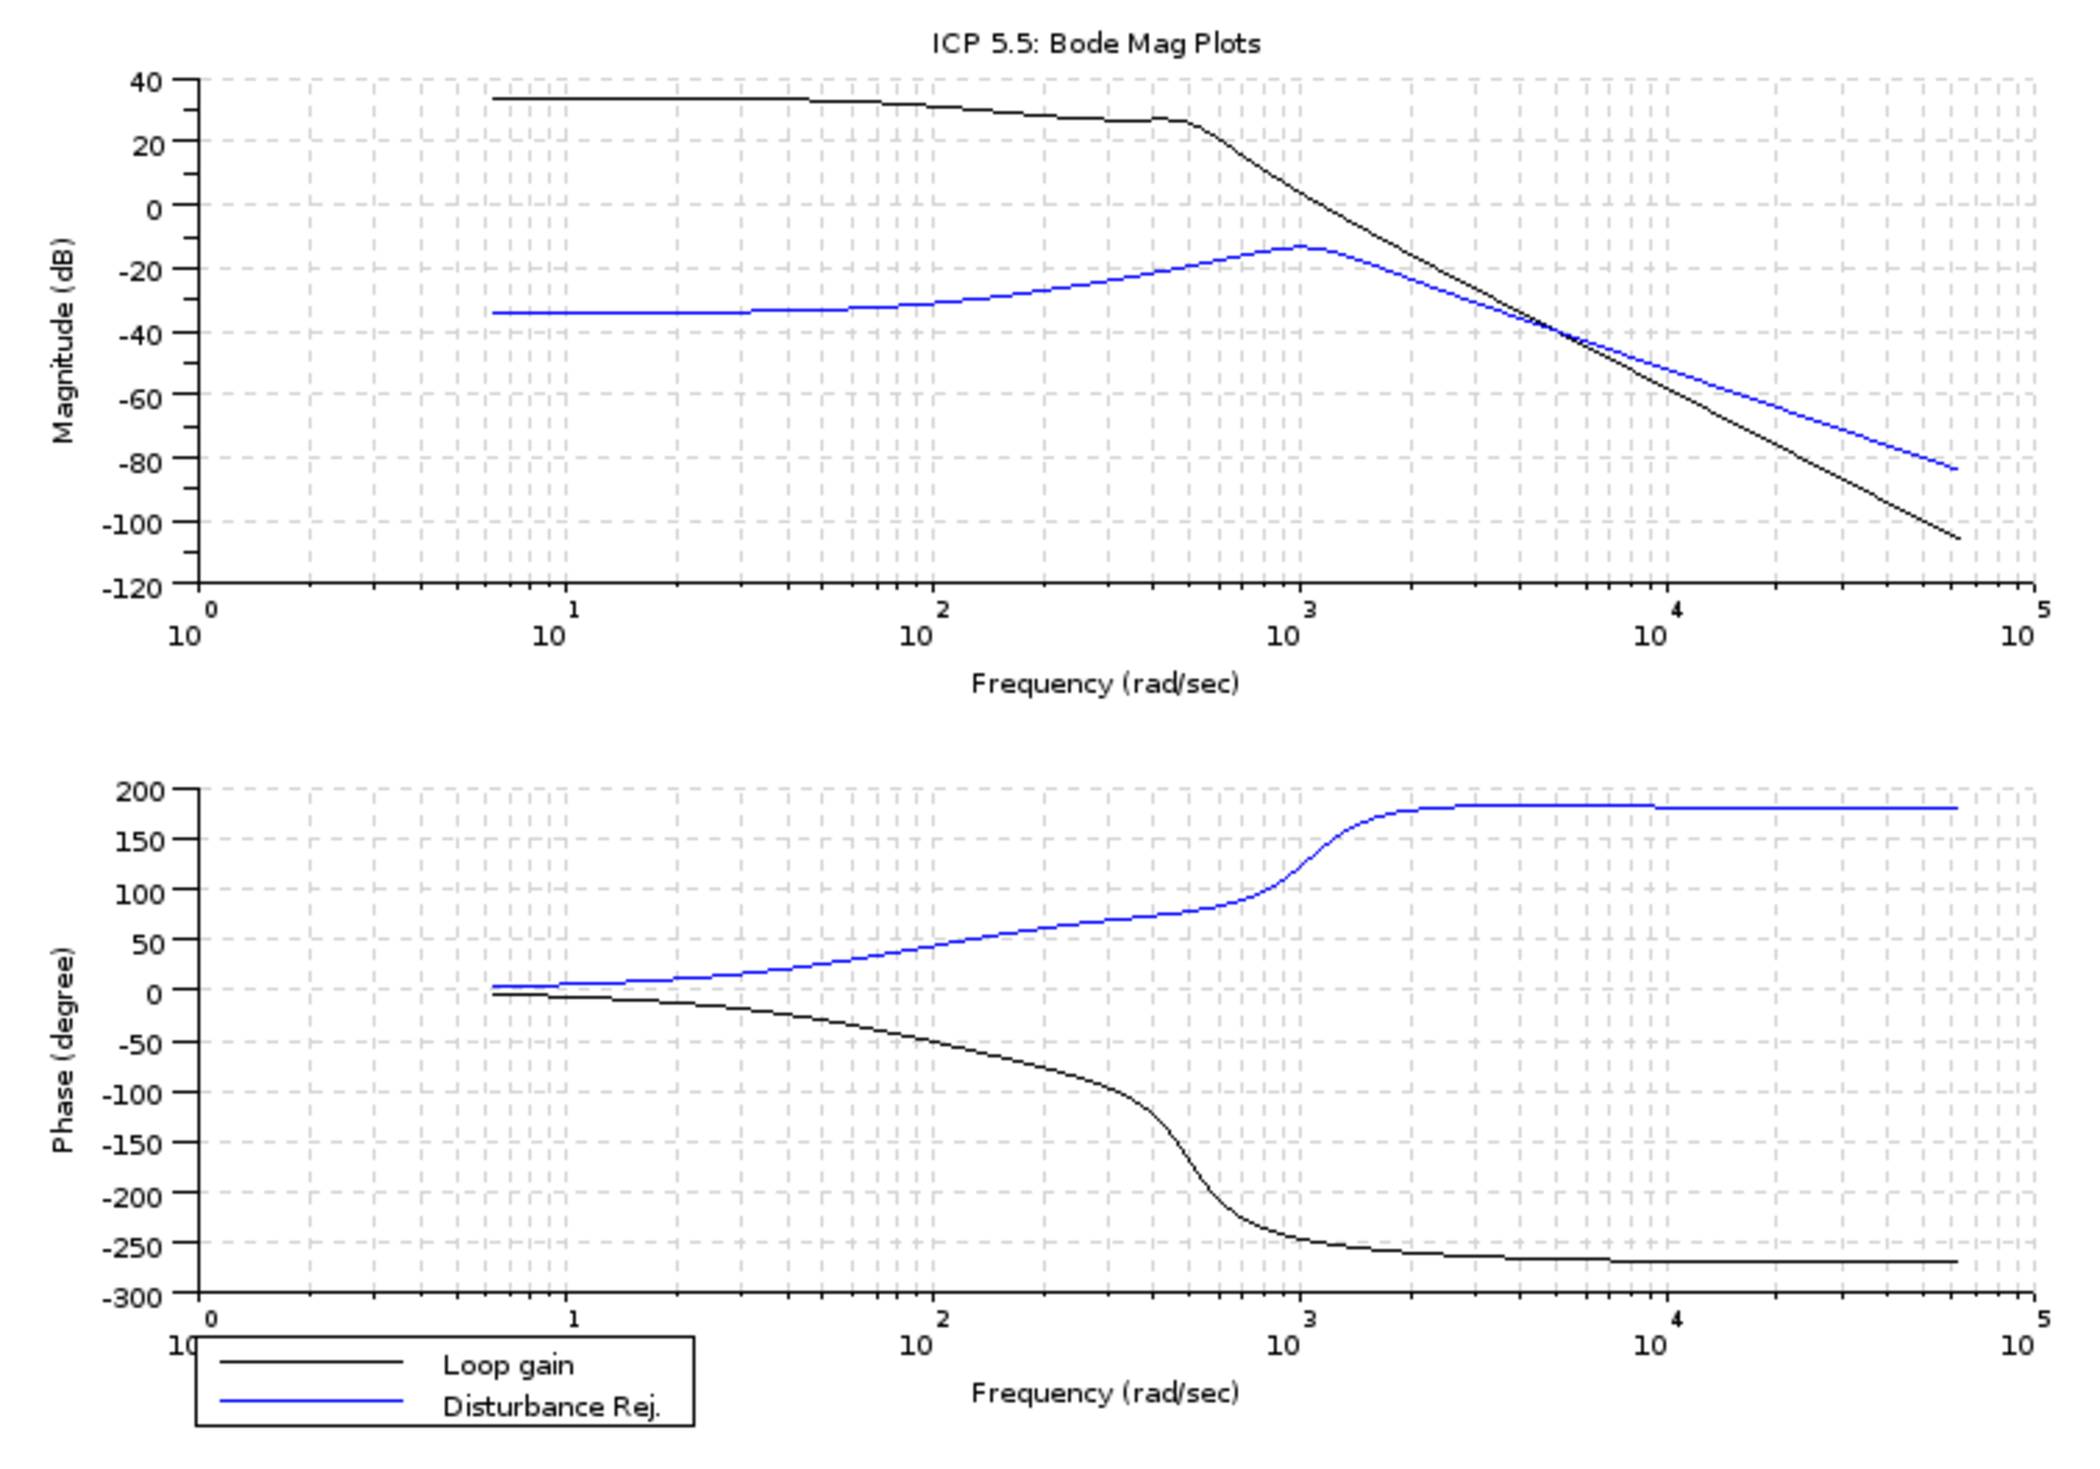
\includegraphics[width=7.0in]{icp5_5_bodea.png}

{\bf Notes: }

1) Disturbance rejection deviates from prediction above about 1000rad/sec due to violation of $CPH>>1$ assumption above 1000 rad/sec.

2) 2nd order peak in loop gain ($CPH(s)$) seems less prominent (visible) in this plot because the vertical scale is very large.

3) Further analysis with scilab shows that this system is quite unstable!  (We'll tackle that next week).

4) My value of $\omega$ where $|CPH(j\omega)| = 0$ was off because I didn't follow my own rule:  {\it make the y axis scale such that the vertical size of $20dB$ is equal to the horizontal size of a factor of 10!}. (The computer can get an accurate plot without following that rule !@\#*!@\#\_\$*\&).

\end{solution}

	%<*>
%%%%** Section 5.6
\subsection{}

\begin{center}
%%%%%%%%%%%%%%%%%%%%%%%%%%%%%%%%%%%%%%%%%%%%%%%%%%%%%%%%%%%%%%%%%%%%%%%%%%%%%%%%%%%%%%%%

%        Closed loop control system

%%%%%%%%%%%%%%%%%%%%%%%%%%%%%%%%%%%%%%%%%%%%%%%%%%%%%%%%%%%%%%%%%%%%%%%%%%%%%%%%%%%%%%%%

\begin{tikzpicture}[every node/.style={draw, thick,outer sep=0pt,thick}]

% %
% debugging grid
%  \draw[step=5mm,gray,very thin] (-25mm,-25mm) grid (100mm,50mm);
%  \draw[thick,gray] (0,-25mm) -- (0,50mm);
%  \draw[thick,gray] (-25mm,0) -- (100mm,0);
%
%
%

 \node (C) [thick,minimum width=14mm, minimum height=10mm] {$\frac{1000}{s+\rho}$};
 \node (H) [thick, yshift=-10mm] {$H=1$};

 \coordinate (outend) at ($(C.east)+(12.5mm,0)$);
 \coordinate (out2)   at ($(C.east)+(5mm,0)$);
 \draw [->] (C.east) -- (outend);
 \draw [->]  (out2)   -- ++(0,-10mm) -- (H.east);

 \node (sum)   [circle,draw,minimum width=0.1cm ] at (-12.5mm,0mm) {};

 \draw [->] (H.west) -- (-12.5mm,-10mm) -- (sum.south);

 \draw [->] (sum.east) -- (C.west);
 \draw [<-] (sum.west) -- ++(-5mm,0mm);

\tikzstyle{every node}=[];

 \coordinate  (input) at ($(sum.west)+(-5mm,0)$) node[xshift=-25mm] {$X(s)$};

 \node (output) at ($(outend)+(5mm,0mm)$) {$Y(s)$};

% \draw [thick] (Mc.east)  --  (Xa);

\end{tikzpicture}
%        Closed loop control system (end)

%%%%%%%%%%%%%%%%%%%%%%%%%%%%%%%%%%%%%%%%%%%%%%%%%%%%%%%%%%%%%%%%%%%%%%%%%%%%%%%%%%%%%%%%
\end{center}

A) Let $\rho$ take on the values \{90, 100, 110\}.  What is the 3dB frequency, $\omega_{3dB}$ of the closed loop transfer function $\frac{Y(s)}{X(s)}$ for each value of $\rho$.?

	%<*n>
\begin{solution}
\[
\frac{Y(s)}{X(s)} = \frac{G}{1+GH} = \frac{1000/(s+\rho)}{1+1000/(s+\rho)} = \frac{1000}{s+\rho+1000}
\]
\begin{tabular}{c|c|c}
$\rho$		&  $Y(s)/X(s)$		& $\omega_{3dB}$        \\ \hline
90		&  $\frac{1000}{s+1090}$	& 1090       \\
100             &  $\frac{1000}{s+1100}$	& 1100		\\
110             &  $\frac{1000}{s+1110}$        & 1110
\end{tabular}
\end{solution}
	%<*>

B) What is the sensitivity coefficient  of $\omega_{3dB}$ with respect to $\rho$?

	%<*n>
\begin{solution}
\[
S_{ij} = \frac  {\frac{\Delta\omega_{3dB}}  {1100} } {\frac{\Delta\rho}{100}} = 
\frac {\frac{10}{1100}} {\frac{10}{100}} 
= \frac{10\times100}{10\times 1100} = 0.09 = 9\%
\]
\end{solution}
	%<*>


	%<*>
%%%%** Section 5.7
\subsection{}
 Referring back to the first block diagram (Prob \ref{disturbancerej1}), assume $G=\frac{100}{s+20}$, $H=1$.

A) What is $\frac{Y(s)}{d(s)}$?   Sketch Bode Magnitude Plot.

	%<*n>
\begin{solution}
\[
\frac{Y(s)}{d(s)} = \frac{(s+20)}{(s+120)}
\]
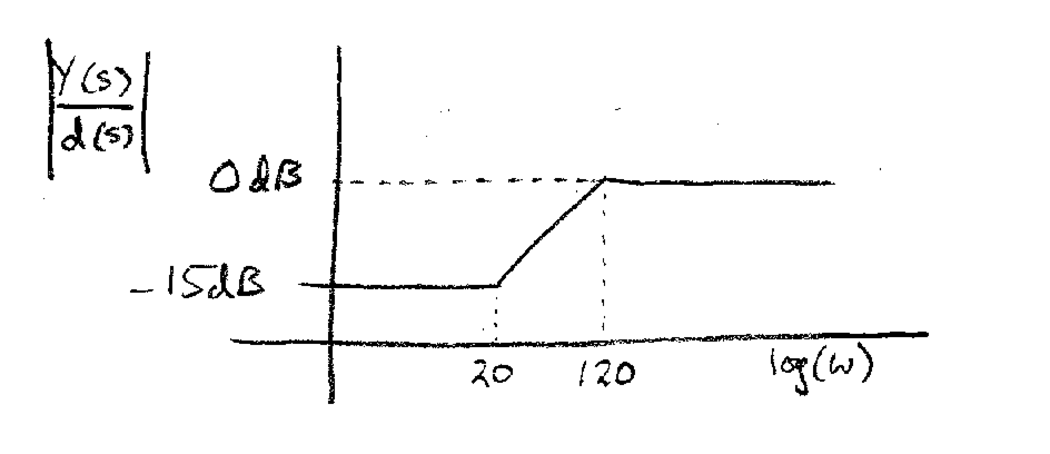
\includegraphics[width=3.5in]{00566a.png}
\end{solution}
	%<*>

B) Evaluate $|\frac{Y(j\omega)}{d(j\omega)}|$ for $\omega = \{1, 500\}$ and $X=0$.

	%<*n>
\begin{solution}
\[
|Y(j1)| = |\frac{(J+20)}{(j+120)} \approx 20/120 = 0.167 = -15dB
\]
\[
|Y(j500)| = |\frac {500j+20} {500j+120} | \approx \frac{500}{514} = 0.973 = -0.24dB
\]

\end{solution}
	%<*>

C) What should you change to reduce disturbance output to about -15dB at $\omega=500$?

	%<*n>
\begin{solution}
There are a number of things you could do, but looking at the Bode plot above, if our frequency of interest was 5 instead of 500 we would already be at $-15dB$.   The parameters we can change are G and H.  One simple change would be to increase the pole of G from 20 to 5000. 

\[
G_2(s) = \frac {100}{s+5000}
\]

    Going a factor of 10 (1 decade) above 500, means that the actual curve will be close to the low-frequency (first horizontal) asymptote, but now the disturbance rejection is no longer  $-15dB$:
    
\[
|R_2(s)|_{s=0} = \left . \frac{s+5000}{s+5100} \right |_{s=0} = 0.9804 = -0.18dB
\]
not nearly enough reduction of the disturbance (we wanted $-15dB$).  Note that the pole of $R(s)$ works out to the {\it sum} of the 
numerator and the pole of the open loop gain ($100 + 5000$).    Let's make the numerator bigger:
 
\[
G_3(s) = \frac {25000}{s+5000}
\]
then 
\[
|R_2(s)|_{s=0} = \left . \frac{s+5000}{s+35000} \right |_{s=0} = -17dB
\]
So our disturbance rejection is even more than $-15dB$.  We can approach this two ways. 1) (preferred) is that $-17dB$ is event {\it better} than $-15dB$ so we are done.  2) If we want to get exact we can solve for the exact numerator (gain):

\[
20 \log_{10}\left( \frac{5000}{x+5000} \right) = -15 \to  \frac{5000} {5000+x} = 10^{\frac{-15}{20}} = 0.1778 \to x = 23121
\]

\end{solution}
	%<*>







%%%%%%%%%%%%%%%%%%%%%%%%%%%%%%%%%%%%%%%%%%%%%%%%%%%%%%%%%%%%%%%%%%%%%%%%%%%%%%%%%%%%%%%%%%%%%%%%%%%%%
\newpage
%%%%** Section 6 
\section{EE447 In Class Problems: Root Locus}

In all Root Locus problems, we are looking for a) correct number of diverging asymptotes, b) correct angles for the asymptotes, c) correct part of the real line occupied by the RL, d) correct intercept of the asymptotes with the real line, e) arrows correctly showing direction of pole movement as $K$ is increased.

%%%%%%%%%%%%%%%%%%%%%%%%%%%%%%%%%%%%%%%%%%%%%%%%%%%%%%%%%%%%%%%%%%%%%%%%%%%%%%%%%%%%%%%%%%%%%%%%%%%%%%%%%
	%<*>
%%%%** Section 6.1
\subsection{}

%%%%** Section 6.1.1 
\subsubsection{}
	%<*>
\label{xx1} Plot the root locus for $K>0$ where
\[
CPH(s) = \frac{K}{(s+10)(s+20)}
\]

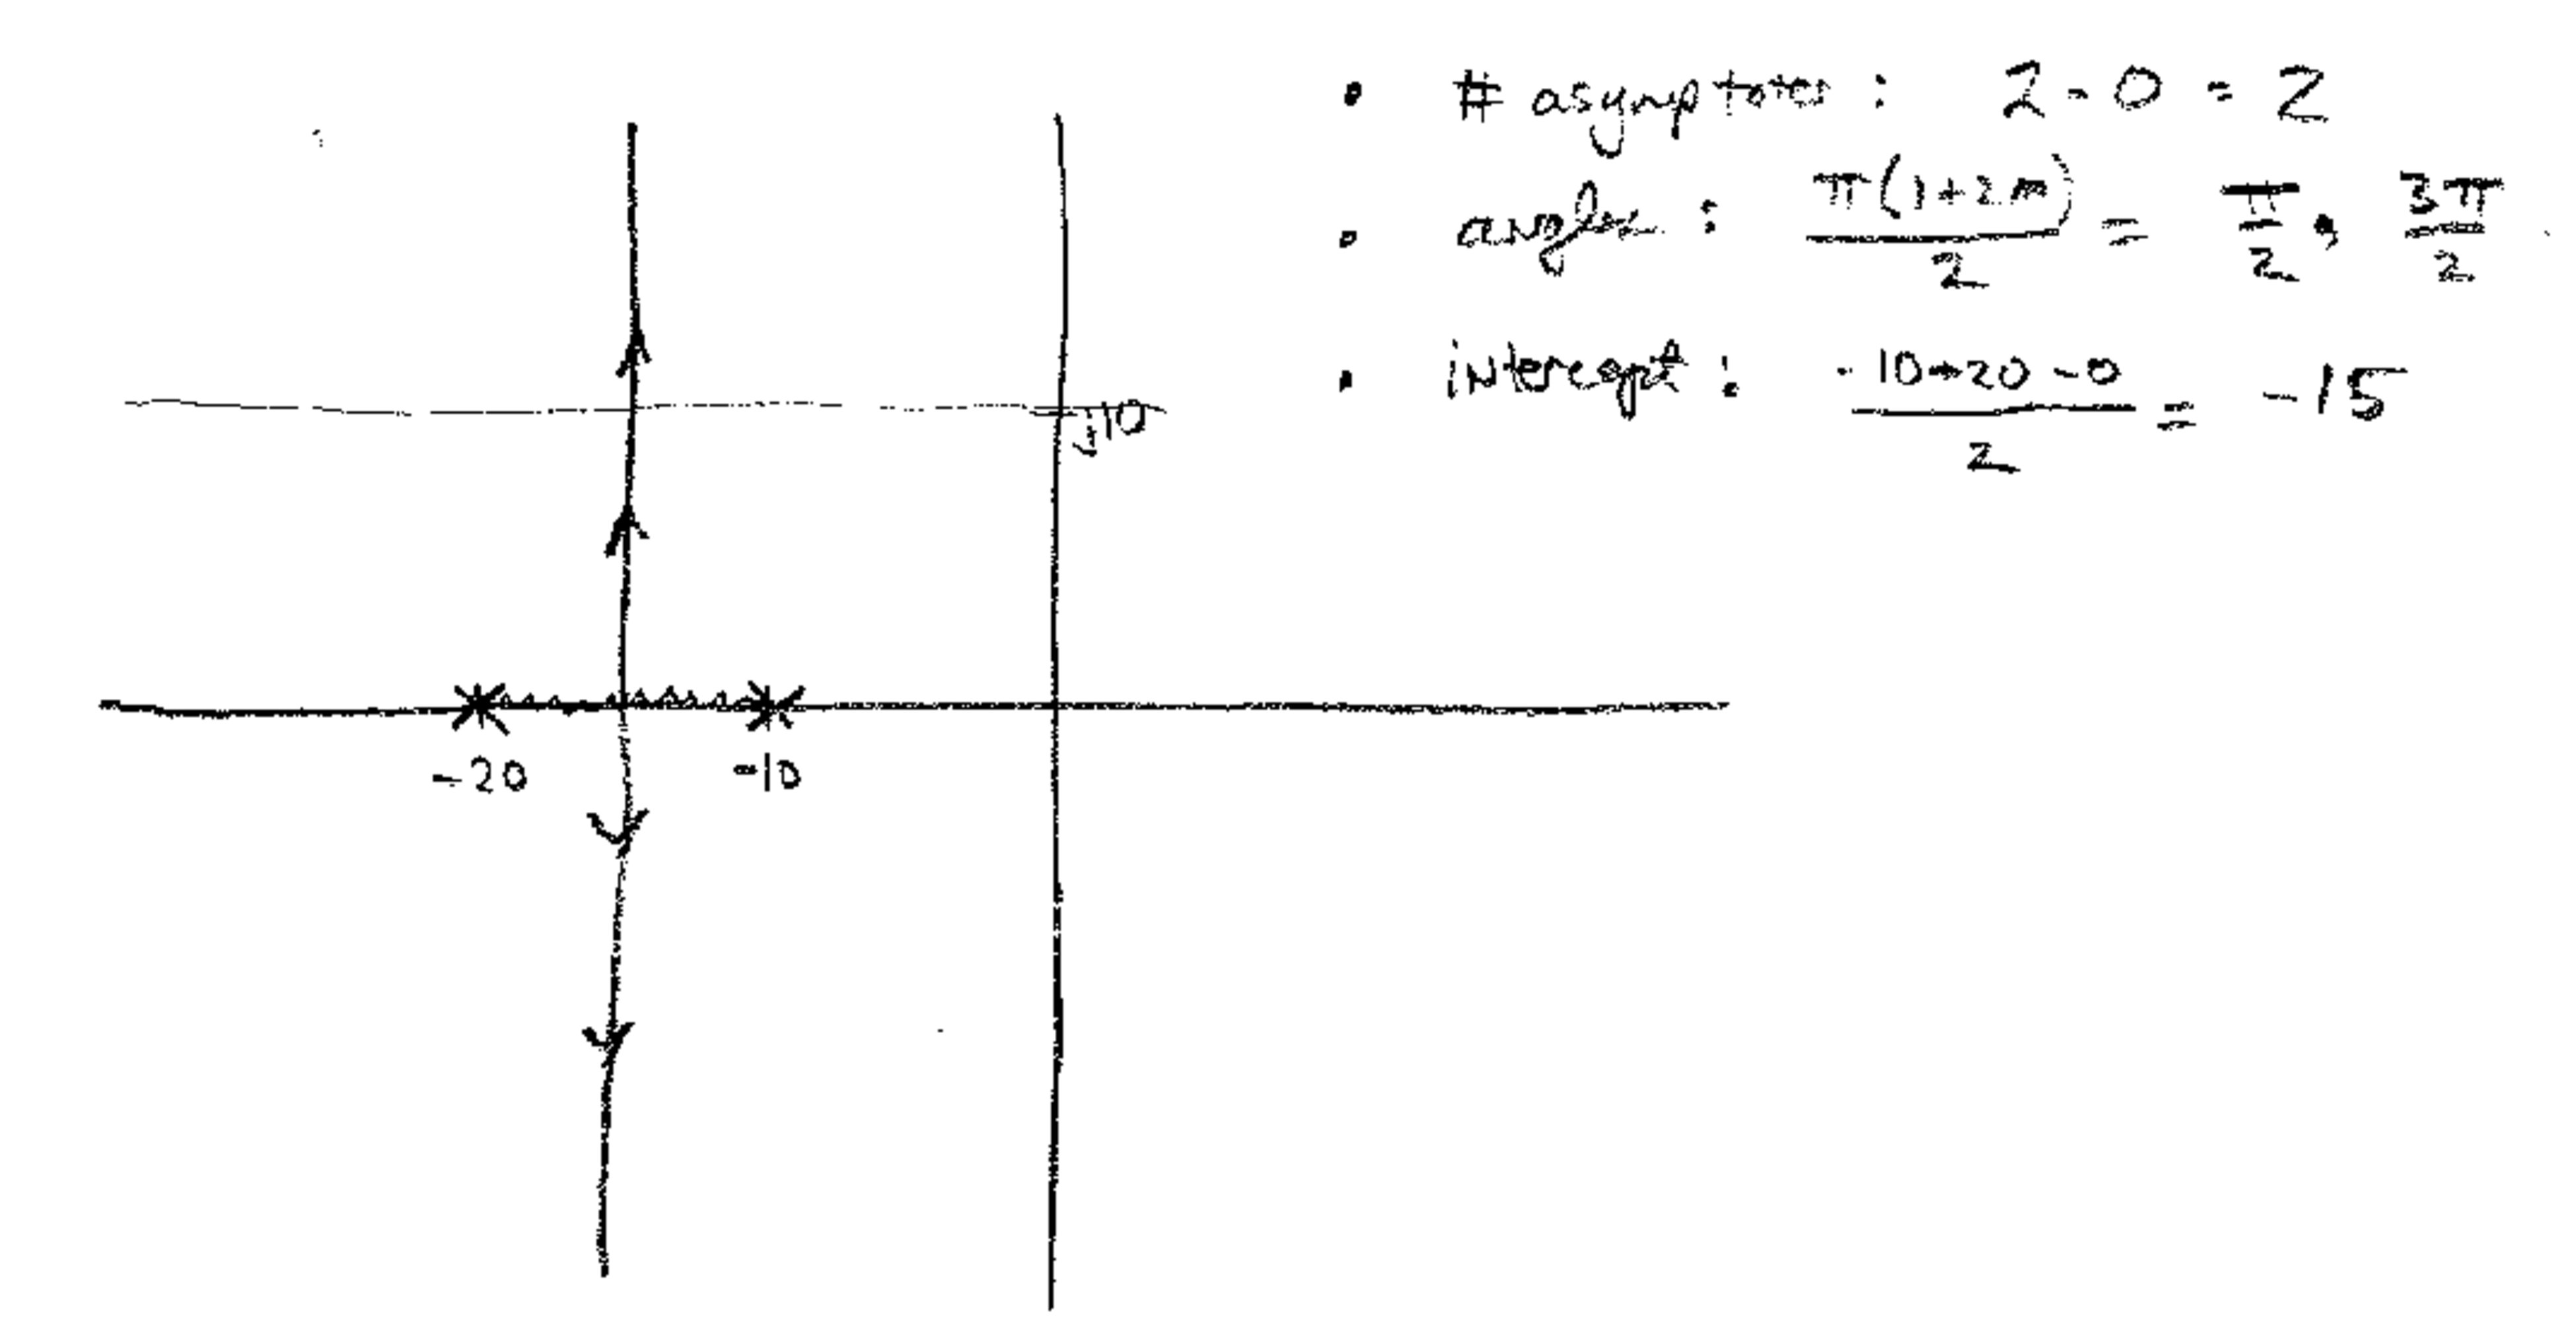
\includegraphics[width=13cm]{00551a.png}	%<n>


	%<*>



%%%%%%%%%%%%%%%%%%%%%%%%%%%%%%%%%%%%%%%%%%%%%%%%%%%%%%%%%%%%%%%%%%%%%%%%%%%%%%%%%%%%%%%%%%%%%%%%
%%%%** Section 6.1.2 
\subsubsection{}  Find the value of $K$ at the point where the RL intersects the line $y=j10$.  Hint: use the magnitude condition.

 {\tt SOLUTION: }	%<*n>

From \ref{xx1}, the RL intersection point is $s=-15+j10$.

By the magnitude condition:
\[
K\times \left | \frac{1}{(s+10)(s+20)} \right | = 1
\]
\[
K = |(-15+j10+10)(-15+j20+20)| = |(-5+j10)||(5+j10|
\]
\[
K = (\sqrt{5^2+10^2} )^2 = 125
\]
	%<*>



	%<*>
%%%%%%%%%%%%%%%%%%%%%%%%%%%%%%%%%%%%%%%%%%%%%%%%%%%%%%%%%%%%%%%%%%%%%%%%%%%%%%%%%%%%%%%%%%%%%%%%
%%%%** Section 6.2
\subsection{}  Plot the Root Locus of
\[
CPH(s) = \frac{K(s+1)}{(s+5+j)(s+5-j)}
\]

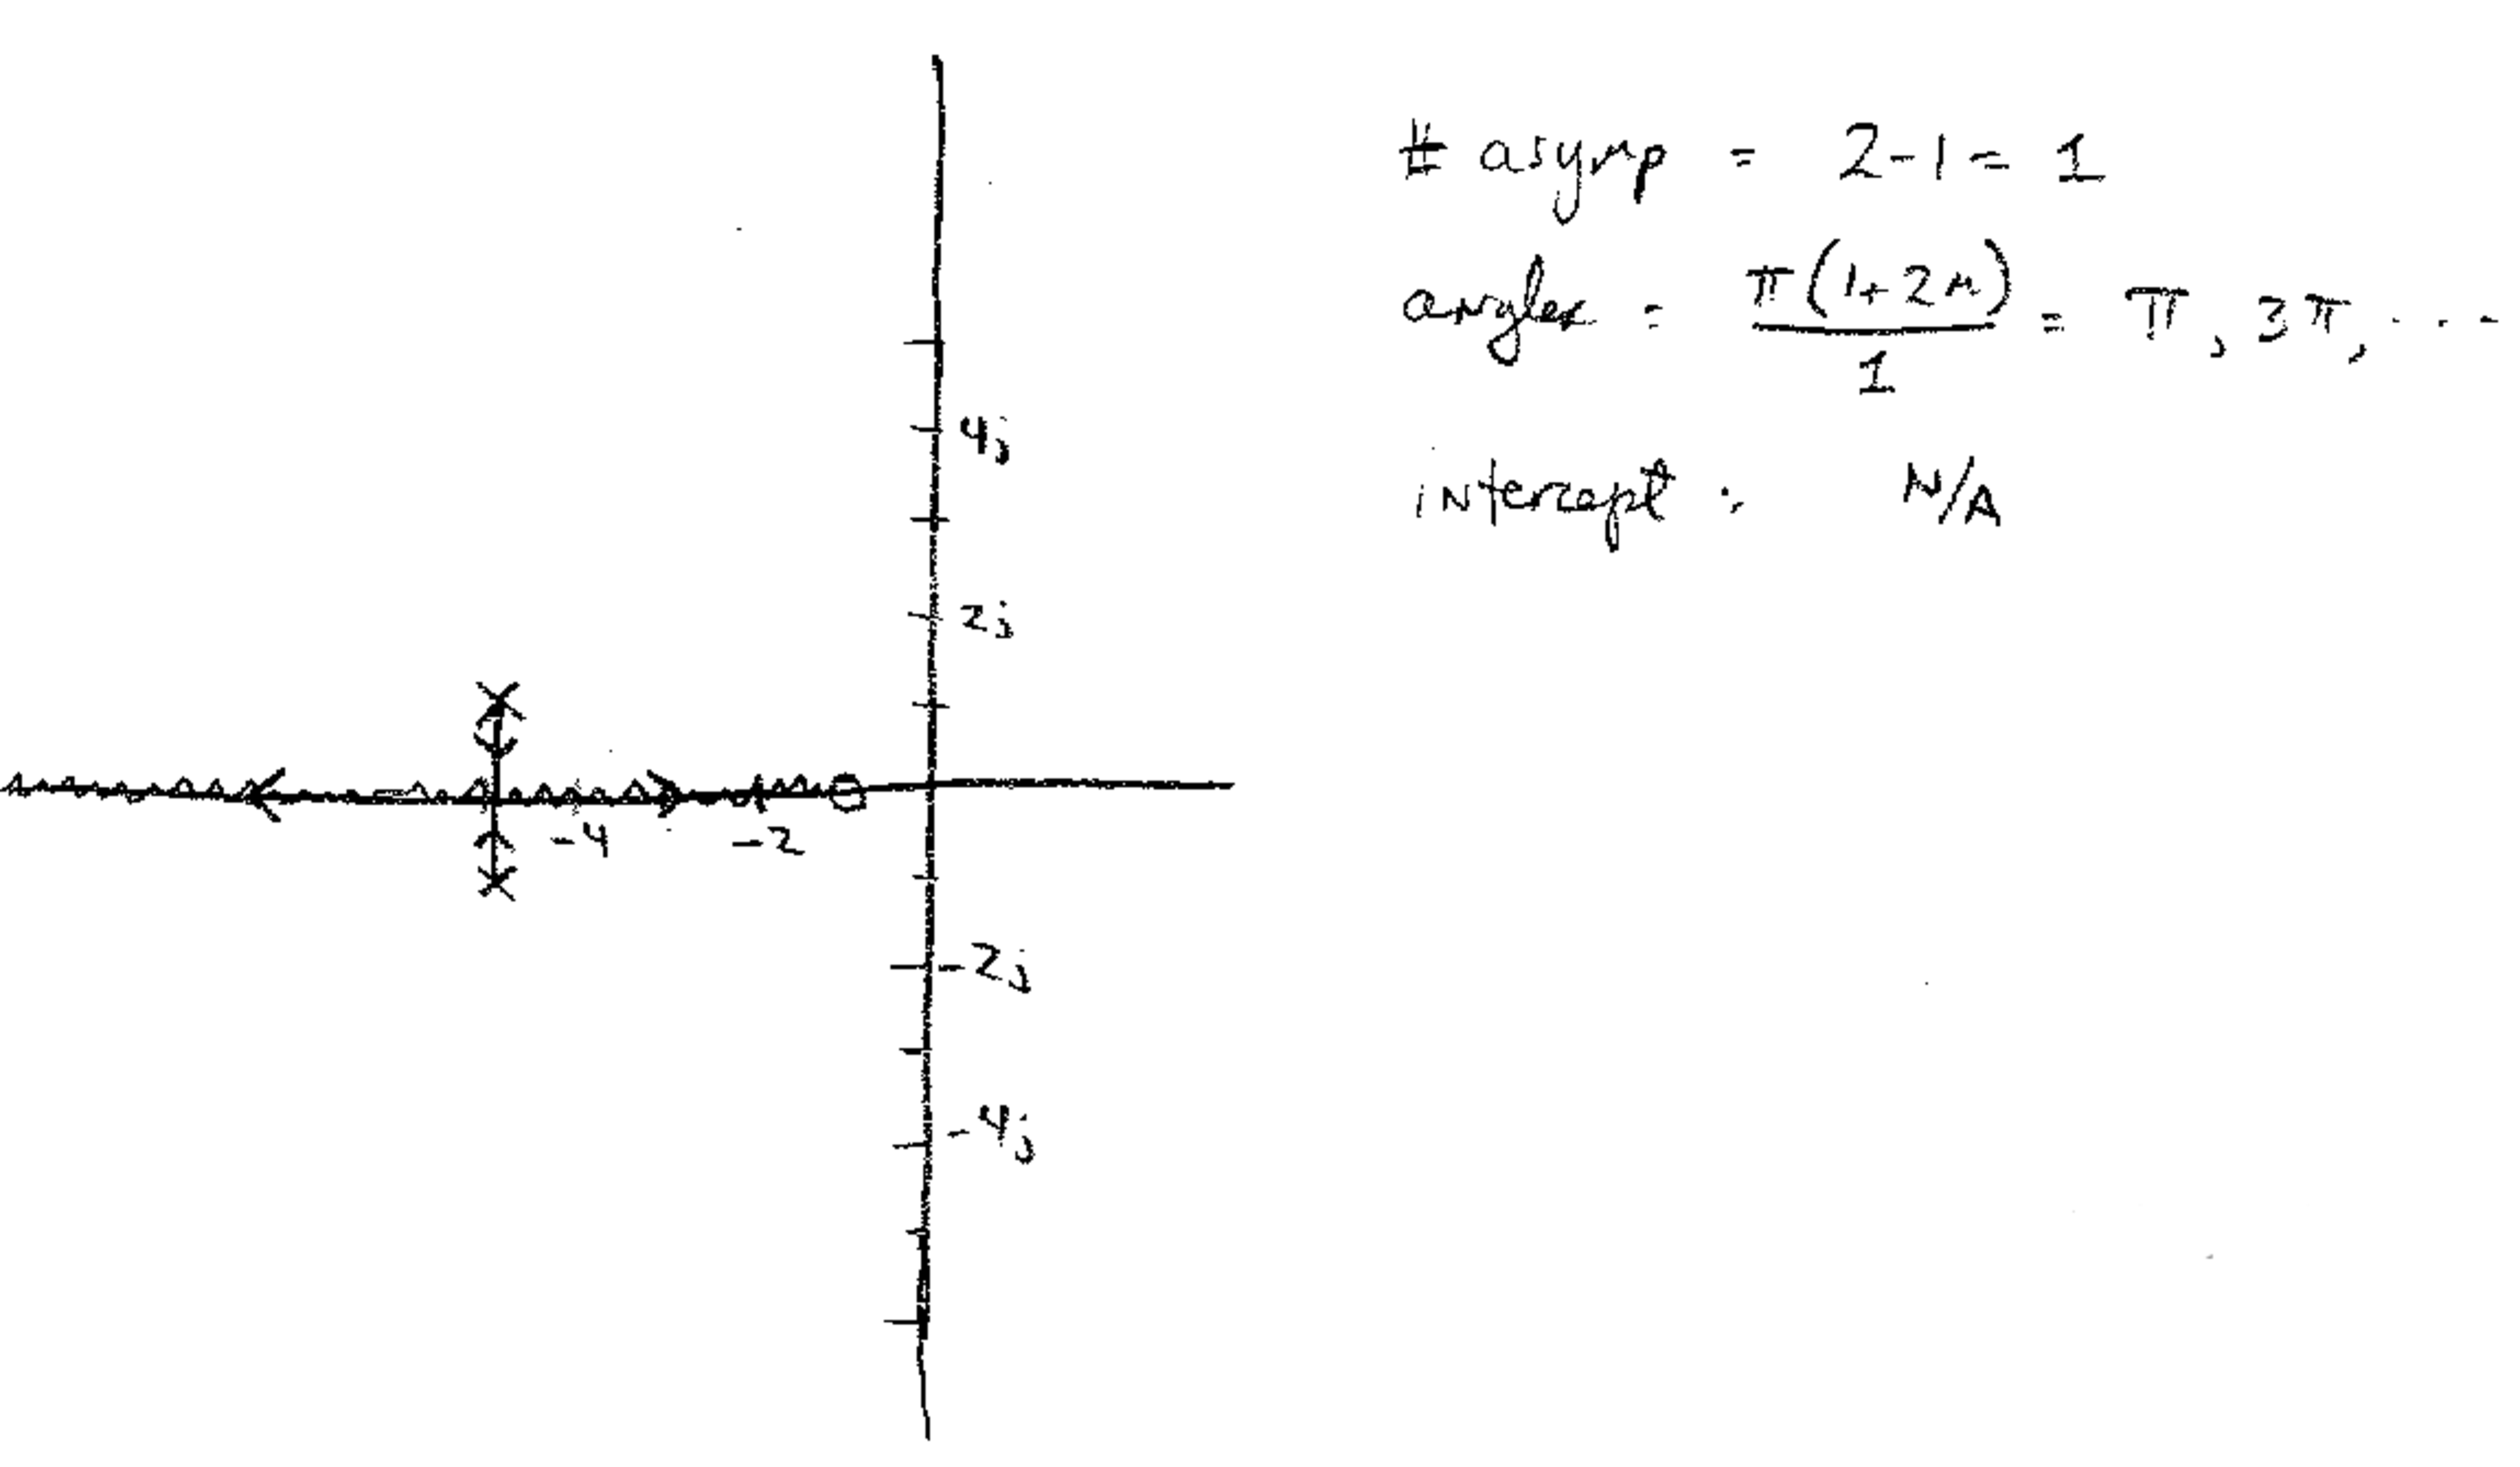
\includegraphics[width=14cm]{00550a.png}	%<n>


	%<*>
%%%%%%%%%%%%%%%%%%%%%%%%%%%%%%%%%%%%%%%%%%%%%%%%%%%%%%%%%%%%%%%%%%%%%%%%%%%%%%%%%%%%%%%%%%%%%%%%
%%%%** Section 6.3
\subsection{}  Plot the Root Locus of
\[
CPH(s) = \frac{K(s+6)}{s(s+3+j3)(s+3-j3)}
\]

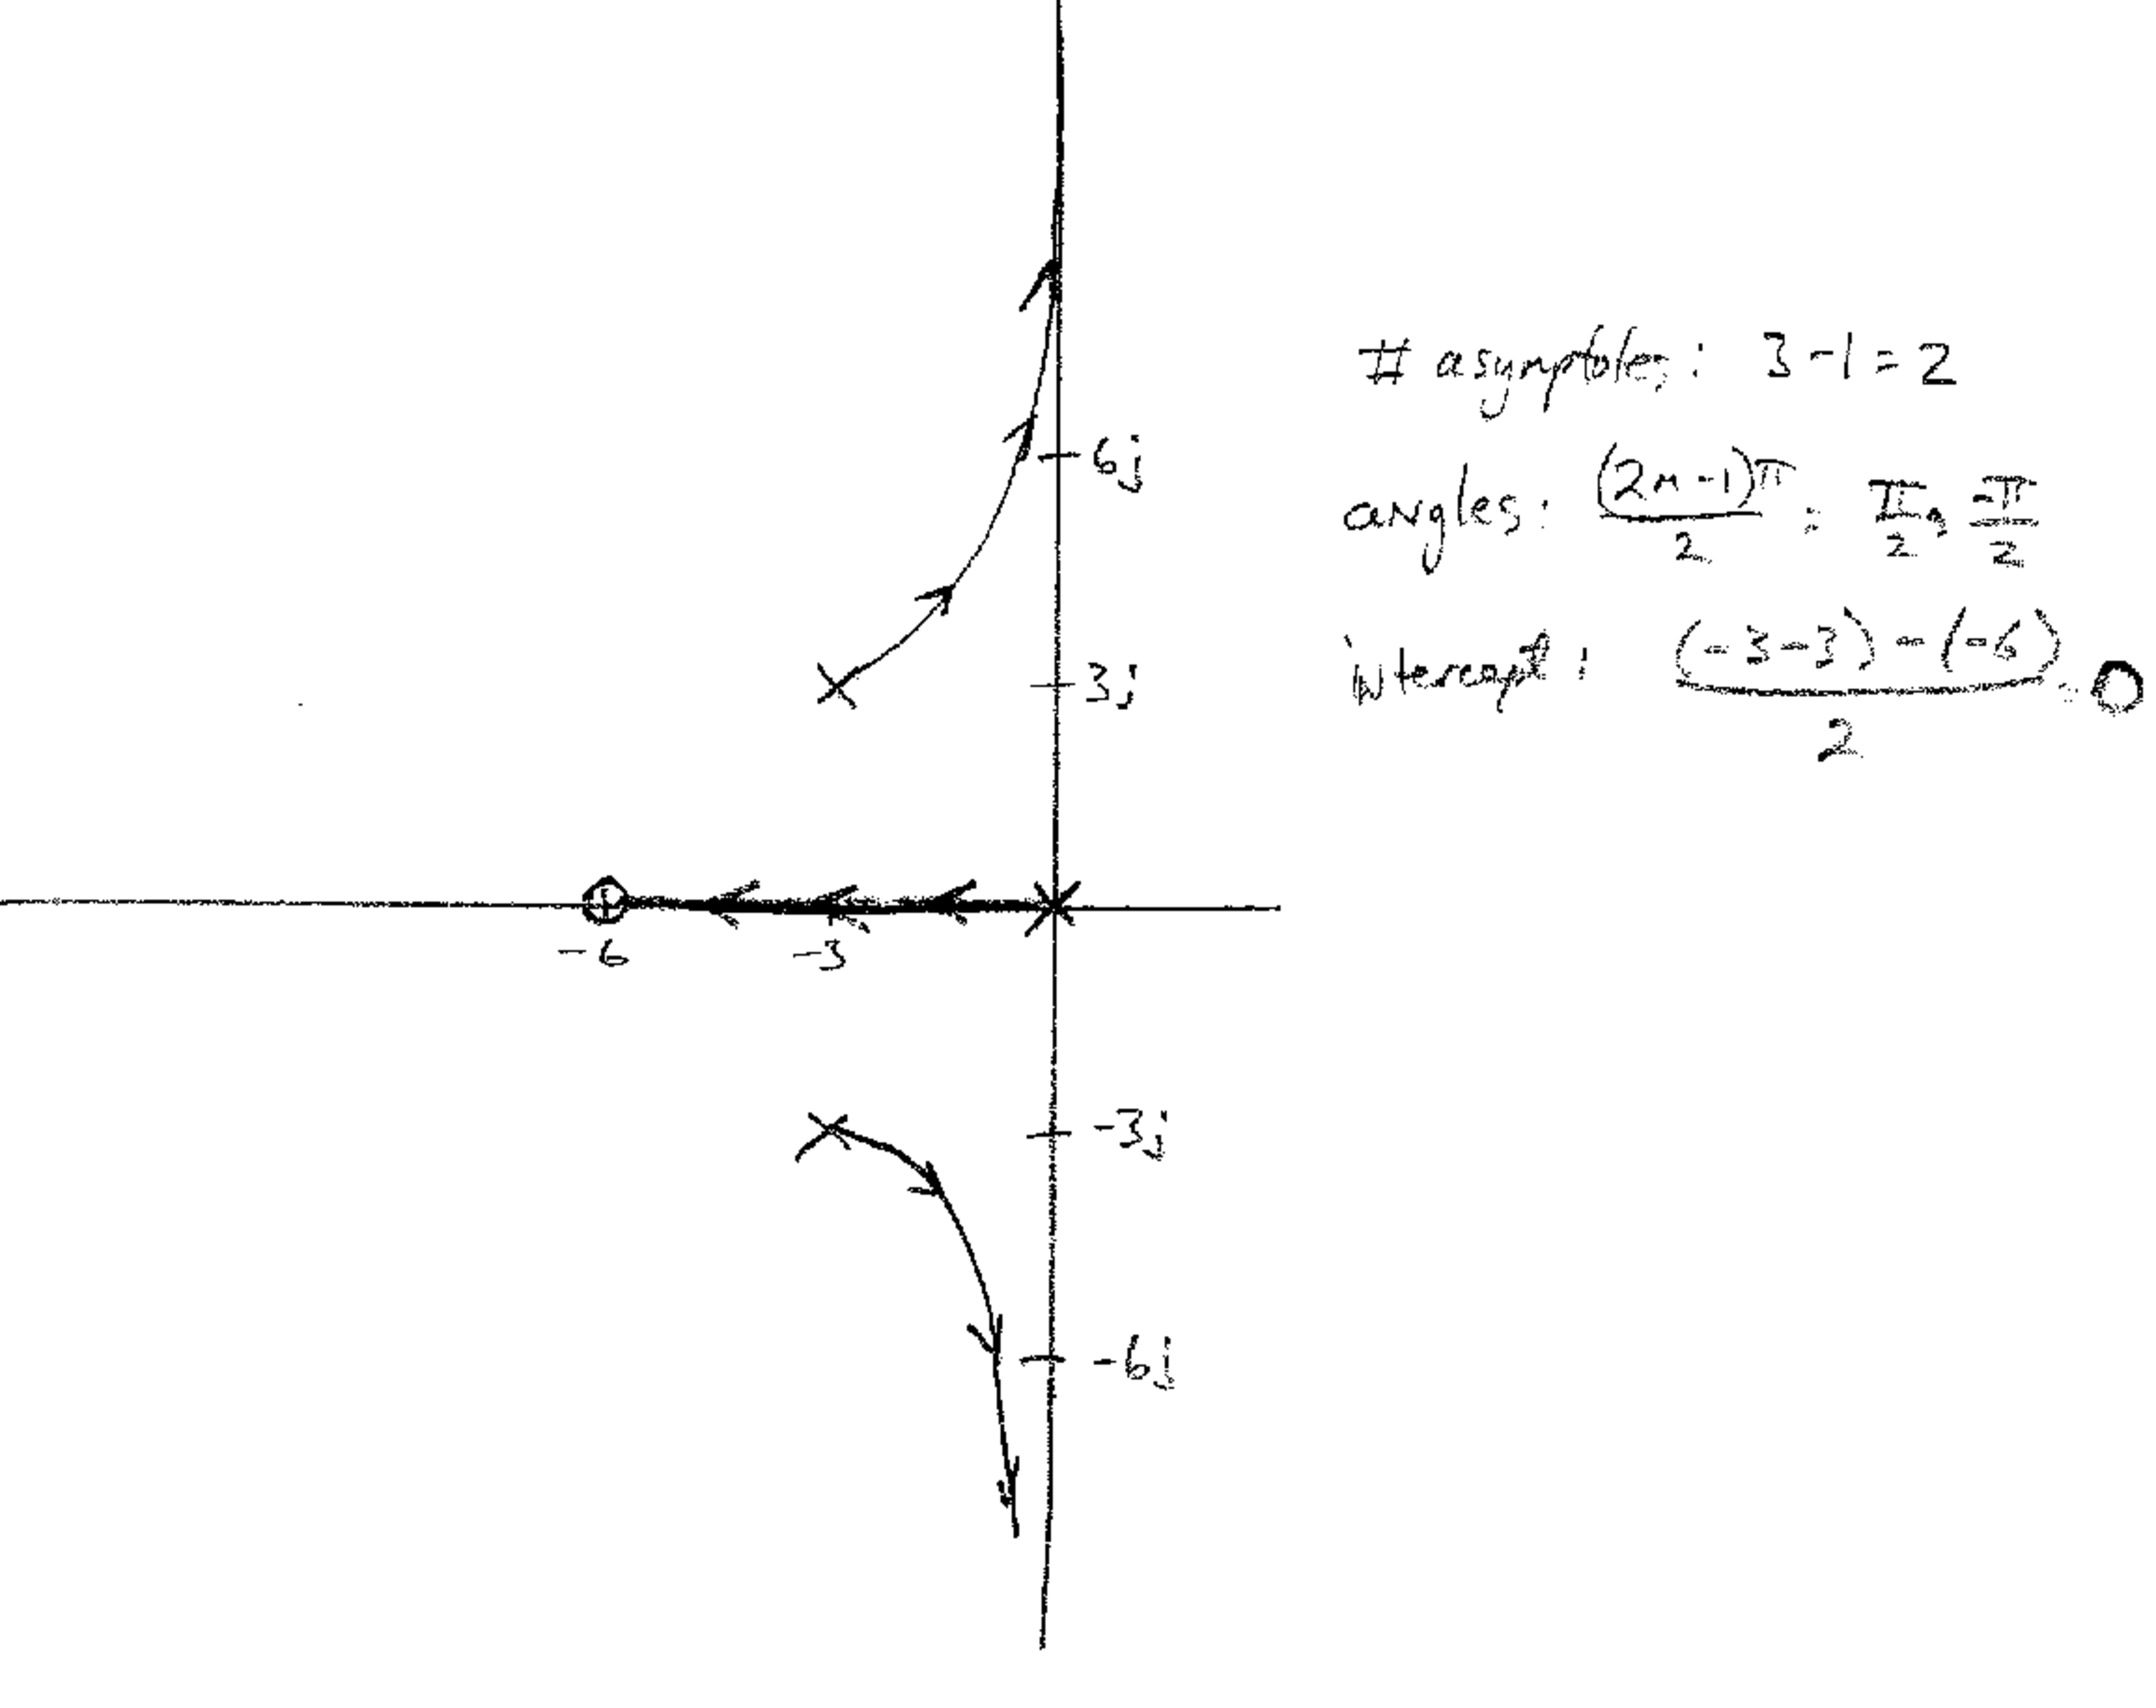
\includegraphics[width=14cm]{00558a.png}	%<n>

	%<*>
%%%%%%%%%%%%%%%%%%%%%%%%%%%%%%%%%%%%%%%%%%%%%%%%%%%%%%%%%%%%%%%%%%%%%%%%%%%%%%%%%%%%%%%%%%%%%%%%%%
%%%%** Section 6.4
\subsection{}

Plot the root locus for
\[
CPH(s) = \frac{K(s^2+6s+73)}{s(s+4)(s+4+4j)(s+4-4j)} \qquad K>0
\]


	%<*n>
\begin{solution}
Here's a valid hand drawn solution:

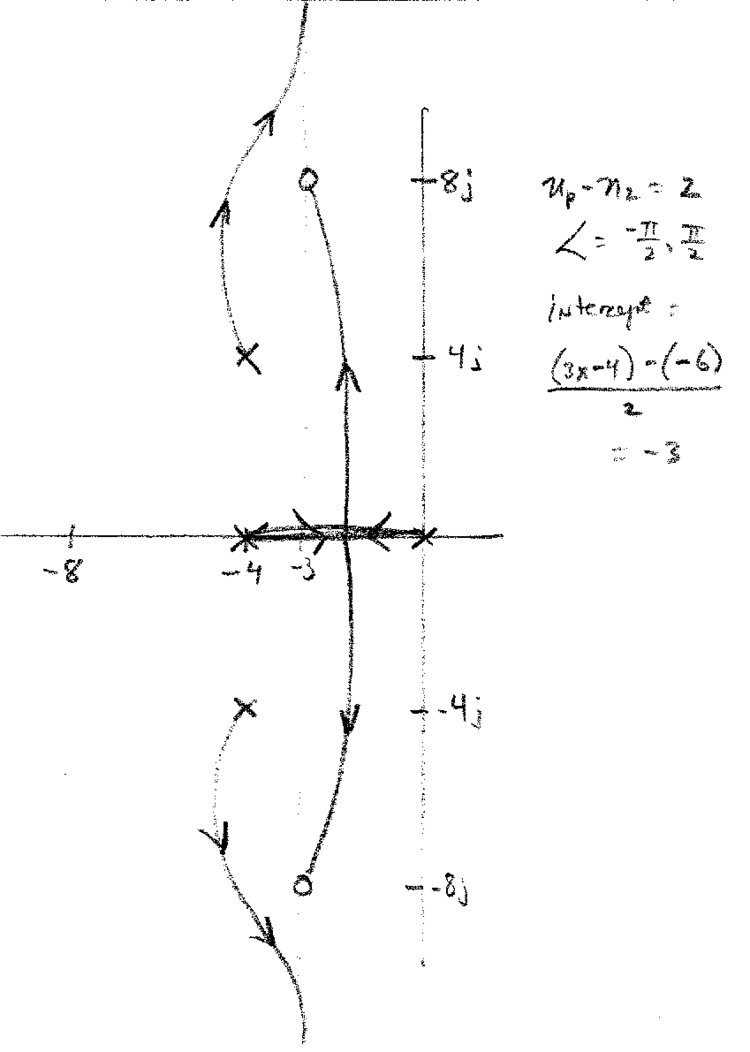
\includegraphics[width=2.5in]{00569a.png}


The computer solution:

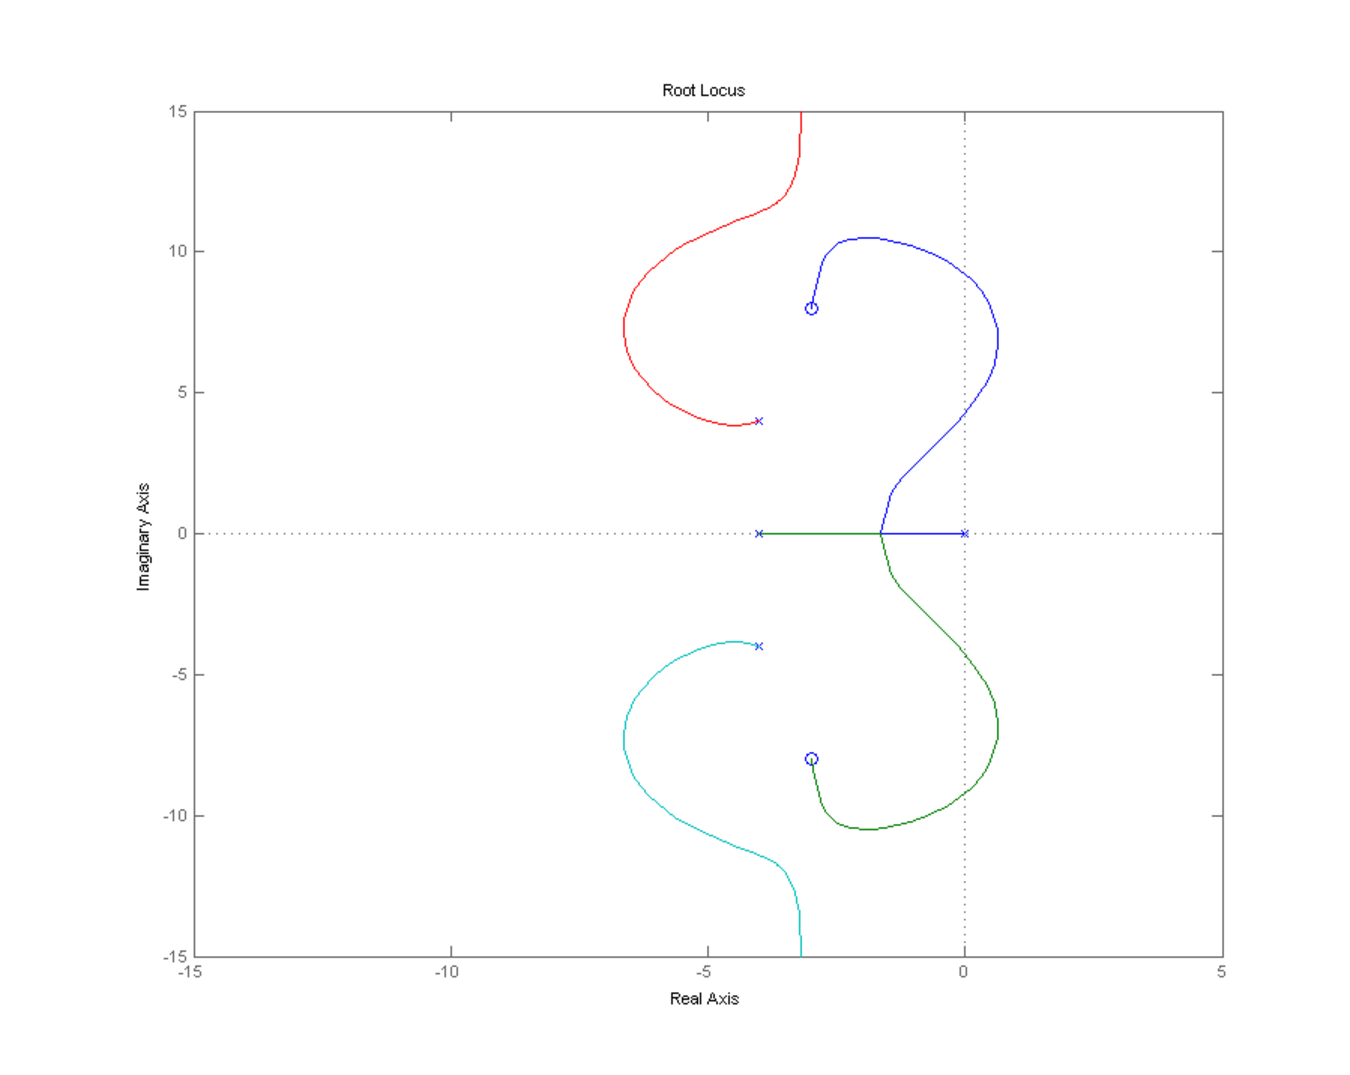
\includegraphics[width=4.5in]{mt2_rla.png}

Seems quite different!   If you look though, it agrees with everything in our calculation method.   If we had done the departure angles by hand (the old way) we would have drawn something close to this!
\end{solution}
	%<*>




%%%%%%%%%%%%%%%%%%%%%%%%%%%%%%%%%%%%%%%%%%%%%%%%%%%%%%%%%%%%%%%%%%%%%%%%%%%%%%%%%%%%%%%%%%%%%%%%
%%%%** Section 6.5
\subsection{}\label{basicRL}

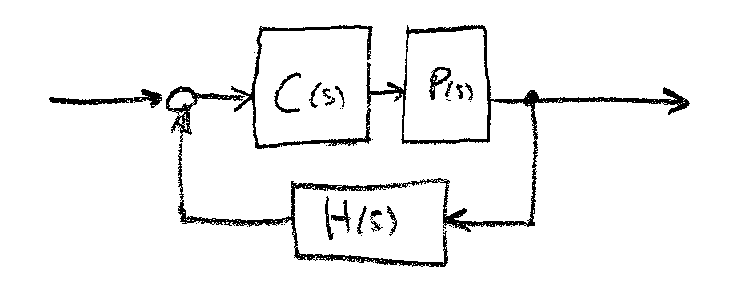
\includegraphics[width=3.5in]{00479.png}

For $C(s) = C_1(s) = \frac{K}{(s+10)}$ and $P(s) = \frac{4}{(s+0.5-2j)(s+0.5+2j)}$, $H(s) = 1$, plot the
root locus by hand for $K\geq 0$.

	%<*n>
\begin{solution}
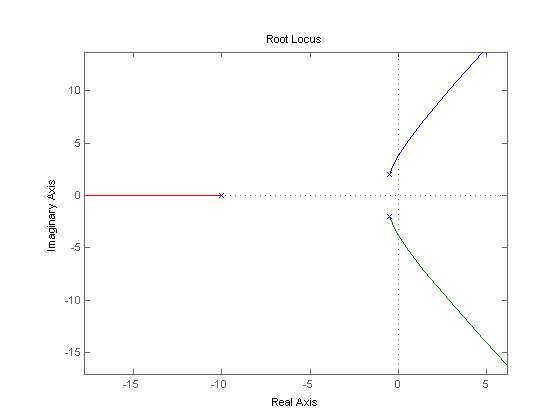
\includegraphics[width=4.5in]{hw7_6.png}
\end{solution}
	%<*>




%%%%%%%%%%%%%%%%%%%%%%%%%%%%%%%%%%%%%%%%%%%%%%%%%%%%%%%%%%%%%%%%%%%%%%%%%%%%%%%%%%%%%%%%%%%%%%%%%%%%%%%%%%%%%%%%%%%%%%%%%%%%%%%%%%%%

%%%%** Section 6.6
\subsection{}
Redo the root locus of Problem \ref{basicRL} for $C(s) = C_2(s) = \frac{K(s+4)}{(s+10)}$, $P, H$ unchanged.

Comment on the stability of the closed loop system with this controller compared to $C_1(s)$ of Problem \ref{basicRL}.


	%<*n>
\begin{solution}
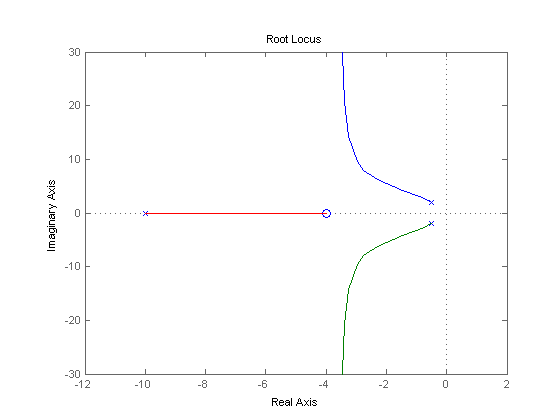
\includegraphics[width=4.5in]{hw7_7.png}

Addition of a zero in the controller has made the system more stable by moving the RL to the left.
\end{solution}


	%<*>






%%%%%%%%%%%%%%%%%%%%%%%%%%%%%%%%%%%%%%%%%%%%%%%%%%%%%%%%%%%%%%%%%%%%%%%%%%%%%%%%%%%%%%%%%%%%%%%%%%
%%%%** Section 6.7
\subsection{}
Plot the Root Locus for
\[
G(s) = \frac {K(s+3)(s+1)}
{(s+2)(s^2+6s+10)(s+1+j)(s+1-j)}  \qquad  K>0
\]



Be sure to give your calculations for number of asymptotes, intercept of asymptotes, angle of asymptotes, etc.

	%<*n>
\begin{solution}

\[
n_p-n_z = 3 \qquad \angle = \pi/3, \pi, -\pi/3
\]

Intercept = $\frac{-2+2\times(-3)+2\times(-1) - (-1-3)}{3} = \frac{-6}{3} = -2$

Real Line occupied by RL:   $-2 < \sigma < -1, \quad \sigma < -3$.

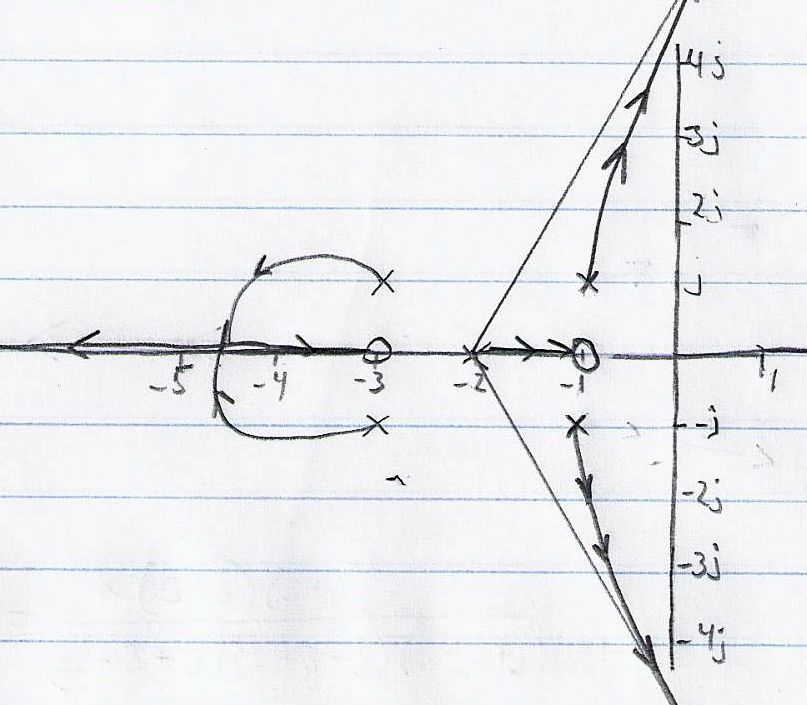
\includegraphics[width=125mm]{rl.png}


\end{solution}

	%<*>






%%%%%%%%%%%%%%%%%%%%%%%%%%%%%%%%%%%%%%%%%%%%%%%%%%%%%%%%%%%%%%%%%%%%%%%%%%%%%%%%%%%%%%%%%%%%%%%%%%%%%
%%%%%%%%%%%%%%%%%%%%%%%%%%%%%%%%%%%%%%%%%%%%%%%%%%%%%%%%%%%%%%%%%%%%%%%%%%%%%%%%%%%%%%%%%%%%%%%%%%%%%
\newpage
%%%%** Section 7 
\section{EE447 In Class Problems: SSE and Closed Loop Performance}

In this ICP set there is a mix of hand and computer problems.  Please bring a laptop to class.  If you do not have a laptop, share with a friend!   (In many classrooms there are very few power outlets so charge it up first!).

To receive credit for your hand work, turn in paper as usual.  For your computer work there are multiple options, but only one will be used.   We will announce which method will be used in class:

\begin{enumerate}
  \item Show your work to the professor or a TA and they will note completion and initial on your hard copy.
  \item Copy your graphic output and computer scripts into a word doc.  Export to PDF.  Upload into the \href{https://canvas.uw.edu/courses/1116153/assignments/3823644}{"ICP 7" assignment in Canvas/Gradescope}.
\end{enumerate}

You may use Matlab if you prefer.   However, ICP 8 will {\bf require} Scilab use so this would be a good chance to get ready.


	%<*>
%%%%** Section 7.1
\subsection{Steady State Error (SSE)}
Find the system type for each of the systems below:

\renewcommand\arraystretch{2.0}% Vertical Row size, 1.0 is for standard spacing)
%
%\begin{tabular}{|l|c|}  \hline
%System							& Type \\ \hline
%$CPH(s) = \frac{250}        {s^2(s+0.1)(s+10)}$		&      \\ \hline
%$CPH(s) = \frac{20(s+0.2)}  {s(s+0.1)(s^2+10s)}$	&      \\ \hline
%$CPH(s) = \frac{5\times10^4}{(s^3+10s^2+126s+3000)}$	&      \\ \hline
%$CPH(s) = \frac{20(s+2)}    {s(s+0.2)}$			&      \\ \hline
%$CPH(s) = \frac{100(s+0.01)}{s^4+5s^3+50s^2}$		&      \\ \hline
%\end{tabular}
	%<*n>
\begin{tabular}{|l|c|}  \hline
System							& Type \\ \hline
$CPH(s) = \frac{250}        {s^2(s+0.1)(s+10)}$		&  2   \\ \hline
$CPH(s) = \frac{20(s+0.2)}  {s(s+0.1)(s^2+10s)}$	&  2   \\ \hline
$CPH(s) = \frac{5\times10^4}{(s^3+10s^2+126s+3000)}$	&  0   \\ \hline
$CPH(s) = \frac{20(s+2)}    {s(s+0.2)}$			&  1   \\ \hline
$CPH(s) = \frac{100(s+0.01)}{s^4+5s^3+50s^2}$		&  2   \\ \hline
\end{tabular}

	%<*>

%\end{frame}  %%%%%%%%%%%%%%%%%%%%%%%%%%%%%%%%%%%%%%%%%%%%%%%%%%%%%%%%%%%%



%\begin{frame}


	%<*>
%%%%** Section 7.2
\subsection{} Let $C(s) = 50$, $P(s) = \frac{200(s+1)}{s(s+3)(s+50)}$, $H(s)  = 1$.


	%<*>
%%%%** Section 7.2.1 
\subsubsection{} What is the system type?

 {\bf SOLUTION: }	%<*n>
 1, there is one power of $s$ at the origin.

	%<*>

	%<*>
%%%%** Section 7.2.2 
\subsubsection{}  If $x(t) = 0.2t^2$, what is  the SSE?

 {\bf SOLUTION: }    The system type is 1.  The input is parabolic.  Thus the SSE is $\infty$.	%<n>


	%<*>
%%%%** Section 7.2.3 
\subsubsection{} What is the SSE of this system for $x(t) = 100u(t)$?

 {\bf SOLUTION: }    The system type is 1.  The input is a step.  Thus the SSE must be $0$.	%<n>


	%<*>
%%%%** Section 7.2.4 
\subsubsection{} What is the SSE of this system for $x(t) = 0.01t$?

 {\bf SOLUTION: }    The system type is 1.  The input is a ramp.  Thus the SSE must be finite.  Specifically,	%<*n>

\[
X(s) = 0.01/s^2
\]
\[
E(s) = \frac{X(s)}{1+CPH} = \frac{0.01/s^2}{1+\frac{50\times200(s+1)}{s(s+3)(s+50)}} =
\frac{\frac{0.01}{s^2}(s(s+3)(s+50))}
{s(s+3)(s+50)+10^4(s+1)}
\]
By the final value theorem:
\[
\mathrm{SSE} = \lim_{t\to\infty} e(t) = \lim_{s\to0} sE(s) =
\lim_{s\to0} \frac{s0.01s(s+3(s+50)}{s^2(s(s+3)(s+50)+1.0\times10^4(s+1))} =
\frac{0.01(3)(50)}{10^4} = 1.5\times10^{-4}
\]
	%<*>


%\end{frame}  %%%%%%%%%%%%%%%%%%%%%%%%%%%%%%%%%%%%%%%%%%%%%%%%%%%%%%%%%%%%



%%%%%%%%%%%%%%%%%%%%%%%%%%%%%%%%%%%%%%%%%%%%%%%%%%%%%%%%%%%%%%%%%%%%%%%%%%%%%%%%%%%%%%%%%%%%%%%%%%%%%%%%%
	%<*>
%%%%** Section 7.3
\subsection{}
  Which systems have zero steady state error for $x(t) = 10t$?\\[0.25in]

\begin{center}


% Make table rows deeper
\renewcommand\arraystretch{2.0}% Vertical Row size, 1.0 is for standard spacing)
\begin{tabular}{|l|l|}  \hline
A) $CPH(s) = \frac{K_A}{s(s+5)}$		&	B) $CPH(s) = \frac{K_B}{s^2(s+50)}$   \\  \hline
C) $CPH(s) = \frac{K_C}{s^3(s+100)}$		&	D) $CPH(s) = \frac{K_D}{s^2(s-10)}$   \\  \hline
\end{tabular}
\end{center}

	%<*n>
\begin{solution}
A) No, not high enough system 'type'

B) YES

C) YES

D) No - system has a positive pole and is thus unstable.
\end{solution}
	%<*>


	%<*>
%%%%** Section 7.4
\subsection{S-Plane Regions}

  Find the s-plane region for 2nd order poles corresponding to the following step response performance requirements;


	%<*>
%%%%** Section 7.4.1 
\subsubsection{}$1<T_s<3 \qquad 2\% < \%OS < 5\%$.

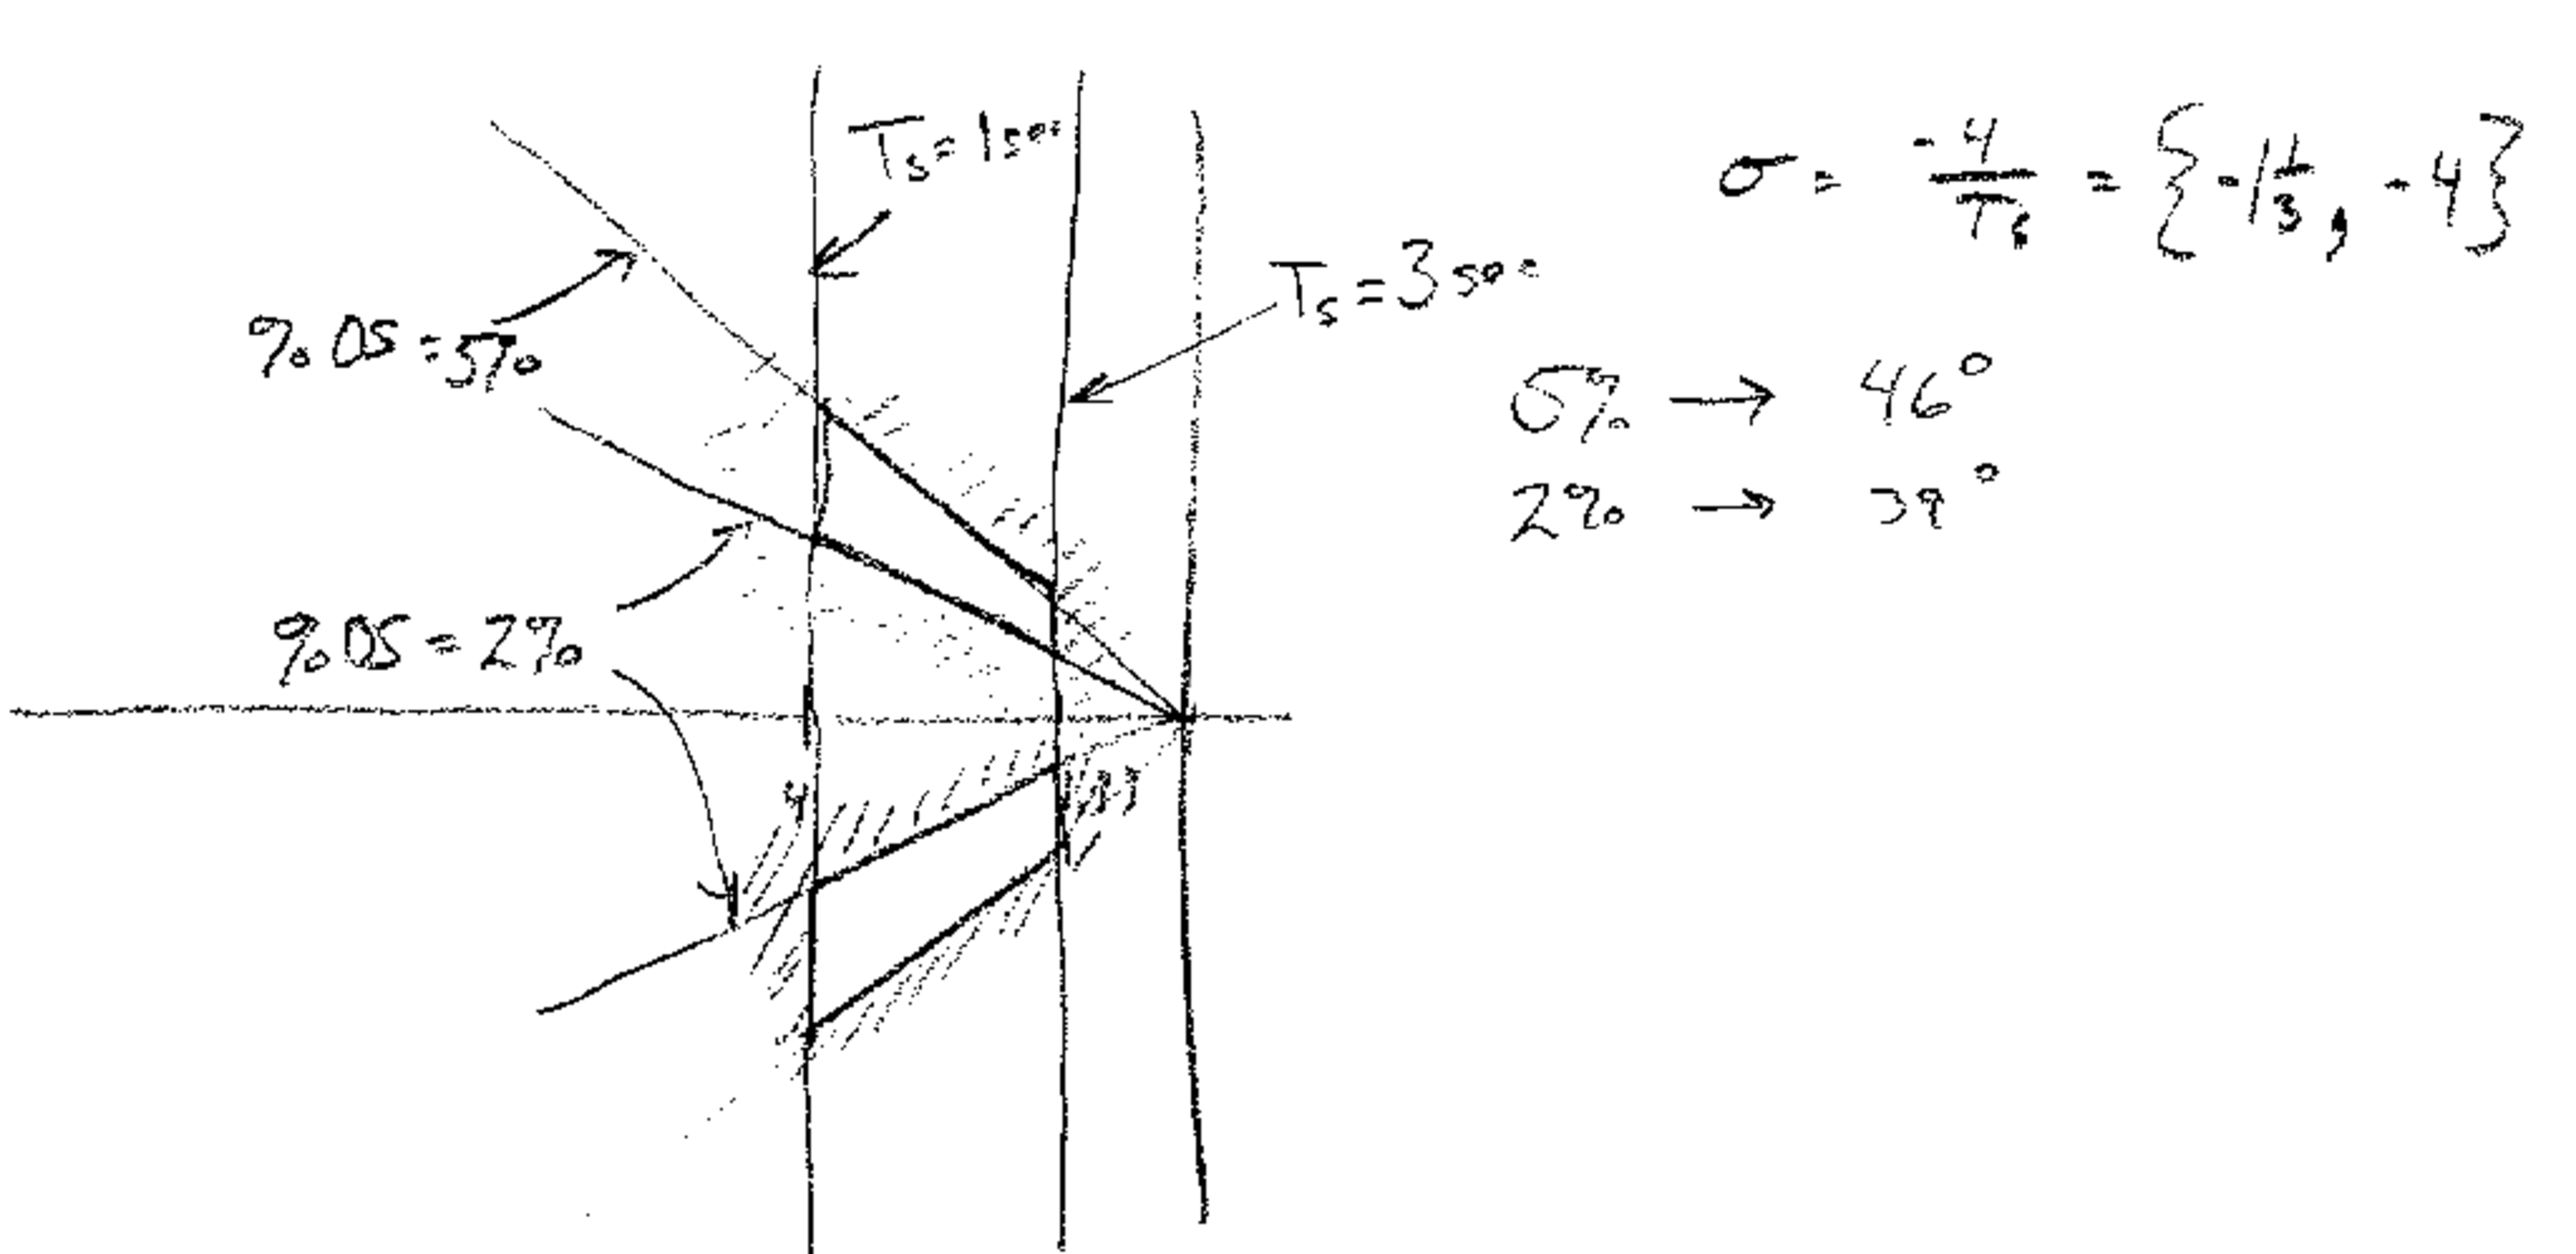
\includegraphics[width=12.5cm]{00547a.png}	%<n>


	%<*>
%%%%** Section 7.4.2 
\subsubsection{} $T_s = 2sec$, $\%OS = 2\%$.

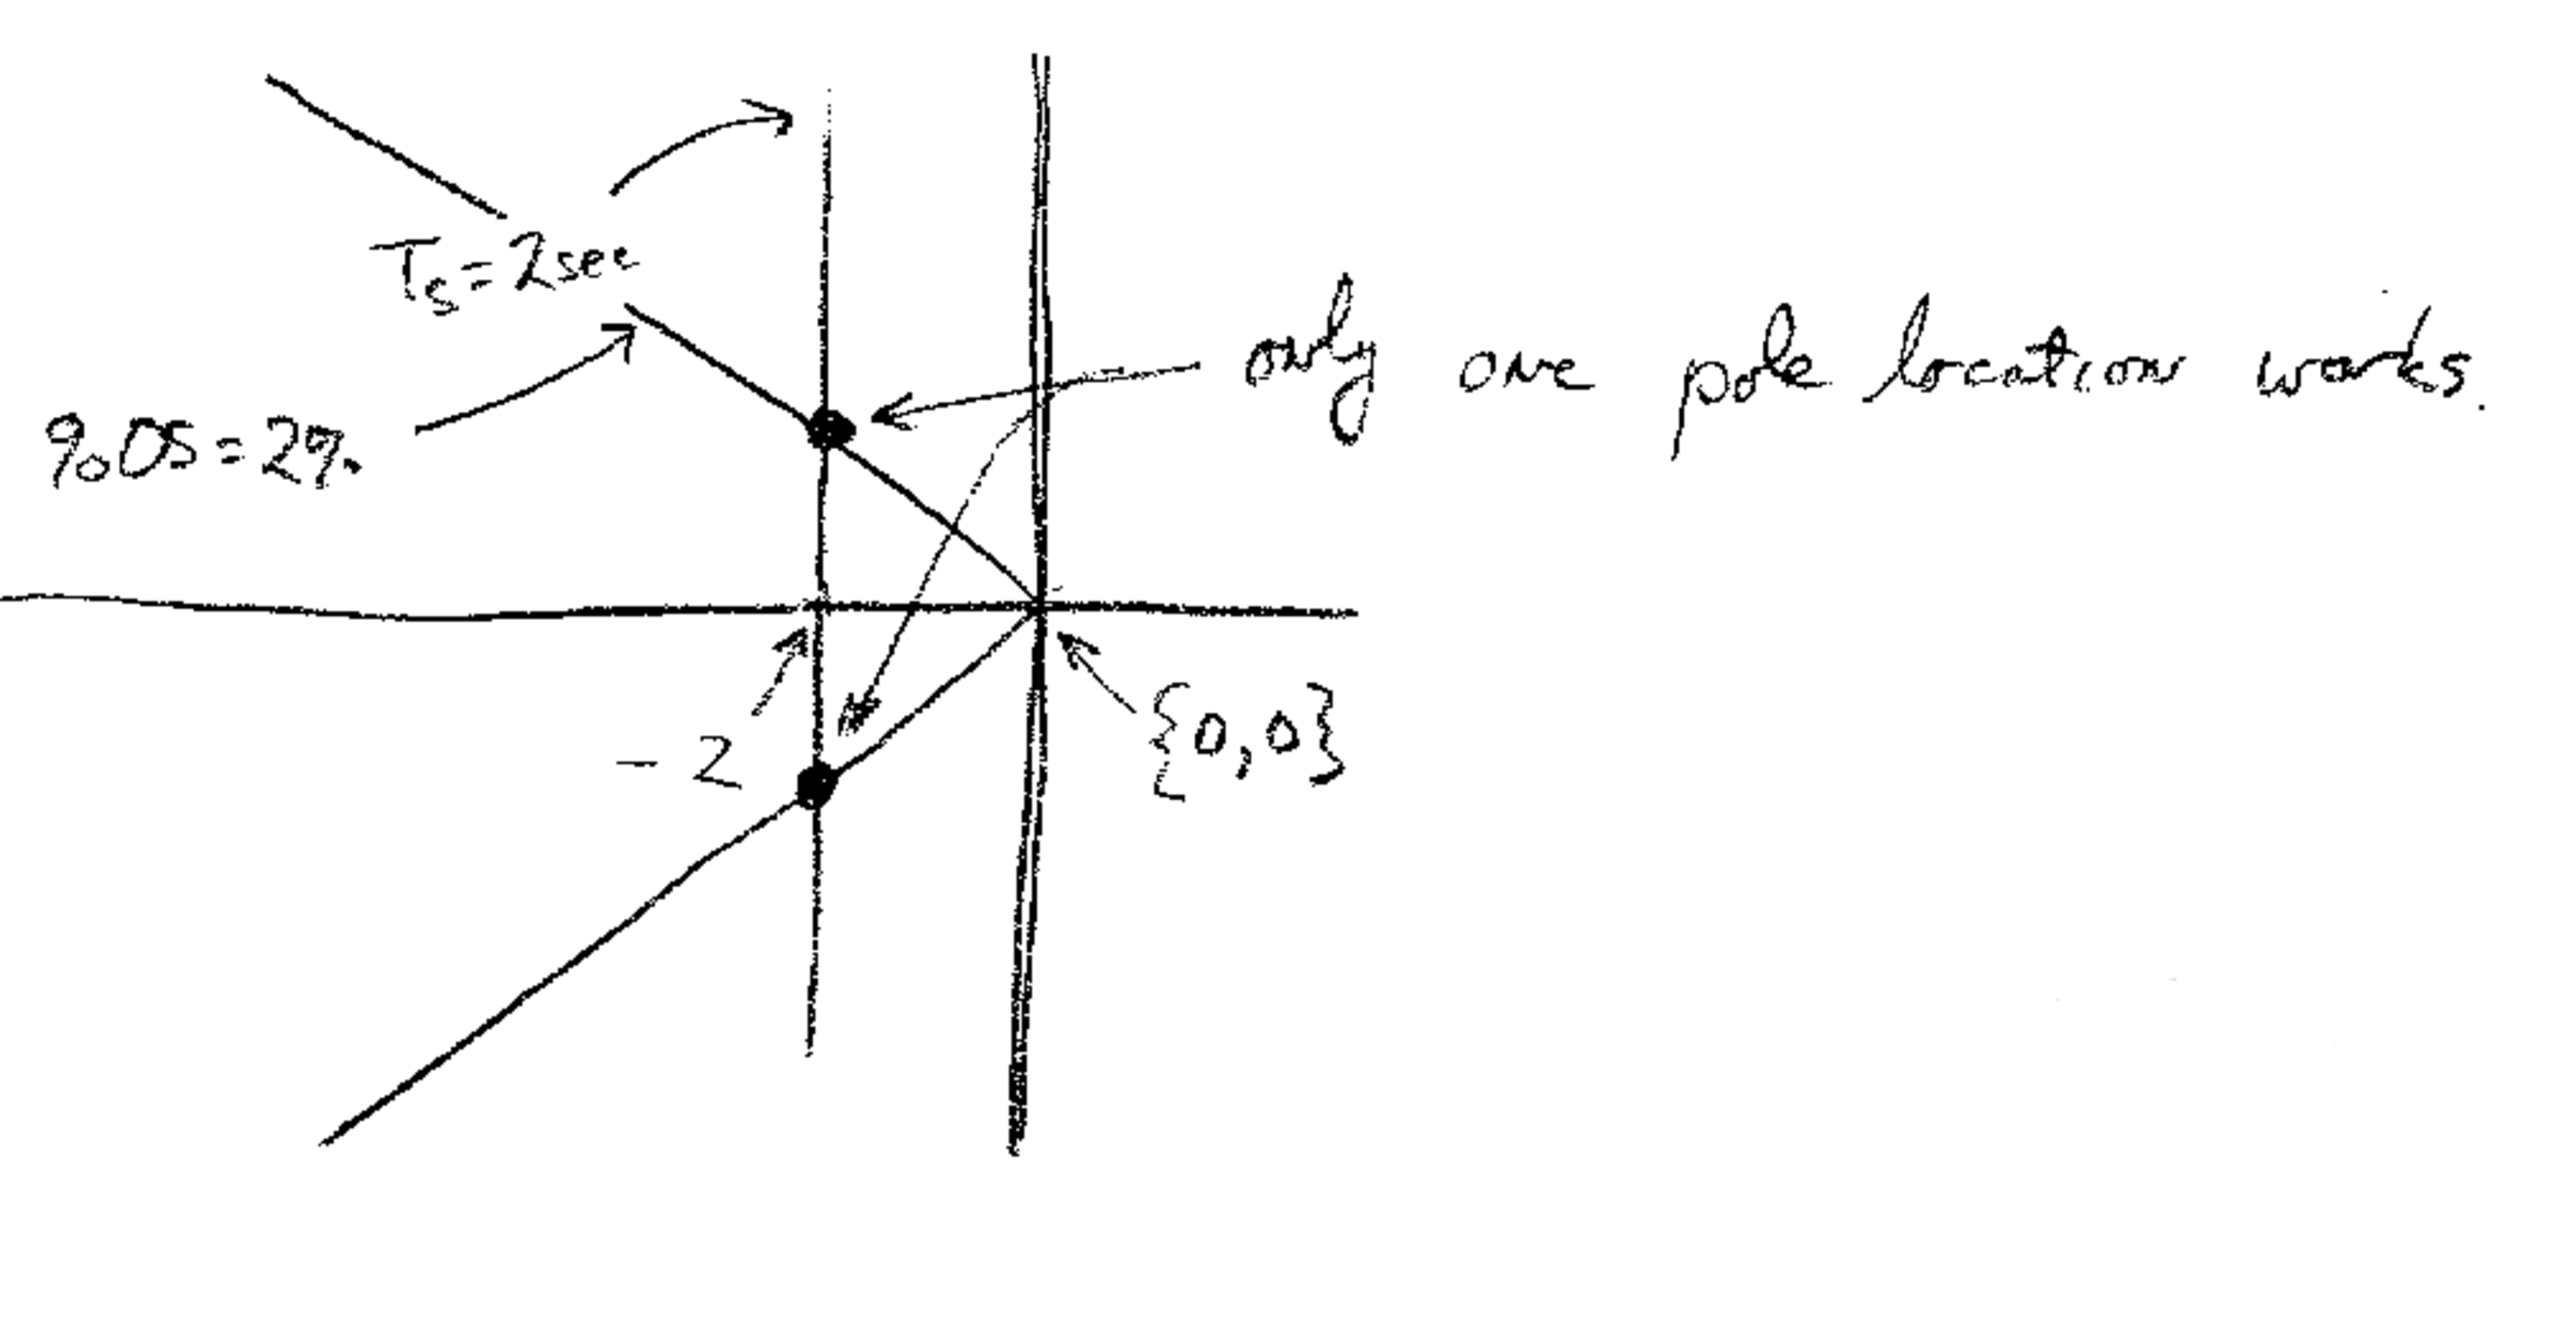
\includegraphics[width=12.5cm]{00548a.png}	%<n>



	%<*>
%%%%** Section 7.4.3 
\subsubsection{} $2<\omega_n<3.5$, $1sec < T_s < 2sec$.

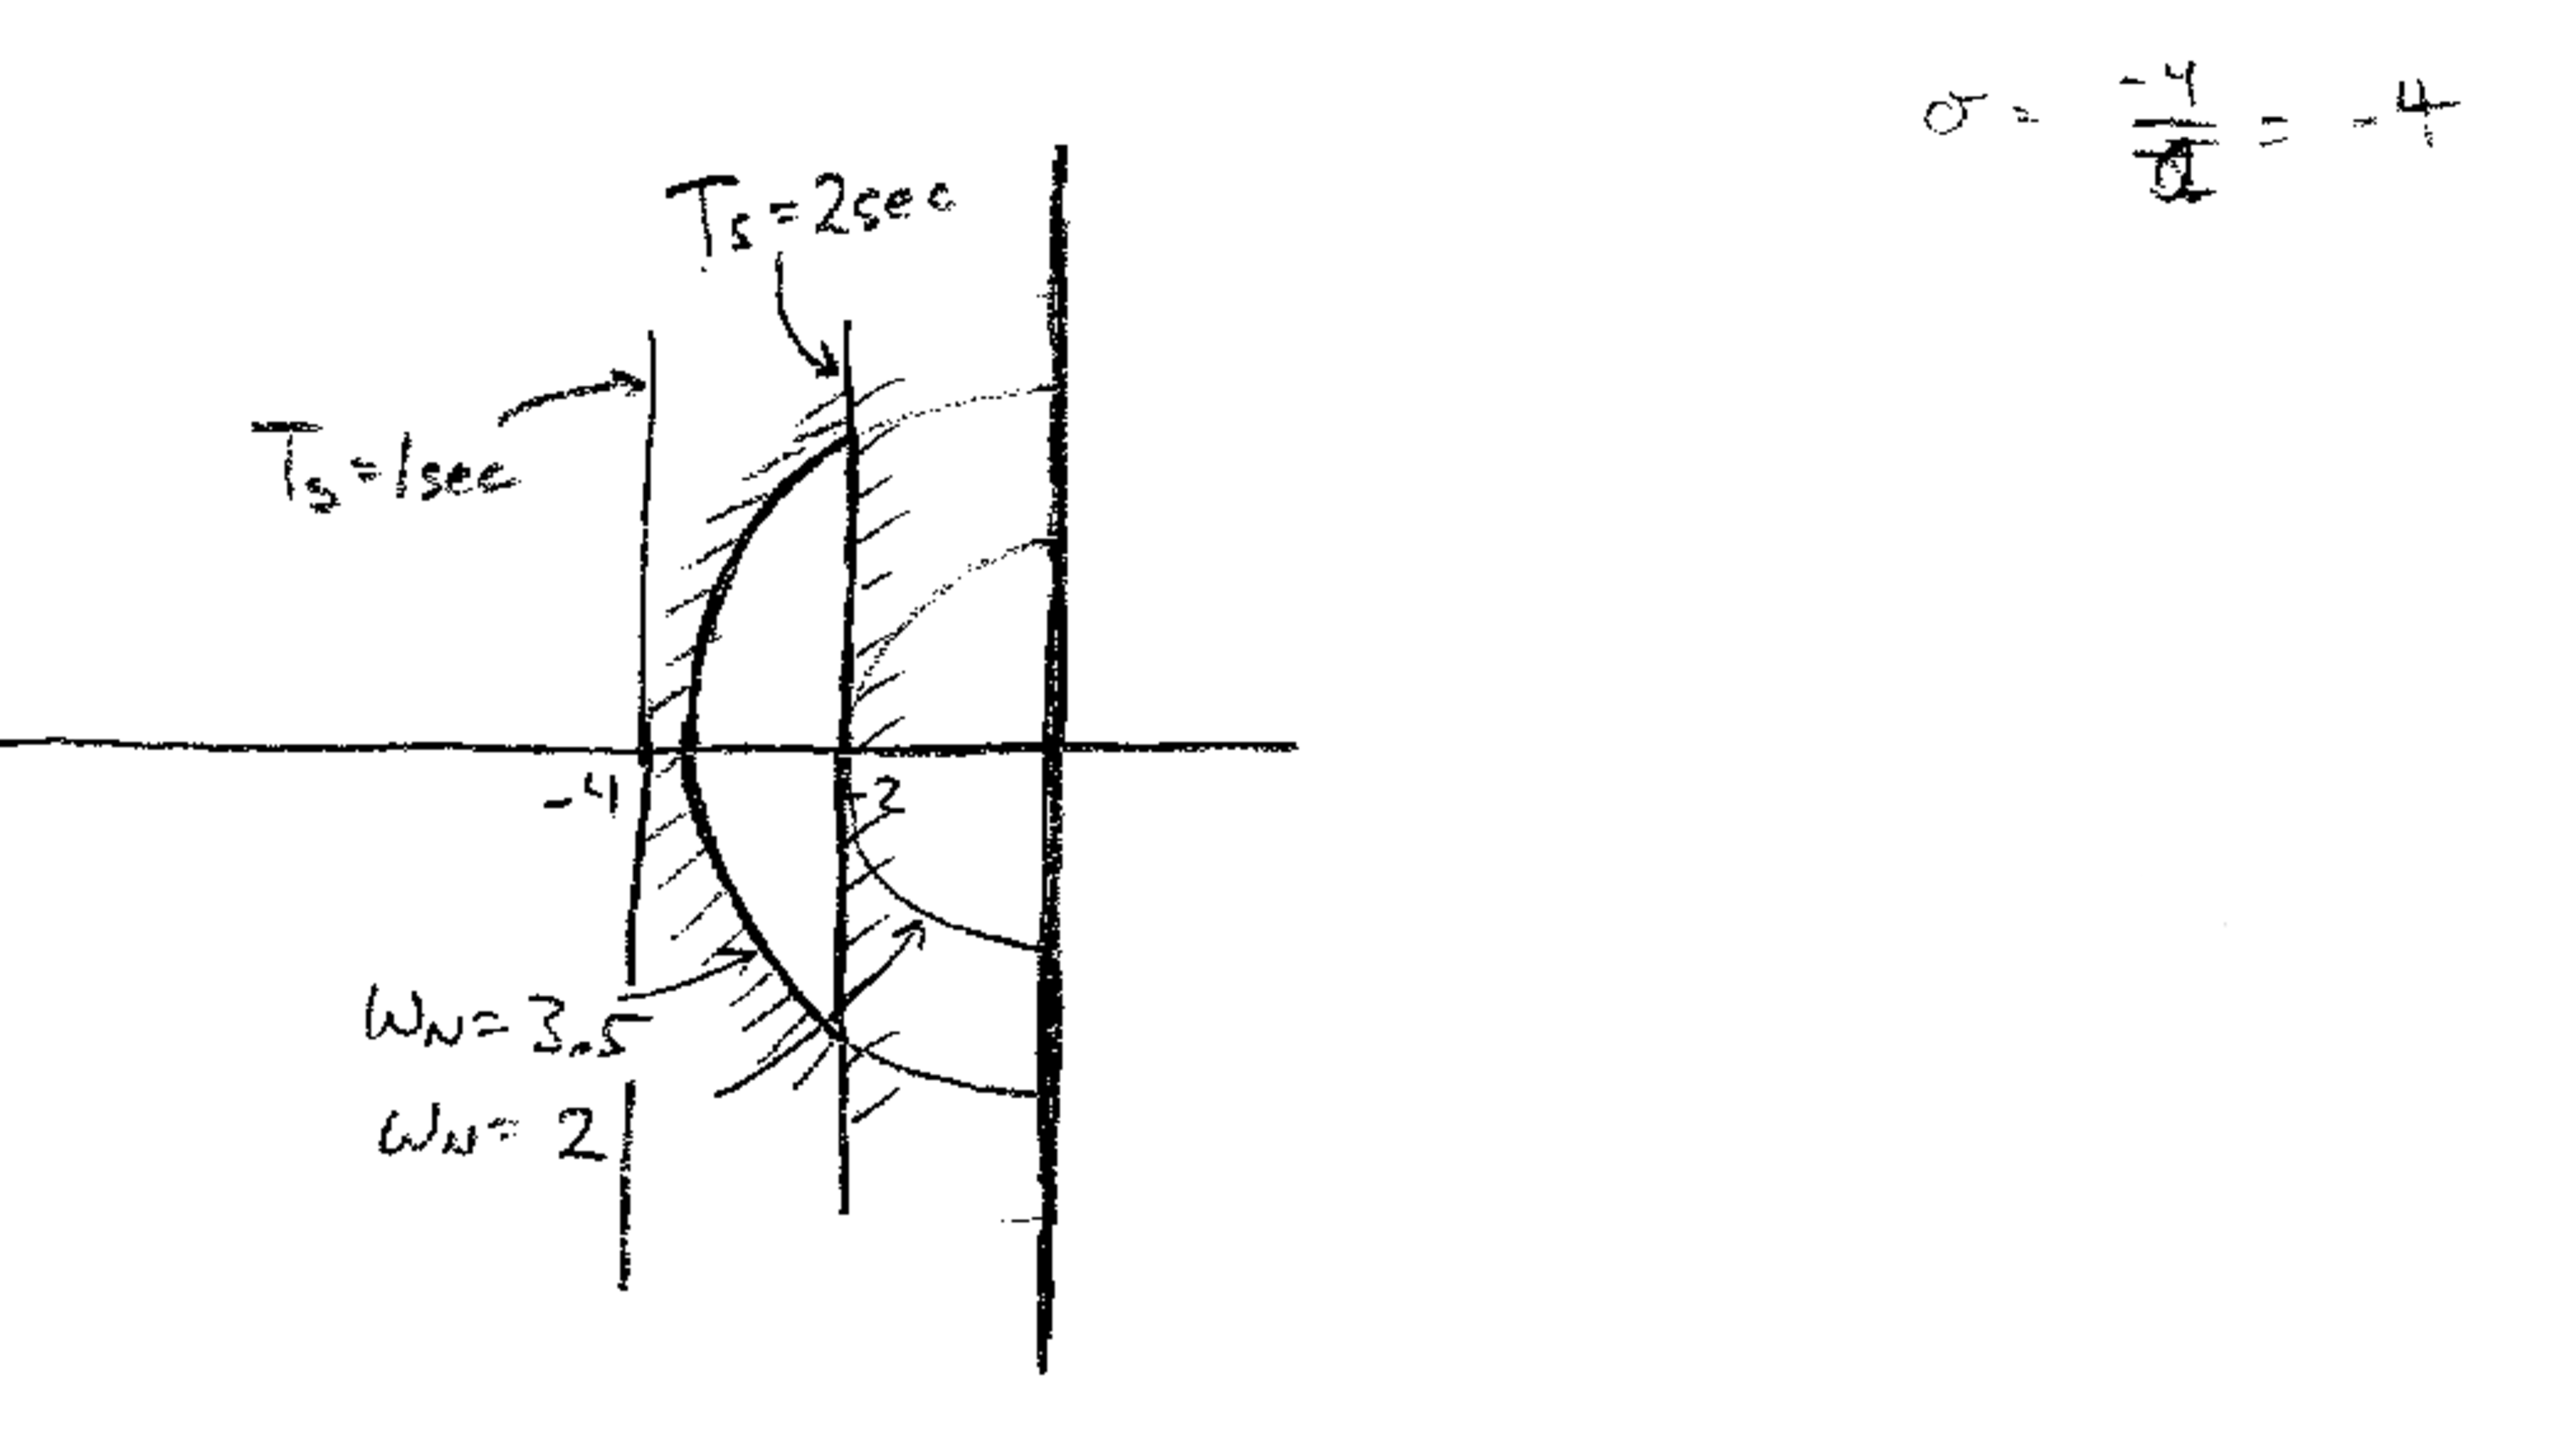
\includegraphics[width=12cm]{00549a.png}	%<n>





%%%%%%%%%%%%%%%%%%%%%%%%%%%%%%%%%%%%%%%%%%%%%%%%%%%%%%%%%%%%%%%%%%%%%%%%%%%%%%%%%%%%%%%%%%%%%%%%%%%%%%%%%%%%%%%%%%%%%%%%%%%%%%%%%%%%

	%<*>
%%%%** Section 7.5
\subsection{}  Identify the point or region of the s-plane corresponding to:

%%%%** Section 7.5.1 
\subsubsection{}    $T_S = 0.8$sec, \%OS = 5\%

%%%%** Section 7.5.2 
\subsubsection{}    $T_S \leq 10$sec, \%OS = 10\%

%%%%** Section 7.5.3 
\subsubsection{}    $T_S \leq 5$sec, \%OS $\leq$ 2\%


	%<*n>
\begin{solution}

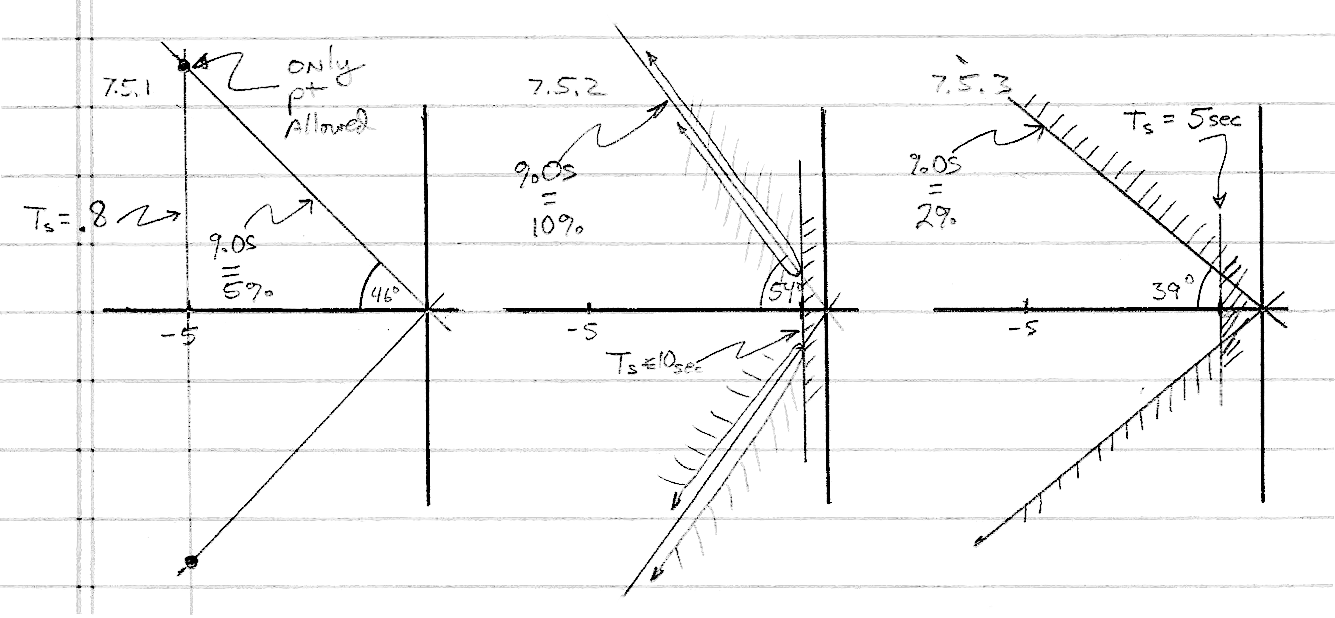
\includegraphics[width=6.5in]{01121.png}

\end{solution}
	%<*>




%%%%%%%%%%%%%%%%%%%%%%%%%%%%%%%%%%%%%%%%%%%%%%%%%%%%%%%%%%%%%%%%%%%%%%%%%%%%%%%%%%%%%%%%%%%%%%%%%%%%%%%%%%%%%%%%%%%%%%%%%%%%%%%%%%%%

	%<*>
%%%%** Section 7.6
\subsection{Manual PID Design}\label{manualdesign1}


Manually estimate PID controller parameters, $K_P, K_I, K_D$ for the following system (you may use the computer for Root Locus).

\[
P(s) = \frac  {100(s+0.1)}   {s^2+2\zeta\omega_ns + \omega_n^2}
\]
where
\[
\omega_n = 2.0, \qquad \zeta = 0.875
\]
to achieve the following specs:

\[
T_s = 0.075, \quad \%OS = 5\%
\]




	%<*n>
\begin{solution}
\[
P(s) = \frac{100(s+0.1)}{s^2+3.5s+4}
\]
S-plane specs:
\[
\sigma = \frac {-4} {0.075} = -53, \qquad 5\%OS \to 46^\circ
\]
Plotting the OL poles and zeros:

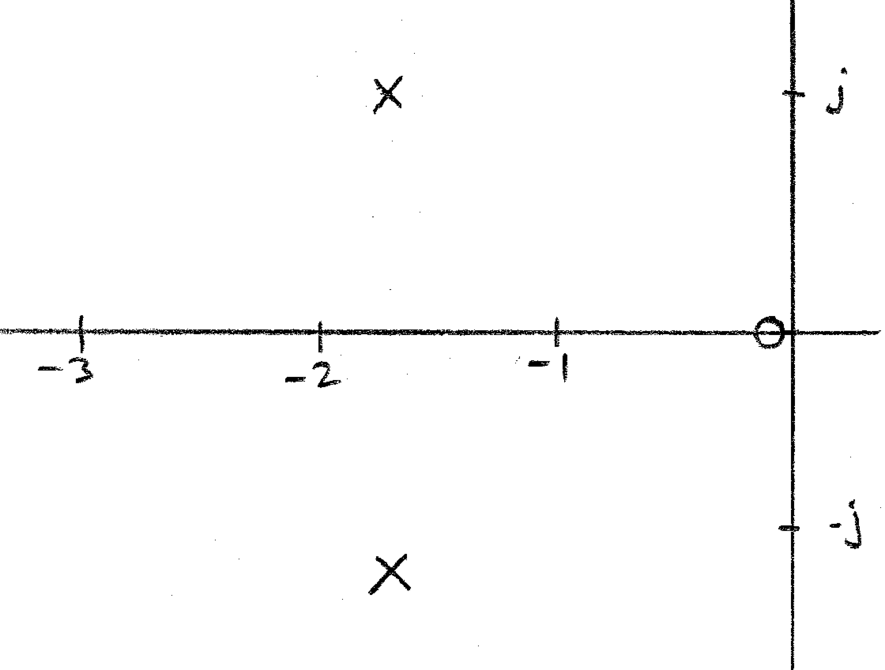
\includegraphics[width=75mm]{00956a.png}

We need to move WAY to the left to meet the $T_s$ spec!!    Let's synthesize a PID controller having zeros fairly far beyond -53.   First guestimate:
\[
z_1 = -70, \quad z_2  = -100, \quad pp = -250s
\]
Using one of the forms of the PID controller:
\[
C(s) = \frac  {K_D(s+z_1)(s+z_2)}   {s(s+250)}
\]
(pp is the ``regularization pole")

Computing root locus in Scilab and drawing on it with pencil:


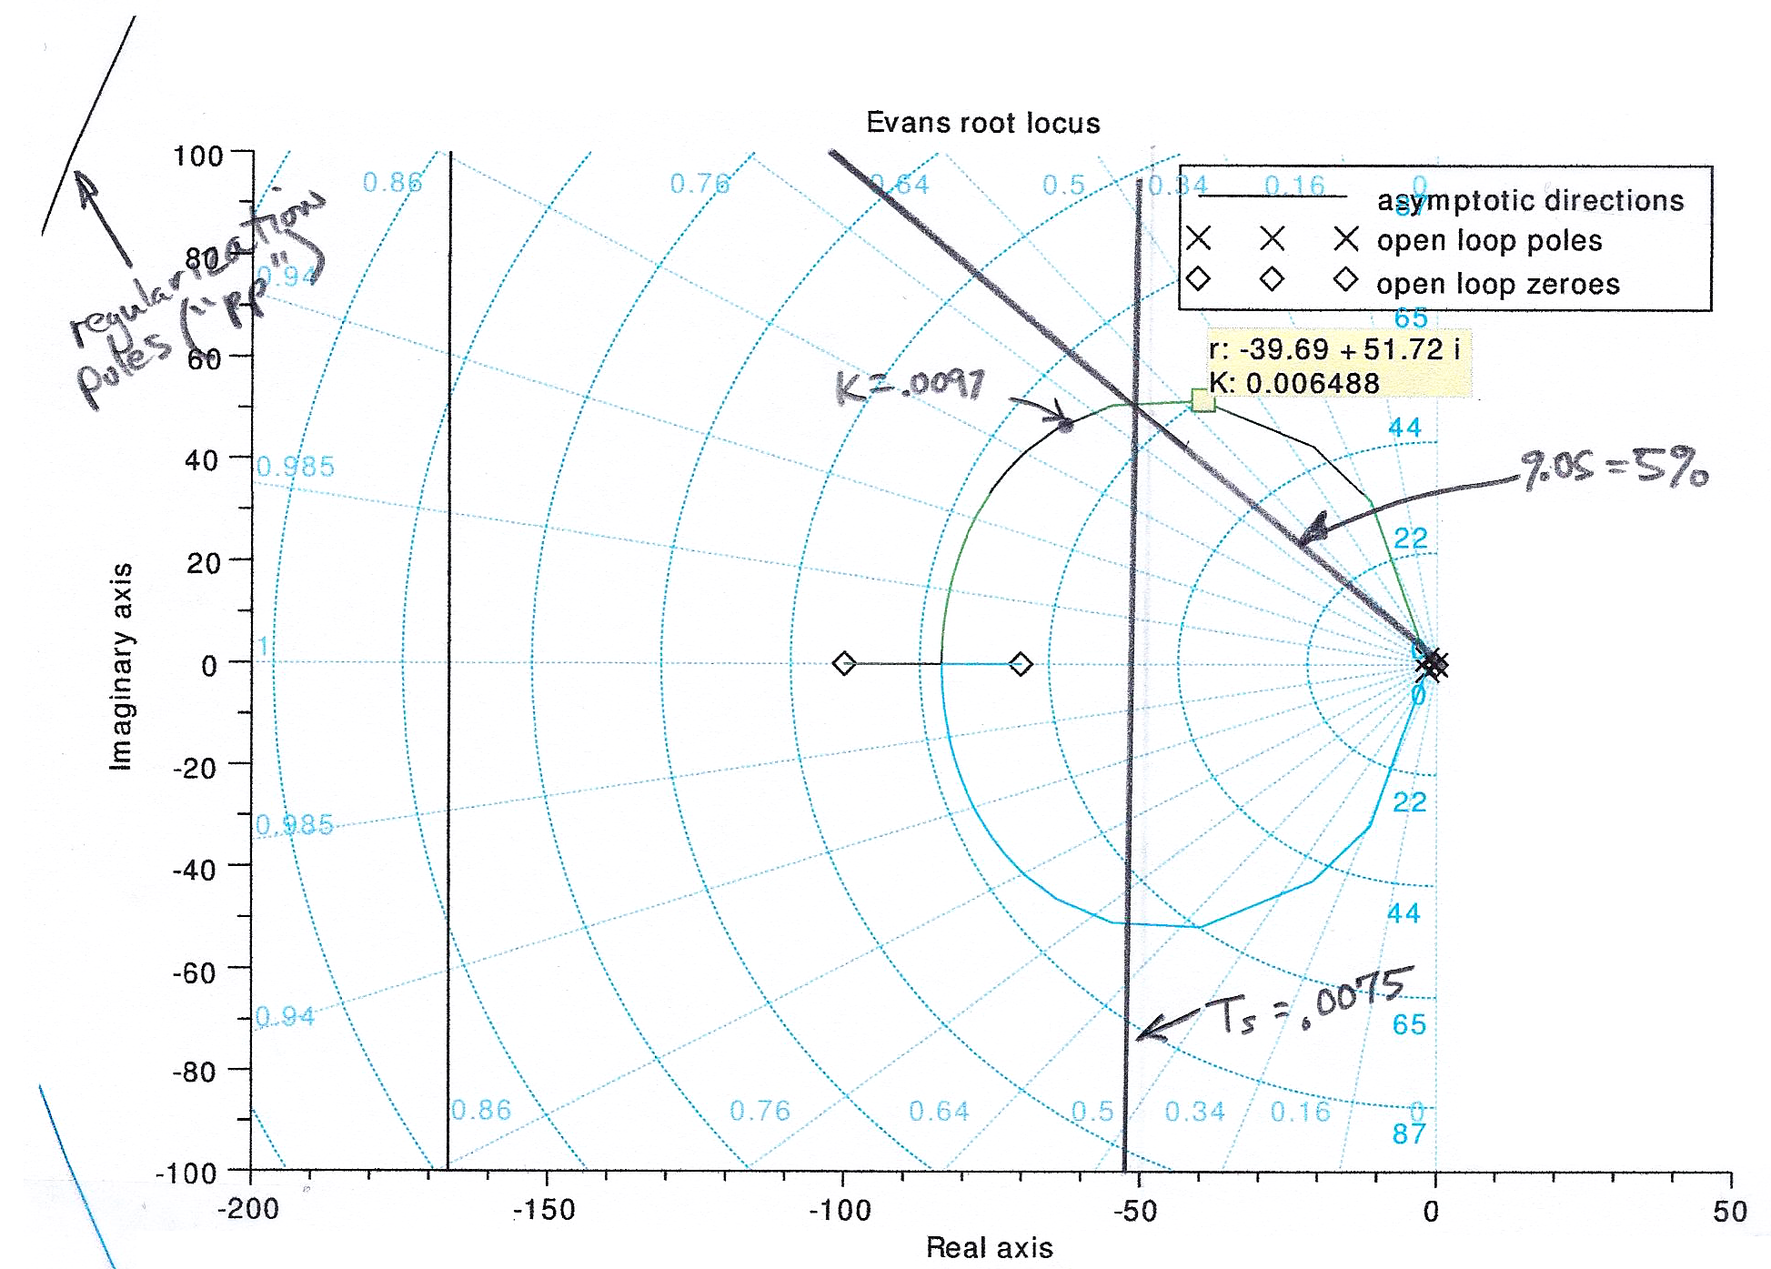
\includegraphics[width=150mm]{00957a.png}

Best point seems to be clicking just inside the specs giving $K= 0.0097$ (same as $K_D = 0.0097$).  Now we can complete the controller:
\[
C(s) = \frac{0.0097(s+70)(s_100)}{s} = \frac{0.0097(s^2+170s+7\times10^4)}{s}
\]
\[
C(s) = 0.0097s + 1.65 + 679/s
\]
From this
\[
K_P = 1.65,\quad K_I=679,\quad K_D=0.0097
\]
is a decent starting point for computer optimization.
\end{solution}
	%<*>




%%%%%%%%%%%%%%%%%%%%%%%%%%%%%%%%%%%%%%%%%%%%%%%%%%%%%%%%%%%%%%%%%%%%%%%%%%%%%%%%%%%%%%%%%%%%%%%%%%%%%%%%%%%%%%%%%%%%%%%%%%%%%%%%%%%%
	%<*>
%%%%** Section 7.7
\subsection{}\label{manualdesign2}

Manually estimate PID controller parameters, $K_P, K_I, K_D$ for
\[
P(s) = \frac  {26.7}{(s+1)(s+4)}
\]

to achieve:

\[
T_s = 0.75, \quad \%OS = 10\%
\]
(you may use the computer for Root Locus).

	%<*n>
\begin{solution}
Specs:
\[
0.75 = \frac{-4}{\sigma} \qquad \%OS=10\% \to 54^\circ
\]

Because these are equalities, there is only a point solution goal ($-5.333\pm8j$), not a region in the s-plane:

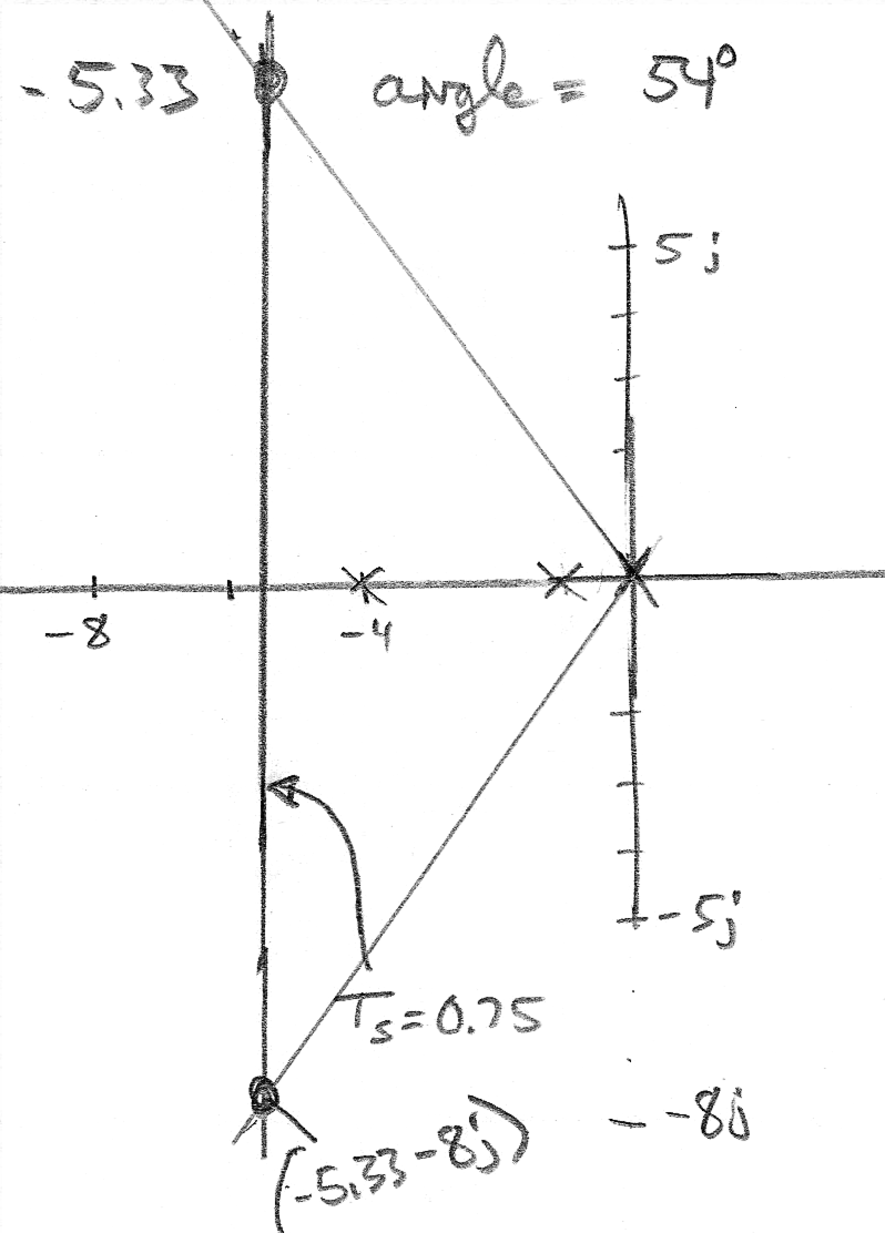
\includegraphics[width=75mm]{00958a.png}

Try \#1:
\[
z = -10\pm10j \quad (K_{max} = 100)
\]
\paragraph{Result:}  poles circle around the target but do not reach it.


Try \#2:
\[
z = -10\pm j
\]

\paragraph{Result:}  poles go way out to meet the regularization pole!.

Try \#3:
\[
z = -8\pm5j
\]

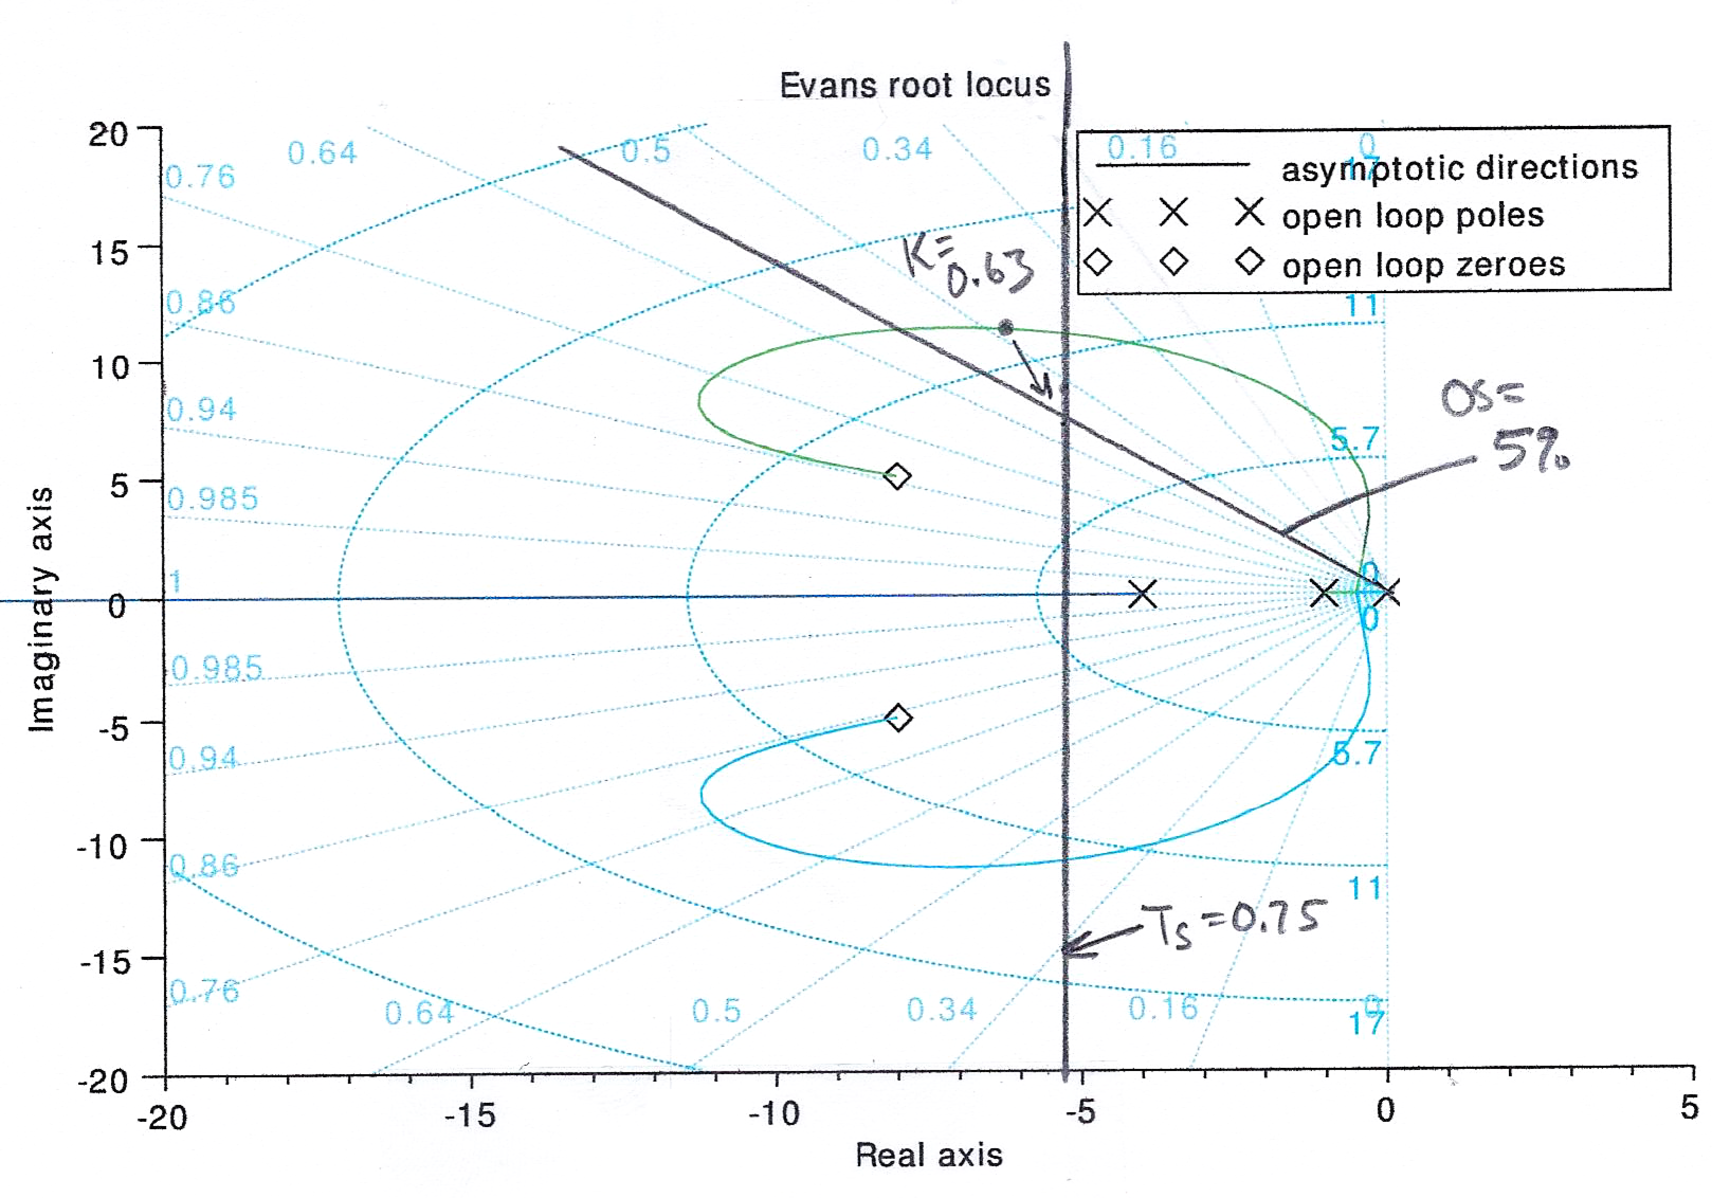
\includegraphics[width=145mm]{00959a.png}

\paragraph{Result:}  pretty close!

Clicking the closest point on the RL to the goal gives $K=0.63$.  Plugging in (as in previous problem):

\[
C(s) = \frac{0.63(s^2+16s+89)}{s}
\]

\[
K_P = 10.1,\quad K_I = 56.1, \quad K_D=0.63
\]





\end{solution}
	%<*>




%%%%%%%%%%%%%%%%%%%%%%%%%%%%%%%%%%%%%%%%%%%%%%%%%%%%%%%%%%%%%%%%%%%%%%%%%%%%%%%%%%%%%%%%%%%%%%%%%%%%%%%%%%%%%%%%%%%%%%%%%%%%%%%%%%%%
	%<*>
%%%%** Section 7.8
\subsection{Gain Margin and Phase Margin}
{\bf (if time)}  Consider a closed loop system where
\[
C(s) = \frac{K}{(s+10)} \qquad P(s) = \frac{500(s+1)}{(s+0.1)(s+25)(s+200)} \qquad H(s) = 1
\]


	%<*>
%%%%** Section 7.8.1 
\subsubsection{}  Plot the Bode Magnitude and Phase Diagrams of $CPH(s)$ by hand for $K=100$.

	%<*n>
{\tt SOLUTION: (see next sub-problem)} 


	%<*>
%%%%** Section 7.8.2 
\subsubsection{}   Using your Bode plot from the previous section, compute the Phase and Gain Margins.

	%<*n>
{\tt SOLUTION: }

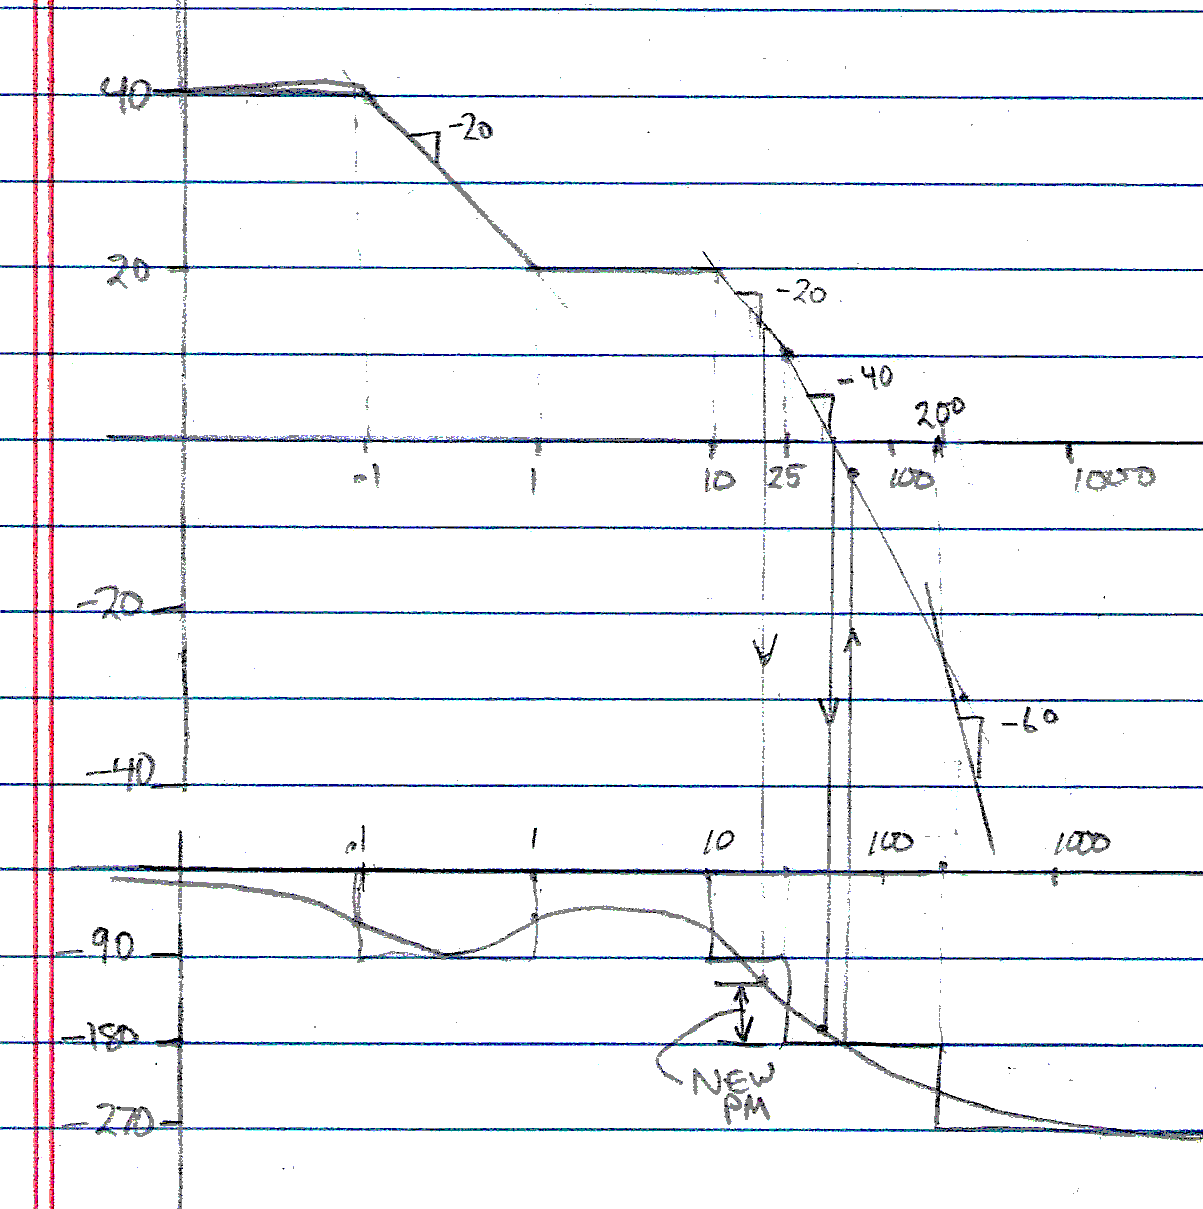
\includegraphics[width=5.5in]{bode_gm_pm}

Starting at the point where the loop gain, $CPH(s)$ has magnitude 1 (0$dB$), we go down to the phase curve and note an angle of about -$170^\circ$.  This is a Phase Margin of $10^\circ$.
Then, looking at the point where the Phase curve crosses -180$^\circ$, we go back up and note the gain is about $-3dB$. Thus the phase margin is $3dB$ because we need to $add$ $3dB$ to get up to zero.
	%<*>


	%<*>
%%%%** Section 7.8.3 
\subsubsection{}  Find a value of $K$ to get a Gain Margin of $15dB$.  What is the new Phase Margin?

	%<*n>
{\tt SOLUTION: }

To find a value of $K$ for the specified Gain Margin, note that the phase curve is unchanged for any real value of $K$.   Thus we can increase the GM to $15dB$ by just reducing $K$ by $12dB$ from $40dB$ to $28dB$.  $28dB$ is equivalent to a new $K=10^{1.4} = 25.1$.

Phase Margin:  Looking back at the magnitude curve, if we shift it down by $12dB$, we see it crosses 1 at a frequency just above 25.  At that frequency we go down to the Phase curve and get a new phase margin of about $75^\circ$.


	%<*>
%%%%** Section 7.8.4 
\subsubsection{}    Verify your answer with the Scilab ``Margins" command.


 {\tt SOLUTION:}	%<*n>

Using the following Scilab code:
\begin{verbatim}
//  EE447 ICP 7.2.4
//   Compute gain and phase margins.

clear all;
s = poly(0, 's');
K =100;
c = K / (s+10) ;
p = (500*(s+1)) / ((s+0.1)*(s+25)*(s+20)) ;
ctl   = syslin('c', c);
plant = syslin('c', p);
h     = syslin('c', s/s);
lg = ctl*plant*h;    //  CPH(s)

show_margins(lg);
gm = g_margin(lg);
pm = p_margin(lg);

printf("K = %6.1f\n",K);
printf("Phase Margin: %6.1f (deg)\n",pm);
printf("Gain  Margin: %6.1f (dB) \n",gm);
\end{verbatim}
We find that the system is actually unstable and our hand-computed margins are a bit off:
\begin{verbatim}

K =  100.0
Phase Margin:   -3.4 (deg)
Gain  Margin:   -1.0 (dB)
\end{verbatim}

When $K=25$ (as solved above), we get a better result but not as big a gain margin as required:
\begin{verbatim}

K =   25.0
Phase Margin:   55.2 (deg)
Gain  Margin:   11.1 (dB)
\end{verbatim}








	%<*>
%%%%%%%%%%%%%%%%%%%%%%%%%%%%%%%%%%%%%%%%%%%%%%%%%%%%%%%%%%%%%%%%%%%%%%%%%%%%%%%%%%%%%%%%%%%%%%%%%%%%%%%
\newpage
%%%%** Section 8 
\section{PID Controller Design with Scilab}

These ICP problems require the use of Scilab and the following scripts (provided by class website):
\begin{itemize}
\item {\tt setup.sce}  (rename, save, and customize this for each individual problem)
\item {\tt stepperf.sce} (routines which compute $T_s, \%OS$, etc.)
\item {\tt optigainX.sce} (script which searches the PID design space and finds best design).
\item {\tt quickplot.sce} (Optional, easily get step response of your plant with any $K_P,K_I,K_D$). 
\end{itemize}

To report your result, give the best output you get as it is output by the software.  Example:
\begin{verbatim}

[       Balanced] Kp:  7.632634919  Ki:  0.0015567  Kd:  0.008297948
Settling Time:  0.04  Overshoot:  7.1 percent  SSE:  0.029  Ctl Effort:  0.78
  Search boundary reached:  Kp min Ki max Kd min

\end{verbatim}
 
	%<*>
%%%%** Section 8.1
\subsection{}
 Enter the following systems into Scilab:

(don't forget to initialize $s$ first)

A) \[
\frac{10^4(s+4)}{(s+50)(s+800)}
\]

B) \[
\frac{3200}{(s^2+34s+3200)}
\]

Use the {\tt csim()} command to plot the step responses.

(This is just to verify that you have Scilab set up and you know how to properly enter system equations.)

	%<*n>
\begin{solution}
{\tt For solution please see Scilab script icp7.sce }  % closed-loop-system-a = feedback(system-a, H=1) }

\end{solution}
	%<*>




	%<*>
%%%%** Section 8.2
\subsection{}
Using the provided Scilab tools, find PID controller parameters, $K_P, K_I, K_D$ for the following system

\[
P(s) = \frac  {100(s+0.1)}   {s^2+2\zeta\omega_ns + \omega_n^2}
\]
where
\[
\omega_n = 2.0, \qquad \zeta = 0.875
\]
to achieve the following specs:

\[
T_s = 0.075, \quad \%OS = 5\%, \quad Cu = 1.0
\]

Initialize your search range using the results of ICP \ref{manualdesign1}.

	%<*n>
\begin{solution}

\subsection*{Best optimization search results:}
\begin{verbatim}

[       Balanced] Kp:  4.849073128  Ki: 34.499334510  Kd:  0.002299956
Settling Time:  0.01  Overshoot:  2.0 percent  SSE:  0.006  Ctl Effort:  2.82

Search Time:  1.8 minutes.  N = 3375  (  1928.6 sims/min)

\end{verbatim}

\end{solution}




	%<*>
%%%%** Section 8.3
\subsection{}


Using the provided Scilab tools, find a PID controller for
\[
P(s) = \frac  {26.7}{(s+1)(s+4)}
\]

For

\[
T_s = 0.75, \quad \%OS = 10\%,\quad SSE \leq 3\%, \quad Cu = 50.0
\]

Initialize your search range using the results of ICP \ref{manualdesign2}.

	%<*n>
\begin{solution}

\subsection*{Best optimization search results:}
\begin{verbatim}

[       Balanced] Kp:  1.263  Ki:  0.938  Kd:  0.099
Settling Time:  0.85  Overshoot:  9.1 percent  SSE:  0.001  Ctl Effort: 79.20
  Search boundary reached:  Kd max
\end{verbatim}

\end{solution}




	%<*>
%%%%** Section 8.4
\subsection{}
Wind turbine speed via blade pitch control (Dorf, Example 9.10, p675)
\[
P(s) = \frac {7000\omega_n^2} {(\tau s + 1)(s^2+2\zeta\omega_ns + \omega_n^2)}
\]
Where
\[
\tau = 5.0, \quad \omega_n = 20, \quad \zeta = 0.005
\]
to achieve:
\[
T_s =  20 sec, \quad \%OS = 20.0\%, \quad Cu = 0.001
\]


{\bf   Hint: start with Kp = 0.0001 and go even smaller with Kp, Kd. }

	%<*n>
\begin{solution}
Try:

Kp = 0.000126, Ki = 0.0000949, Kd = 0.00000158

(Dorf: Kp = 3.1E-05, KI = 1.2E-4, Kd = 6.2E-6)

\begin{verbatim}

[       Balanced] Kp:  0.000098031  Ki:  0.000123329  Kd:  0.000001961
Settling Time: 19.20  Overshoot: 26.4 percent  SSE:  0.001  Ctl Effort:  0.00
  Search boundary reached:  Kp max Kd min

\end{verbatim}

\end{solution}




	%<*>
%%%%** Section 8.5
\subsection{}
Flexible Robot Arm: (Dorf Design Problem 9.2 p737)
\[
P(s) =   \frac {1}{s^2 + 9s + 12}
\]

For

\[
T_s =  2.0 sec, \quad \%OS = 20.0\%, \quad Cu = 40
\]

	%<*n>
\begin{solution}

Try:

Kp = 51.2, Ki = 114.7, KD = 0.079

Another (similar) result:

\begin{verbatim}

[       Balanced] Kp: 23.343  Ki: 68.884  Kd:  0.238
Settling Time:  2.00  Overshoot: 20.4 percent  SSE:  0.000  Ctl Effort: 28.54
  Search boundary reached:  Kd min
\end{verbatim}
\end{solution}




	%<*>
%%%%** Section 8.6
\subsection{}
Radar Tracking System: (Phillips and Parr, p275))
\[
P(s) = \frac{1}{s(s+2)}
\]
To get

\[
T_s =  8 sec, \quad \%OS = 5\%, \quad Cu = 10
\]

	%<*n>
\begin{solution}

[       Balanced] Kp:  4.179  Ki:  0.411  Kd:  0.103
Settling Time:  8.40  Overshoot: 23.7 percent  SSE:  0.001  Ctl Effort:  3.60

 \begin{verbatim}
\end{verbatim}
\end{solution}








	%<*>
%%%%** Section 8.7
\subsection{}
Voltage control system (Phillips and Parr, p276)

\[
P(s) =  \frac {1}{(s+1)(s+2)}
\]
To get

\[
T_s =  1.0 sec, \quad \%OS = 5\%, \quad Cu = 150
\]
	%<*n>
\begin{solution}

\begin{verbatim}
[       Balanced] Kp: 12.597  Ki:  6.870  Kd:  2.799
Settling Time:  1.15  Overshoot:  4.3 percent  SSE:  0.003  Ctl Effort: 55.99
\end{verbatim}

\end{solution}



	%<*>


%%%%%%%%%%%%%%%%%%%%%%%%%%%%%%%%%%%%%%%%%%%%%%%%%%%%%%%%%%%%%%%%%%%%%%%%%%%%%%%%%%%%%%%%%%%%%%%%%%%%%%
\newpage
%%%%** Section 9 
\section{EE447 ICP 9: Discrete time implementation of controllers.}


%%%%** Section 9.1
\subsection{Sampling Theorem }


An analog signal has bandwidth 25 Hz.   What is the minimum necessary sampling frequency necessary to reconstruct the signal without distortion?


	%<*n>
\begin{solution}
\[
f_N = 2b = 50 Hz
\]
\end{solution}
	%<*>

%%%%** Section 9.2
\subsection{Tustin's Method}


A controller has the continuous time transfer function:
\[
C_1(s) = \frac{1000}{(s+7.5)}
\]
Apply Tustin's method to convert it into a discrete time controller with sampling time $T=0.01$.


	%<*n>
\begin{solution}
\[
C_1(z) = \frac{1000}{\frac{2(z-1)}{T(z+1)} + 7.5}
\]
\[
= \frac{10(z+1)}{2z-2+0.075z + 0.075} = 4.82\frac{(z+1)}{(z-0.9277)}
\]
\end{solution}
	%<*>



%%%%** Section 9.3
\subsection{Tustin's Method}


A controller has the continuous time transfer function:
\[
C_2(s) = \frac{50(s+2)}{(s+0.1)(s+50)}
\]
Apply Tustin's method to convert it into a discrete time controller with sampling time $T=0.001$.

	%<*n>
\begin{solution}
Applying Tustin's method:

\[
C_2(s) = \frac{50(s+2)}{s^2+50.1s+5}
\]
Applying Tustin's method, simplifying this through several steps and using $T=0.001$, gives:
\[
C_2(z) = 0.0244\frac  {z^2+0.001998z - 0.998890}   {z^2-1.95112z+0.951125}
\]
\end{solution}
	%<*>



%%%%** Section 9.4
\subsection{Conversion to digital filter}


Convert the following discrete time controller to a digital filter:

\[
C_3(z) = 30\frac{(z+1)}{(z+0.997)}
\]

Express your digital filter in a form which can be directly coded into software.


	%<*n>
\begin{solution}
\[
C_3(z) = \frac{F(z)}{E(z)}
\]
\[
30(zE(z) + E(z)) = (z+0.997)F(z)
\]
multiply through by $z^{-1}$:
\[
30E(z) + 30z^{-1}e(z) = F(z)+ 0.997z^{-1}F(z)
\]
Inverse Transform:
\[
30e(n) + 30e(n-1)  = f(n) + 0.997f(n-1)
\]
rearranging:
\[
f(n) = 30e(n) + 30e(n-1) - 0.997f(n-1)
\]
\end{solution}
	%<*>


%%%%** Section 9.5
\subsection{Conversion to digital filter}


Convert the following discrete time controller to a digital filter:

\[
C_4(z) = 10^3\frac{(z+1)}{(z+0.76)(z+0.997)}
\]



	%<*n>
\begin{solution}
\[
C_4(z) = 10^3\frac{(z+1)}{z^2+1.757z+0.758} = \frac{U(z)}{E(z)}
\]
\[
z^2U(z)+1.757zU(z)+0.758U(z) = 10^3(zE(z)+E(z))
\]
\[
U(z)+1.757z^{-1}U(z)+0.758z^{-2}U(z) = 10^3(z^{-1}E(z)+z^{-2}E(z))
\]

\[
u(n) = 10^3(e(n-1)+e(n-2))-1.757u(n-1)-0.758u(n-2)
\]
\end{solution}

	%<*>
\end{document}

